\documentclass{tufte-book}
% chapter format

\usepackage{amsthm,thmtools,xcolor}
\setcounter{tocdepth}{3}
\setcounter{secnumdepth}{3}
%% paleta 1
%\definecolor{mycolor1}{RGB}{8,32,50}
%\definecolor{mycolor2}{RGB}{44,57,75}
%\definecolor{mycolor3}{RGB}{51,71,86}
%\definecolor{mycolor4}{RGB}{255,76,41}

%%% paleta 2
%\definecolor{mycolor1}{RGB}{17,29,94}
%\definecolor{mycolor2}{RGB}{199,0,57}
%\definecolor{mycolor3}{RGB}{243,113,33}
%\definecolor{mycolor4}{RGB}{192,226,24}

%% paleta 3
%\definecolor{mycolor1}{RGB}{75,93,103}
%\definecolor{mycolor2}{RGB}{50,47,61}
%\definecolor{mycolor3}{RGB}{89,64,92}
%%\definecolor{mycolor4}{RGB}{135,85,111}
%
%% paleta 4
%\definecolor{mycolor1}{RGB}{26,26,46}
%\definecolor{mycolor2}{RGB}{22,33,62}
%\definecolor{mycolor3}{RGB}{15,52,96}
%\definecolor{mycolor4}{RGB}{233,69,96}

% paleta 6
\definecolor{mycolor1}{RGB}{251, 54, 64}
\definecolor{mycolor2}{RGB}{96, 95, 94}
\definecolor{mycolor3}{RGB}{29, 52, 97}
\definecolor{mycolor4}{RGB}{31, 72, 126}
\definecolor{mycolor5}{RGB}{36, 123, 160}

\colorlet{ColorVariable1}{mycolor1}
\colorlet{ColorVariable2}{mycolor2}
\colorlet{ColorVariable3}{mycolor3}
\colorlet{ColorVariable4}{mycolor4}
\colorlet{ColorVariable5}{mycolor5}

\hypersetup{
	pdftitle={Precálculo},
	pdfauthor={Juliho Castillo Colmenares},
	colorlinks=true,	
	linkcolor=ColorVariable5,
	anchorcolor=ColorVariable5,
	runcolor=ColorVariable5,		
	filecolor=ColorVariable5,
	citecolor = ColorVariable5,      
	urlcolor=ColorVariable5,
	frenchlinks=true
}

\titleformat{\chapter}%
{\huge\rmfamily\itshape\color{ColorVariable4}}% format applied to label+text
{\llap{\colorbox{ColorVariable4}{\parbox{1.5cm}{\hfill\itshape\huge\color{white}\thechapter}}}}% label
{2pt}% horizontal separation between label and title body
{}% before the title body
[]% after the title body

% section format
\titleformat{\section}%
{\normalfont\Large\itshape\color{ColorVariable4}}% format applied to label+text
{\llap{\colorbox{ColorVariable4}{\parbox{1.5cm}{\hfill\color{white}\thesection}}}}% label
{1em}% horizontal separation between label and title body
{}% before the title body
[]% after the title body

% subsection format
\titleformat{\subsection}%
{\normalfont\large\itshape\color{ColorVariable4}}% format applied to label+text
{\llap{\colorbox{ColorVariable4}{\parbox{1.5cm}{\hfill\color{white}\thesubsection}}}}% label
{1em}% horizontal separation between label and title body
{}% before the title body
[]% after the title body


%\newenvironment{problema}{
	%	\medskip
	%	%\begin{framed}
	%	\bgroup\color{ColorVariable1}
	%	{\textbf{Problema.}}
	%}{
	%	\egroup
	%	%\end{framed}
	%	\medskip
	%}

\declaretheoremstyle[
headfont=\color{ColorVariable1}\normalfont\bfseries,
bodyfont=\color{ColorVariable2}\normalfont\itshape,
]{colored}

\declaretheoremstyle[
headfont=\color{ColorVariable3}\normalfont\bfseries,
bodyfont=\color{ColorVariable3}\normalfont\itshape,
]{colored-2}

\declaretheorem[
style=colored,
name=Problema,
numberwithin=section, 
%shaded={rulecolor=Lavender,
	%	rulewidth=2pt, 
	%	bgcolor={rgb}{1,1,1}}
]{problema}

\declaretheorem[
style=colored,
name=Problema Resuelto,
numberwithin=section, 
%shaded={rulecolor=Lavender,
	%	rulewidth=2pt, 
	%	bgcolor={rgb}{1,1,1}}
]{resuelto}

\declaretheorem[
style=colored,
name=Solución,
numbered = no
]{solucion}

\declaretheorem[
style=colored,
name= Ejemplo,
numberwithin=section
]{ejemplo}

\declaretheorem[
style=colored-2,
name= Definición,
numbered = no
]{definicion}

\newenvironment{algoritmo}[1]{
	\medskip
	%\begin{framed}
	\bgroup
	\color{ColorVariable3}
	{\textbf{Algoritmo. (#1)}}
	\ttfamily
}{
	\egroup
	%\end{framed}
	\medskip
}

%\newtheorem{teorema}{Teorema}%[chapter]

\declaretheorem[
style=colored,
name=Teorema,
]{teorema}

%\newtheorem{proposicion}{Proposición}%[chapter]

\declaretheorem[
style=colored,
name=Proposición,
]{proposicion}

%\newtheorem{observacion}{Observación}%[chapter]

\declaretheorem[
style=colored-2,
name=Observación,
numbered = no
]{observacion}

\newtheorem{axioma}{Axioma}%[chapter]
\newtheorem{sugerencia}{Sugerencia}%[chapter]
\newtheorem{corolario}{Corolario}%[chapter]
\usepackage{fontenc}
\usepackage{graphicx}
\usepackage[utf8]{inputenc}
\usepackage[spanish,mexico]{babel}
\usepackage{fontenc}
\usepackage{amsmath}
\usepackage{amssymb}
\usepackage{graphicx}
\usepackage{mathrsfs}
\usepackage{yfonts}
\usepackage{enumerate}
\usepackage{mathtools}
\usepackage{textcomp}
\usepackage{lmodern}
\usepackage{fancyvrb}
\usepackage{multicol}
\usepackage{wrapfig}
\usepackage{floatflt}
\usepackage{filecontents}
\usepackage{hyperref}
%\usepackage{bibentry}
\usepackage{graphicx} % Allows including images
\usepackage{booktabs} % Allows the use of \toprule,
\usepackage{mdframed}
\usepackage[dvipsnames]{xcolor}
\usepackage{tikz}
\usepackage{amsthm}
\usepackage{hyperref}
\usepackage{listings}
\usepackage{units}
\usepackage{color}
%\newenvironment{solucion}{\begin{proof}[Solución]}\begin{color}{red}\end{color}{\end{proof}}

\usetikzlibrary{matrix,arrows,decorations.pathmorphing}
 
\hypersetup{
	pdftitle={Estadística Matemática},
	pdfauthor={Juliho Castillo Colmenares},
	colorlinks=true	
%	linkcolor=BrickRed,
%	filecolor=BrickRed,
%	citecolor = BrickRed,      
%	urlcolor=BrickRed,
	%frenchlinks=true
}


%%% MANDATORY!!!

\newcommand{\R}{\mathbb{R}}
\newcommand{\N}{\mathbb{N}}
\newcommand{\Q}{\mathbb{Q}}
\newcommand{\C}{\mathbb{C}}
\newcommand{\Z}{\mathbb{Z}}

\newcommand{\set}[1]{\left\{ #1 \right\}}
\newcommand{\evat}[2]{\left. #1 \right|_{#2}}
\newcommand{\sett}[2]{\left\{ \left.#1 \right| #2 \right\} }

\newcommand{\inp}[1]{\langle #1 \rangle}
\newcommand{\norm}[1]{\left\| #1 \right\|}
\newcommand{\abs}[1]{\left|#1\right|}
\newcommand{\imply}{\rightarrow}

%precalculo

\newcommand{\mcd}{mcd}
\newcommand{\mcm}{mcm}

% Calculo
\newcommand{\del}{\delta}
\renewcommand{\a}{\alpha}
\newcommand{\Del}{\Delta}
\newcommand{\sech}{sech}
\newcommand{\csch}{csch}
\newcommand{\ep}{\epsilon}
\newcommand{\p}{\partial}

%ecuaciones diferenciales
\newcommand{\lap}[1]{\mathcal{L}\set{#1}}
\newcommand{\lapin}[1]{\mathcal{L}^{-1}\set{#1}}
\newcommand{\lam}{\lambda}

%álgebra lineal

\renewcommand{\a}{\alpha}
\renewcommand{\b}{\beta}

\newcommand{\gen}[1]{\operatorname{gen}\left( #1 \right)}

\newcommand{\av}{\arrowvert}

\newcommand{\id}{\operatorname{Id}}

\newcommand{\im}{\mathfrak{I}}

\renewcommand{\Im}{\operatorname{Im}}

\newcommand{\nul}[1]{\operatorname{nul}\left( #1 \right)}
\newcommand{\ran}[1]{\operatorname{ran}\left( #1 \right)}

\newcommand{\ssi}{\Leftrightarrow}
\newcommand{\basis}[1]{\left( #1 \right)}
\renewcommand{\th}{\theta}
\renewcommand{\arg}[1]{\varphi(#1)}
\newcommand{\bm}[1]{\begin{bmatrix}#1\end{bmatrix}}

% probabilidad
\newcommand{\corr}{\rho}
\newcommand{\f}{\phi}
\newcommand{\vphi}{\varphi}
\newcommand{\vf}{\varphi}
\newcommand{\flow}[2]{\varphi^{#1}\left( #2 \right)}
\renewcommand{\d}[1]{\dot{#1}}
\renewcommand{\r}{\rho}
\newcommand{\A}{\mathcal{A}}
\newcommand{\gam}{\gamma}
\renewcommand{\a}{\alpha}
\renewcommand{\b}{\beta}
\newcommand{\om}{\omega}
\newcommand{\iso}{\simeq}
\newcommand{\tensor}{\otimes}
\newcommand{\inc}{\hookrightarrow}
\renewcommand{\L}{\mathcal{L}}
\renewcommand{\H}{\mathcal{H}}
\newcommand{\D}{\mathcal{D}}
\newcommand{\converge}[1]{\xrightarrow{#1}}
\newcommand{\cott}[1]{T^{*}\T^{#1}}
%\newcommand{\G}{\mathcal{G}}
\newcommand{\hu}{\textbf{h}}
\newcommand{\deck}[1]{\operatorname{Dake}\left( #1 \right)}
\newcommand{\til}[1]{\tilde{#1}}
\newcommand{\Gam}{\Gamma}
\newcommand{\grad}{\nabla}
\newcommand{\var}{\Delta}
\newcommand{\avch}[2]{\frac{\Delta #1}{\Delta #2}}
\newcommand{\Avch}[2]{\dfrac{\Delta #1}{\Delta #2}}
\newcommand{\Err}{\operatorname{Err}}
\newcommand{\wed}{\wedge}
\newcommand{\biconditional}{\longleftrightarrow}
\newcommand{\yields}{\vdash}
\newcommand{\onlyif}{\Rightarrow}
\newcommand{\uset}{\mathbb{U}}
\newcommand{\minus}{\backslash}
\newcommand{\symdif}{\oplus}
\newcommand{\rel}[1]{{ {\color{blue}\textbf{#1}} }}
\newcommand{\dominio}[1]{\operatorname{Dominio}\left( #1 \right)}
\newcommand{\imagen}[1]{\operatorname{Imagen}\left( #1 \right)}
\newcommand{\nrel}[1]{{ {\color{red}\not}{\color{orange}\textbf{#1}} }}
\newcommand{\comp}[2]{#1 \circ #2}

\renewcommand{\d}[1]{\dot{#1}}
\renewcommand{\r}{\rho}
\renewcommand{\a}{\alpha}
\renewcommand{\b}{\beta}
\renewcommand{\L}{\mathcal{L}}
\renewcommand{\H}{\mathcal{H}}

\newcommand{\Var}{\operatorname{Var}}
\newcommand{\s}{\sigma}
\newcommand{\comb}[2]{\begin{pmatrix} #1 \\ #2\end{pmatrix}}
\newcommand{\cov}{\operatorname{Cov}}


\title{Precálculo}
\author{github.com/julihocc}

\begin{document}
	\maketitle
\begin{tabular}{|p{.9\textwidth}|}
	\hline
Precálculo © 2020 by Juliho David Castillo Colmenares is licensed under Attribution 4.0 International
	\begin{center}
		
\includegraphics[scale=1]{./licencia/by.png}
	\end{center}\\
	\hline
\end{tabular}
\tableofcontents

\chapter{Teoría de conjuntos}
\section{Lógica matemática}


    Muchos algoritmos y demostraciones usan expresiones lógicas tales como
    \texttt{si p entonces q}. Entonces es necesario conocer los casos en los cuales esas expresiones son \texttt{ciertas} o \texttt{falsas}. Discutiremos esto en esta unidad. 

    Tambi\'en investigamos el valor de verdad de enunciados cuantificados, que son aquellos que usan los cuantificadores lógicos \texttt{para todo...} y \texttt{existe...}
    \marginnote{    	En este curso, usaremos el \emph{sistema algebráico de computo} \texttt{SageMath}, el cuál está escrito con base en el lenguaje de programación \texttt{Python} e incorpora diversos paquetes de \texttt{OpenSource}.  
    	Puede acceder a este sistema, a trav\'es de \href{https://cloud.sagemath.com/}{https://cloud.sagemath.com/} }


\subsection{Proposiciones y Declaraciones Compuestas}

    Una proposición es un enunciado declarativo que puede ser cierto o falso, pero no ambos. 

    \begin{problema}
        ?`Cuál de los siguientes enunciados es una proposición?
        \begin{multicols}{2}
            \begin{enumerate}
                \item El hielo flota en el agua.
                \item China está en Europa.
                \item $2+2=4$
                \item $2+2=5$
                \item ?`A donde vas?
                \item Haz tu tarea.
            \end{enumerate}
        \end{multicols}
    \end{problema}
    


\subsection{Proposiciones compuestas}


    Muchas proposiciones están \texttt{compuestas} de proposiciones más simples, llamadas \emph{subproposiciones}, por medio de \emph{conectores lógicos.}  Una proposición se dice que es \emph{primitiva} si no puede descomponerse en proposiciones más simples.



    Por ejemplo, las siguientes proposiciones son compuestas
    \begin{itemize}
        \item ``Las rosas son rojas y las violetas son azules''
        \item ``Juan es inteligente y estudia hasta muy noche''
    \end{itemize}
    



    La propiedad fundamental de una proposición compuesta es que su valor de verdad está completamente determinado por los valores de verdad de sus subproposiciones y la manera en la cual están conectadas para formar la proposición compuesta. 


\subsection{Operaciones Lógicas Básicas}


    En esta sección discutiremos las tres operaciones lógicas básicas: conjunción , disyunción  y la negación.


\subsection{Conjunción}


    Cualesquiera dos proposiciones $p,q$ pueden ser combinadas por la palabra ``y'' para formar una proposición compuesta llamada \emph{conjunción} que se escribe $p\wed q.$



    \begin{definicion}
        Si tanto $p$ como $q$ son ciertas, entonces $p \wed q$ es cierta; en otro caso $p\wed q$ es falsa.
        \sidenote{
        	\begin{tdv}[Conjunción]\hfill
        		\label{tdv:and}
        		\begin{center}
        			\begin{tabular}{|l|l|l|}\hline
        				$p$ & $q$ & $p \wed q$\\\hline
        				1 & 1 & 1\\\hline
        				1 & 0 & 0\\\hline
        				0 & 1 & 0\\\hline
        				0 & 0 & 0\\\hline
        			\end{tabular}
        		\end{center}        
        	\end{tdv}
        }  
    \end{definicion}	

    \begin{observacion}
        Para entender mejor como se conectan los valores de verdad, generalmente se utilizan \emph{tablas de verdad.}  
        
        Por brevedad $1$ representará el valor \texttt{cierto}, mientras que $0$ representará \texttt{falso}
    \end{observacion}
    
    	\marginnote{
    	Construimos la tabla de verdad de la conjunción en el siguiente script \href{https://cloud.sagemath.com/projects/12787063-cafe-4f3b-a2e0-905f8b83cf3b/files/MD01_TRDV01_AND.sagews}{https://goo.gl/hEF5os}
    }

\subsection{Disyunción}


    Cualesquiera dos proposiciones $p,q$ pueden ser combinadas por la palabra ``o'' para formar una proposición compuesta llamada \emph{disyunción} que se escribe $p \vee q .$



    \begin{definicion}
        Si tanto $p$ como $q$ son falsas, entonces $p \vee q$ es falsa; en otro caso $p\vee q$ es verdadera.
        \sidenote{
        \begin{tdv}[disyunción] \hfill
    	\label{tdv:or}
    	\begin{center}
    		\begin{tabular}{|l|l|l|}\hline
    			$p$ & $q$ & $p \vee q$\\\hline
    			1 & 1 & 1\\\hline
    			1 & 0 & 1\\\hline
    			0 & 1 & 1\\\hline
    			0 & 0 & 0\\\hline
    		\end{tabular}
    	\end{center}
    	
    \end{tdv}    
    }
    \end{definicion}
\marginnote{
Construimos la tabla de verdad de la disyunción en el siguiente script \href{https://cloud.sagemath.com/projects/12787063-cafe-4f3b-a2e0-905f8b83cf3b/files/MD01_TDV02_OR.sagews}{https://goo.gl/5kXzNI} 
}
 \begin{observacion}
  Algunas veces \texttt{``p o q''} se entiende en el sentido exclusivo: Puede ocurrir \texttt{p} o \texttt{q}, \emph{pero no ambos,} que es diferente a la definición anterior. Sin embargo, existe un conector llamado de hecho \texttt{o exclusivo,} que cumple esta definición y consideraremos más adelante. 
 \end{observacion}



\subsection{Negación}


 Dada cualquier proposición $p,$ otra proposición llamada \emph{negación} de $p$ puede ser formada escribien \emph{``No es cierto que...''} o \emph{``Es falso que...''} antes de \texttt{p}.
 
 De manera más sencilla, decimos \texttt{no $p$} y escribimos $\neg p.$
 
\begin{definicion}[Negación]
 Si $p$ es cierta, entonces $\neg p$ es falsa; pero si $p$ es falsa, $\neg p$ es cierta.
 \sidenote{
    \begin{tdv}[Negación] \hfill
	\label{tdv:not}
	\begin{center}
		\begin{tabular}{|l|l|}\hline
			$p$ & $\neg p$\\\hline
			1 & 0 \\\hline
			0 & 1 \\\hline
		\end{tabular}
	\end{center}
	
\end{tdv} 
}
\end{definicion}
\marginnote{
    Construimos la tabla de verdad de la disyunción en el siguiente script \href{https://cloud.sagemath.com/projects/12787063-cafe-4f3b-a2e0-905f8b83cf3b/files/MD01_TDV03_NOT.sagews}{https://goo.gl/sgCfkC}
}
\subsection{Proposiciones y Tablas de Verdad}

 Sea $P(p,q,...)$ una expresión construida con variables lógicas $p,q,...,$ que toman valores de \texttt{verdadero ``V''} o \texttt{falso ``F''}, a trav\'es de conectores lógicos como $\wed, \, \vee, \, \neg$ y otros  que discutiremos más adelante.
 
 Tales expresiones $P(p,q,...)$ son llamadas \emph{proposiciones.}

 La propiedad principal de una proposición $P(p,q,...)$ es que sus valores de verdad sólo dependen del valor de sus variables. 
 
 Una manera simple y concisa de mostrar esta relación es a trav\'es de una \emph{tabla de verdad.}

 \begin{problema}
  Contruir la tabla de verdad de la proposición
  $\neg \left( p \wed \neg q \right).$

 \end{problema} \marginnote{ Construimos la tabla de verdad de la proposición anterior con el siguiente script \href{https://goo.gl/V2Axzi}{https://goo.gl/V2Axzi}}

\begin{solucion}
	\begin{tdv}[$\neg\left( p \wed \neg q \right)$]
		
		\hfill
		\begin{center}
			\begin{tabular}{lllll}
				p & q & not q & p and not q & not( p and not q) \\
				$1$ & $1$ & $0$ & $0$ & $1$ \\
				$1$ & $0$ & $1$ & $1$ & $0$ \\
				$0$ & $1$ & $0$ & $0$ & $1$ \\
				$0$ & $0$ & $1$ & $0$ & $1$ \\
			\end{tabular}
		\end{center}
	\end{tdv}
\end{solucion}


\marginnote{
 \begin{observacion}
	Para evitar el uso excesivo de paréntesis, algunas veces adoptamos una jerarquía para los conectores lógicos. 
	
	
	De manera especifica $\neg$ tiene prioridad sobre $\wed,$ que a su vez tiene prioridad sobre $\vee$.
	
	
	
	Por ejemplo, $\neg p \wed q$ significa $\left( \neg p \right) \wed q$  y no
	$ \neg(p \wed q).$
	
	
\end{observacion}
}

 \subsection{M\'etodo alternativo de construir una tabla de verdad}
\begin{center}
\begin{tabular}{|l|l|l|l|l|l|l|}\hline
 $p$ & $q$ & $\neg$ & $(p$ & $\wed$ & $\neg$ & q) \\\hline
 $1$ & $1$ &  &  & &  & \\\hline
 $1$ & $0$ &  &  & &  & \\\hline
 $0$ & $1$ &  &  & &  & \\\hline
 $0$ & $0$ &  &  & &  & \\\hline
\end{tabular}
\end{center}




\begin{problema} Construya las tablas de verdad de las siguientes proposiciones
\begin{enumerate}
 \item $p\vee \neg p$
 \item $p\wed \neg p$
 \item $\neg\left( p \vee q \right)$
 \item $\neg p \wed \neg q$
 \item $\neg\left( p \wed q \right)$
 \item $\neg p \vee \neg q$
\end{enumerate}


\end{problema}


 Algunas proposiciones $P(p,q,...)$ son siempre ciertas, no importa los valores de verdad de las variables $p,q,...$ 
  
 
 Tales proposiciones se conocen como \emph{tautologías.}



 De manera similar, algunas proposiciones $P(p,q,...)$ son siempre falsas, no importa los valores de verdad de las variables $p,q,...$ 
  
 
 Tales proposiciones se conocen como \emph{contradicciones.}






\subsection{Equivalencias Lógicas}


 Diremos que dos proposiciones $P(p,q,...)$ y $Q(p,q,...)$ son \emph{lógicamente equivalentes} si tienen tablas de verdad identidades. 
 
 
 En tal caso, escribimos $$P(p,q,..)\equiv Q(p,q,...)$$



 \begin{problema} Demostremos que 
  $$
  \neg\left( p \wed q \right) \equiv \neg p \vee \neg q
  $$
 \end{problema}




 \begin{problema}
  Reescriba la frase ``No es cierto que: las rosas son rojas y las violetas son azules'', usando la equivalencia anterior.
 \end{problema}



%\subsection{álgebra de proposiciones}


 Por su utilidad, algunas equivalencias lógicas con llamadas \emph{leyes para el álgebra de proposiciones.}
 
 
 A continuación, enunciaremos algunas, pero es necesario verificar su validez a trav\'es de tablas de verdad. 



% TODO: \usepackage{graphicx} required
\begin{figure}
	\centering
	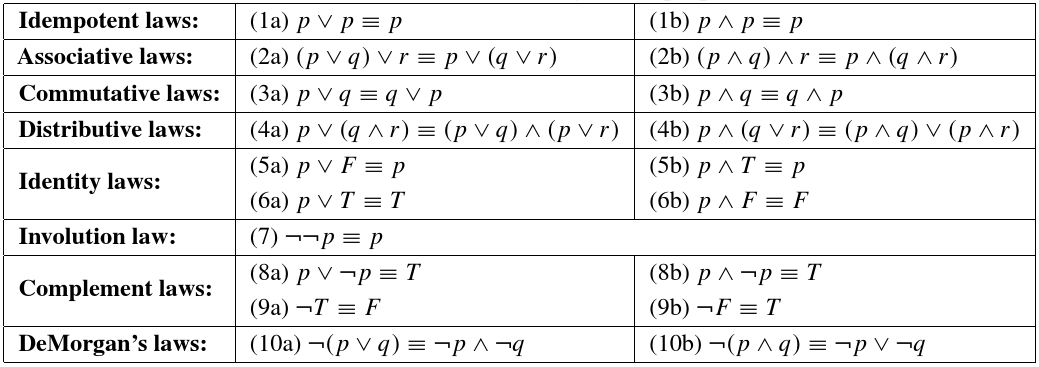
\includegraphics[width=\linewidth]{md/tabla_4-1}
 \caption{Leyes para el álgebra de proposiciones}
\label{fig:tabla:4.1}
\end{figure}



\subsection{Sentencias condicionales y bicondicionales}


 Muchas sentencias, particularmente en matemáticas, son de la forma \texttt{``si $p$ entonces $q$''}.  Tales sentencias son llamadas \emph{condicionales} y son denotadas por 
 $$
 p \imply q.
 $$ 



 El condicional $p \imply q$ es frecuentemente leído como \emph{``$p$ implica $q$''} o \emph{``$p$ sólo si $q$''.}
 \sidenote{
 \begin{tdv}[Condicional]
	\begin{center}
		\begin{tabular}{|l|l||l|} \hline
			$p$ & $q$ & $p \imply q$ \\ \hline
			$1$ & $1$ & $1$ \\ \hline
			$1$ & $0$ & $0$ \\ \hline
			$0$ & $1$ & $1$ \\ \hline
			$0$ & $0$ & $1$ \\ \hline
		\end{tabular}
	\end{center}
	
\end{tdv} 
}



 Otra sentencia común es de la forma \emph{``$p$ si y solo si $q$''.}  Tales sentencias son llamadas \emph{bicondicionales} y se denota por 
 $
 p \iff q.
 $ \sidenote{ 
 \begin{tdv}[Bicondicional]
	\begin{center}
		\begin{tabular}{|l|l||l|} \hline
			$p$ & $q$ & $p \biconditional q$ \\ \hline
			$1$ & $1$ & $1$ \\ \hline
			$1$ & $0$ & $0$ \\ \hline
			$0$ & $1$ & $0$ \\ \hline
			$0$ & $0$ & $1$ \\ \hline
		\end{tabular}
	\end{center}
	
\end{tdv} 
}







 \begin{problema}
  Demuestre que $$p\imply q \equiv \neg p \vee q.$$
 \end{problema}




 \begin{problema} Determine cuales de las siguientes sentencias son tautologías, construyendo las correspondientes tablas de verdad.
  \begin{enumerate}
   \item $\neg\left( p \vee \neg q \right) \imply \neg p$
   \item $p \imply \left( q\imply r \right)$
   \item $\left( p \imply q \right)\imply r$
   \item $\left( p\imply q \right) \imply \left( q\imply p \right)$
   \item $\left( p \wed \left( p \imply q \right) \right) \imply q$
   \item $\left( p \wed q \right) \imply p$
   \item $q \imply \left( \neg p \vee \neg q \right)$
   \item $\left( \left( p\imply q \right) \wed \left( q \imply r \right) \right) \imply \left( p \imply r \right)$
  \end{enumerate}

 \end{problema}



\subsection{Argumentos}


 Un \emph{argumento} es una afirmación de que un conjunto dado de proposiciones $$P_{1}, P_{2},...,P_{n},$$ llamadas \emph{premisas}, tiene como consecuencia otra proposición $Q,$ llamada \emph{conclusión.}\sidenote{
Por ejemplo
  \begin{center}
	\begin{tabular}{l}
		Si sube el dólar, sube la gasolina.\\
		Si sube la gasolina, entonces hay inflación.\\\hline
		$\therefore$ Si sube el dólar, entonces hay inflación.
	\end{tabular}
\end{center} 
}
 
 En otras palabras, es una sentencia de la forma
 $$
  \left( P_{1} \wed P_{2} \wed...\wed P_{n}\right) \imply Q
  $$
 
 
 
 Tal argumento se denota por $$P_{1}, P_{2},...,P_{n} \yields Q.$$



 La noción de \emph{``argumento lógico''} o \emph{``argumento válido''} se formaliza de la manera siguiente:
 
 
 \begin{definicion}
  \label{lip:4.4}
  Un argumento $P_{1}, P_{2},...,P_{n} \yields Q$ se dice que es \emph{válido} si la proposición 
  $$
  \left( P_{1} \wed P_{2} \wed...\wed P_{n}\right) \imply Q
  $$ es una tautología.
  
   Si un argumento no es \emph{válido,} diremos que es una \emph{falacia.}
 \end{definicion}




 \begin{problema}
 \label{lip:exmp:4.4}
  \begin{enumerate}
   \item Demuestre que $p, p\imply q \yields q$ es un argumento válido. 
   \item Demuestre que $p\imply q, q \yields p$ es una falacia.
   
   \item Demuestre que $p\imply q, \neg q \yields \neg p$ es un argumento válido.
  \end{enumerate}

 \end{problema}

	% TODO: \usepackage{graphicx} required
	\begin{figure}
		\centering
		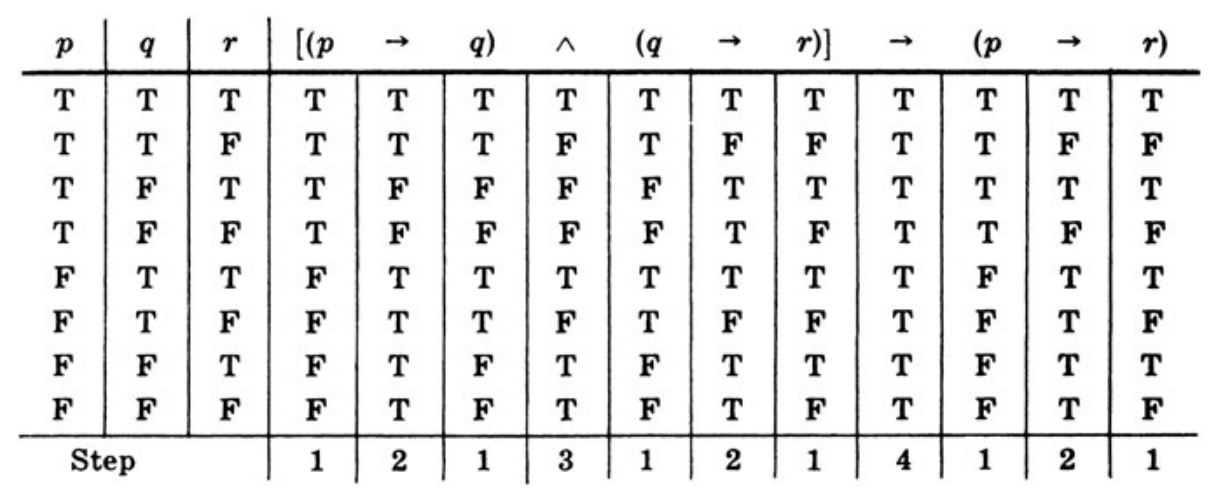
\includegraphics[width=0.7\linewidth]{md/tabla_silogismo}
		\caption{
			  Un principio fundamental del razonamiento lógico nos dice que:
				Si $p$ implica $q$ y $q$ implica $r,$ entonces $p$ implica $r.$ 
			En otras palabras, el siguiente argumento es válido
			$$
			p\imply,q, q\imply r \yields p \imply r.
			$$ }
		%\label{fig:tablasilogismo}
		\label{fig:tabla_silogismo}
	\end{figure}

\subsection{Notación de conjuntos}

Un conjunto se puede entender de forma intuitiva como una colección de objetos. Aunque la definición formal es mucho más complicada, para nuestros fines basta con esta idea sencilla.\footnote{Véase por ejemplo el artículo \href{https://www.britannica.com/science/set-theory/Axiomatic-set-theory}{Axiomatic set theory}.}

Por convención, un conjunto se puede describir de manera \emph{extensiva} escribiendo todos y cada uno de sus elementos entre paréntesis, o bien alguna característica que los defina. Por ejemplo, el conjunto de los dígitos se puede describir como
\[
	\set{\texttt{dígitos}}=\set{0,1,2,3,4,5,6,7,8,9}=\set{0,1,...,9}.
\]

	El conjunto de los números naturales está dado por
	\[ \N = \set{0,1,2,3...} ,\]	
	mientras que los números naturales están dados por 
	\[ \Z = \set{0,\pm 1, \pm 2, \pm 3...} ,\].	
	Al conjunto de enteros positivos los denotaremos por $ \Z^{+}. $
	
		Si un elemento $ x $ pertenece a un conjunto $ A $, escribiremos $ x\in A $. En caso contrario, $ x\not \in A $.

\subsection{Funciones proposicionales y Cuantificadores}


 Una \emph{función proposicional} (o \emph{sentencia abierta} o \emph{condición}) definida en un conjunto $A$ es una expresión $p(x)$ que tiene la propiedad de que $p(a)$ es cierta o falsa para cada $a \in A.$



 El conjunto $A$ se conoce como dominio de $p(x),$ y el subconjunto de todos los elementos para los cuales $p(x)$ es cierto se conoce como el \emph{conjunto de verdad} $T_{p}$ de $p(x):$
 
 $$T_{p}=\set{x \mid x\in A, p(x)=\texttt{1}},$$ 
 o simplemente 
 $$
 T_{p}=\set{x \mid p(x)}.
 $$
Esta es la manera \emph{intensiva} de describir un conjunto.



 \begin{problema}
  \label{lip:exmp:4.7}
  Encuentre el conjunto de verdad para cada función en $\N$:
  \begin{enumerate}
   \item $p(x): x+2>7$ 
   \item $p(x): x+5<3$ 
   \item $p(x): x+5>1$ 
  \end{enumerate}

 \end{problema}



\subsection{Cuantificador universal}


 Sea $p(x)$ una función proposicional definido en un conjunto $A.$ La expresión
 \[
 \label{lip:4.1}
   \forall x \in A: p(x)
 \] 
 se lee como  \texttt{``para todo $x\in A,$ $p(x)$ es verdadero.''}  
 
 El símbolo $\forall$ (\texttt{``para todo''}) se llama cuantificador universal.




 Mientras que $p(x)$ es una sentencia abierta (su valor de verdad depende de cada $x\in A$), la afirmación 
 $$\forall x\in A: p(x)$$ es verdadera si y solo si $p(x)$ se cumple para todo $x\in A.$  



 Por otro lado, si existe algún $x\in A$ tal que $p(x)$ es falso, entonces $$\forall x\in A: p(x)$$ es falso.



 \begin{problema}
  \label{lip:exmp:4.8}
  Verifique el valor de verdad de las siguientes afirmaciones:
  \begin{enumerate}
   \item $\forall n \in \N: n+4>3.$ 
   \item $\forall n \in \N: n+2>8.$
  \end{enumerate}

 \end{problema}



\subsection{Cuantificador existencial}


 Sea $p(x)$ una función proposicional definido en un conjunto $A.$ La expresión
 \[
 \label{lip:4.3}
   \exists x \in A: p(x)
 \] 
 se lee como  \texttt{``existe $x\in A,$ tal que $p(x)$ es verdadero.''}  
 
 El símbolo $\exists$ (\texttt{``existe...''}) se llama cuantificador existencial.




 Mientras que $p(x)$ es una sentencia abierta (su valor de verdad depende de cada $x\in A$), la afirmación 
 $$\exists x\in A: p(x)$$ es verdadera si y solo si $p(x)$ se cumple para algún elemento $x\in A.$  



 Por otro lado,  $$\exists x\in A: p(x)$$ es falso si y solo si para todo $ x\in A $, se tiene que $ p(x) $ es falso.



 Verifique el valor de verdad de las siguientes afirmaciones:
 \begin{enumerate}
  \item $\exists n  \in \N: n+4<7;$ 
  \item $\exists n \in \N: n+6<4.$
 \end{enumerate}



\subsection{Negación de Sentencias Cuantificadas}



 Considere la afirmación:
 \begin{center}
  \emph{Todos los estudiantes de ingeniería saben programar.}
 \end{center}
?`Cómo podemos negar esta afirmación?


\begin{center}
 \emph{Al menos un estudiante de ingeniería no sabe programar.}
\end{center} 


 De manera similar, la negación de la afirmación
 \begin{center}
  \emph{Existe algún estudiante de ingeniería que sepa programar}
 \end{center}
 es equivalente a afirmar que 
 \begin{center}
  \emph{Cada uno de los estudiantes de ingeniería no saben programar.}
 \end{center}

Estos son ejemplos de la siguiente proposición

 \begin{teorema}[DeMorgan]
  \begin{align}
  \label{lip:thm:4.4}
   \neg\left( \forall x\in M: p(x) \right)& \equiv \exists x\in M: \neg p(x)\\
   \label{lip:thm:4.5}
   \neg\left( \exists x\in M: p(x) \right)& \equiv \forall x\in M: \neg p(x).
  \end{align}

 \end{teorema}




 \begin{problema}
  \label{lip:exmp:4.10.a}
  La negación de la siguiente afirmación
  \begin{center}
   \emph{Para todo entero positivo $n,$ tenemos que $n+2>8$}
  \end{center}
es 
\begin{center}
 \emph{Existe un entero positivo $n$ tal que $n+2 \leq 8.$}
\end{center}

 \end{problema}




 \begin{problema}
  \label{lip:exmp:4.10.b}
  La negación de la siguiente afirmación
  \begin{center}
   \emph{Existe una persona viva con 150 a\~nos o más.}
  \end{center}
 es 
 \begin{center}
  \emph{Toda persona viva tiene menos de 150 a\~nos.}
 \end{center}

 \end{problema}




\marginnote{ \begin{observacion}
  Para negar una afirmación del tipo $$\forall x \in A: p(x)$$ sólo necesitamos encontrar un elemento $x_{0}\in A$ tal que $p(x)$ sea \emph{falso.}
  
  
  A un elemento $x_{0}$ así se le conoce como \emph{contraejemeplo.}
 \end{observacion}}




 \begin{problema}
 \label{lip:4.11}
  \begin{enumerate}
   \item 
  Un contraejemplo para $\forall x \in \R: \abs{x}\neq 0$ es $x=0.$  
   \item 
  Un contraejemplo para $\forall x \in \R: x^{2}\geq x$ es $x=\frac{1}{2}.$  
   \item 
  Sin embargo, $\forall x \in \N: : x^{2}\leq x$ es siempre cierto.
  \end{enumerate}

 \end{problema}





%\subsection{Bibliografía}
% Las notas de esta sección están basadas en el capítulo 4 \texttt{``Logic and Propositional Calculus''} del libro
% \begin{center}
%  \texttt{Lipschutz, S. and Lipson, M.;\textbf{ Schaum's Outline of Discrete Mathematics;} McGraw-Hill, 3th Edition.}
% \end{center}

\section*{Problemas}

%\subsection*{Proposiones y Tablas de Verdad}


\begin{problema}
	Sea $p:\texttt{``Hace frío''}$ y $q:\texttt{``Está lloviendo''.}$ Proponga un enunciado verbal simple que describa cada una de las siguientes proposiciones:
	\begin{enumerate}
		\item $\neg p;$
		\item $p \wed q;$
		\item $p \vee q;$
		\item $q \vee \neg p.$
	\end{enumerate}
	
\end{problema}




\begin{problema}
	Encuentre la tabla de verdad de $\neg p \wed q.$
\end{problema}




\begin{problema}
	Demuestre que la propisición 
	$$
	p \vee \neg \left( p\wed q \right)
	$$ es una tautología.
\end{problema}




\begin{problema}
	Muestre que las proposiciones $\neg\left( p \wed q \right)$ y $\neg p \vee \neg q$ son lógicamente equivalentes.
\end{problema}




\begin{problema}
	Use las leyes en la tabla \ref{fig:tabla:4.1} para mostrar que 
	$$
	\neg \left( p \wed q \right) \vee \left( \neg p \wed  q \right) \equiv \neg p
	$$
\end{problema}



%\subsection*{Sentencias condicionales}


\begin{problema}
	\label{lip:sol:4.6}
	Reescriba los siguientes enunciados sin usar el condicional:
	\begin{enumerate}
		\item Si hace frío, el usa sombrero. 
		\item Si la productividad se incrementa, entonces el salario aumenta.
	\end{enumerate}
	
\end{problema}




\begin{problema}
	\label{lip:sol:4.7}
	Considere la proposición condicional $p \imply q.$ La proposiciones 
	\begin{center}
		${\color{red}q \imply p,} {\color{blue}\, \neg p \imply \neg q,} \, {\color{green}\neg q \imply \neg p}$
	\end{center}
	son llamadas {\color{red} conversa,} {\color{blue}inversa} y {\color{green} contrapositiva}, respectivamente.
	
	
	?`Cuáles de estas proposiciones son lógicamente equivalente s a $p\imply q$?
\end{problema}




\begin{problema}
	Determine la contrapositiva de cada enunciado:
	\begin{enumerate}
		\item Si Erik es poeta, entonces es pobre. 
		\item Solo si Marcos estudia, pasará el examen. 
	\end{enumerate}
	
\end{problema}




\begin{problema}
	Escriba la negación de cada enunciado, tan simple como sea posible:
	\begin{enumerate}
		\item Si ella trabaja, ganará dinero. 
		\item El nada si y solo si el agua está tibia. 
		\item Si neva, entonce no manejar\'e.
	\end{enumerate}
	
\end{problema}



%\subsection*{Argumentos}


\begin{problema}
	Muestre que el siguiente argumento es una falacia:
	$$
	p\imply q, \neg p \yields \neg q.
	$$
\end{problema}




\begin{problema}
	Muestre que el siguiente argumento es válido:
	$$
	p\imply q, \neg q \yields \neg p.
	$$
\end{problema}




\begin{problema}
	Muestre que el siguiente argumento siempre es válido:
	$$
	p \imply \neg q, r \imply q, r \yields \neg p.
	$$
\end{problema}




\begin{problema}
	Determine la validez del siguiente argumento:
	\begin{center}
		\begin{tabular}{l}
			Si $7$ es menor que $4$, entonces $7$ no es número primo\\
			$7$ no es menor que $4$\\\hline
			$7$ no es número primo.
		\end{tabular}
	\end{center}
	
\end{problema}




\begin{problema}
	Determine la validez del siguiente argumento:
	\begin{center}
		\begin{tabular}{l}
			Si dos lados de un triángulo son iguales, entonces los respectivos ángulos opuestos son iguales\\
			Dos lados de un triángulo no son iguales\\\hline
			Los respectivos ángulos opuestos no son iguales.
		\end{tabular}
	\end{center}
	
\end{problema}



%\subsection*{Cuantificadores y Funciones Proposicionales}


\begin{problema}
	Sea $A=\set{1,2,3,4,5}.$ Determine el valor de verdad de cada uno de los siguientes enunciados:
	\begin{enumerate}
		\item $\exists x \in A: x+3=10;$ 
		\item $\forall x \in A: x+3<10;$ 
		\item $\exists x \in A: x+3<5;$ 
		\item $\forall x \in A: x+3 \leq 7.$
	\end{enumerate}
	
\end{problema}




\begin{problema}
	Determine el valor de verdad de cada uno de las siguientes afirmaciones donde $U=\set{1,2,3}$ es el conjunto \emph{``universo''} (de referencia):
	\begin{enumerate}
		\item $\exists x \forall y: x^{2}< y+1;$ 
		\item $\forall x \exists y: x^{2}+y^{2}<12;$ 
		\item $\forall x \forall y: x^{2}+y^{3}<12.$
	\end{enumerate}
	
\end{problema}




\begin{problema}
	Encuentre la negación de cada una de las siguientes afirmaciones:
	\begin{enumerate}
		\item $\exists x \forall y: p(x,y);$ 
		\item $\forall x \forall y: p(x,y);$ 
		\item $\exists x \exists y \forall z: p(x,y,z).$
	\end{enumerate}
	
\end{problema}




\begin{problema}
	Sea $$p(x): x+2>5.$$ Indique cuando $p(x)$ es una función proposicional o no en cada uno de los siguientes conjuntos: 
	\begin{enumerate}
		\item $\N$ 
		\item $\Z^{-}=\set{-1,-2,-3,...}$ 
		\item $\mathbb{C}$
	\end{enumerate}
	
\end{problema}




\begin{problema}
	Niegue cada uno de las siguientes afirmaciones:
	\begin{enumerate}
		\item Todos los estudiantes viven en los dormitorios.
		\item A todos los estudiantes de ingeniería le gusta el futbol.
		\item Algunos estudiantes tienen 25 años o más.
	\end{enumerate}
\end{problema}

\section{Teoría de Conjuntos}

\subsection{Conjuntos y Elementos. Subconjuntos}


	Un \emph{conjunto} puede ser visto como un conjunto bien definido de objetos, llamados \emph{elementos} o \emph{miembros} de tal conjunto. 
	
	Usualmente, usaremos letras mayúsculas para denotar conjunto, y minúsculas para dlos elementos. 



	La pertenencia en un conjunto se denota de la siguiente manera:
	\begin{center}
		\emph{$a \in S$ denota que $a$ pertenece al conjunto $S.$} 
		
		\emph{$a,b \in S$ denota que tanto $a$ como $b$ pertenecen al conjunto $S.$}
	\end{center}
	
	El símbolo $\in$ significa \texttt{``es elemento de''.}  Por el contrario, $\notin$ significa \texttt{``no es elemento de''.}


\subsection{Especificación de Conjuntos}


	Básicamente, existen dos maneras de especificar un conjunto en particular.  Por un lado, si es posible, enlistar todos los miembros.  Por otro lado, caracterizando los elementos en el conjunto.



	En cualquier caso, para declarar un conjunto se utilizan llaves:
	$$
	A=\set{\cdots}
	$$



	Por ejemplo, el conjunto 
	$$
	A=\set{1,3,5,6,9}
	$$
	tambi\'en se puede especificar como
	$$
	A=\set{x\in \N \mid x<10, 2\nmid x }
	$$



	Un conjunto no depende del modo en que sus elementos se muestren.  Este permanece igual si sus elementos se repiten o se reacomodan.




	\begin{ejemplo}
		\begin{align*}
			\set{x\in\R | x^{2}-3x+2=0} & =\set{1,2} \\
			&=\set{1,2,2,1}
		\end{align*}
		
	\end{ejemplo}
	


\subsection{Subconjuntos}


	Supongamos que cada elemento en un conjunto $A$ es tambi\'en elemento del conjunto $B,$ es decir,
	$$
	x\in A \onlyif x\in B.
	$$



	En ese caso, decimos que $A$ es subconjunto de $B.$  Tambi\'en podemos decir que $A$ está contenido en $B$ o que $B$ contiene a $A$.



	Esta relación se escribe como
	$$
	A \subset B 
	$$ o en ocasiones como
	$B\supset A.$  Por el contrario, si es necesario indicar que $A$ \emph{no} es  subconjunto de $B,$ escribimos $A \not\subset B.$



	Diremos que dos conjuntos son iguales si poseen los mismos elementos, es decir, 
	$$
	x \in A \iff x \in B.
	$$



	De manera equivalente 
	\begin{center}
		$A=B$ si y solo si $A \subset B$ y $B \subset A.$
	\end{center}
	



	\begin{ejemplo}
		\label{lip:exmp:1.2}
		Determine la relación entre los siguientes conjuntos
		\begin{center}
			$$A=\set{1,3,4,7,8,9}, \, 
			B=\set{1,2,3,4,5}, \,
			C=\set{1,3}.$$
		\end{center}
		
	\end{ejemplo}
	



	\begin{ejemplo}
		Demuestre que 
		\begin{enumerate}
			\item $A\not\subset B$ si y solo $\exists x\in A: x\notin B.$
			\item $A \subset A.$
			\item $A\subset B, B\subset C \onlyif  A\subset C.$
		\end{enumerate}
		
	\end{ejemplo}
	


\subsection{Símbolos especiales}

 Algunos conjuntos num\'ericos tienen una notación especial
	\begin{itemize}
		\item $\N:$ números naturales (enteros positivos); 
		\item $\Z:$ números enteros; 
		\item $\Q:$ números racionales; 
		\item $\R:$ números reales; 
		\item $\mathbb{C}:$ números complejos.
	\end{itemize}
	
	



	Observe que
	$$
	\N \subset \Z \subset \Q \subset \R \subset \mathbb{C},
	$$ pero en ningún caso los conjuntos son iguales. 


\subsection{Conjunto Universal y Conjunto Vacío}


	Todos los conjuntos bajo investigación en una apliación de teoría de conjuntos se supone que pertenecen a un conjunto fijo más grande llamado \emph{conjunto universo} $\uset,$ al menos que se indique otro caso.



	Dado un conjunto universal $\uset$ y una propiedad $P,$ es posible que no existan elemento de $\uset$ con la propiedad $P.$ 



	Por ejemplo, el siguiente conjunto no tiene elementos
	$$
	S=\set{x\in \Z \mid x^{2}=3}.
	$$



	A tal conjunto sin elementos $\set{}$ se le conoce como conjunto vacío y se denota como $\emptyset.$



	\begin{observacion}
		\emph{Sólo existe un conjunto vacío}.  El conjunto vacío es subconjunto de cualquier otro conjunto.
	\end{observacion}
	


\subsection{Conjuntos disjuntos}


	Dos conjuntos $A$ y $B$ son \emph{disjuntos} si no tienen elementos en común. 



	\begin{ejemplo}
		Considere $$
		A=\set{1,2}, \; B=\set{4,5,6}, \; C=\set{5,6,7,8}.
		$$
		Determine que pares de conjuntos son disjuntos. 
	\end{ejemplo}
	


\subsection{Diagramas de Venn}


	Un diagrama de Venn es una representación gráfica de conjuntos en el que cada conjunto está representado por áreas encerradas en el plano.



	El conjunto universo $\uset$ es representado por el interior de un rectángulo, y cualquier otro conjunto esta representado por discos que viven dentro del rectángulo.



	\begin{figure}
		\centering
		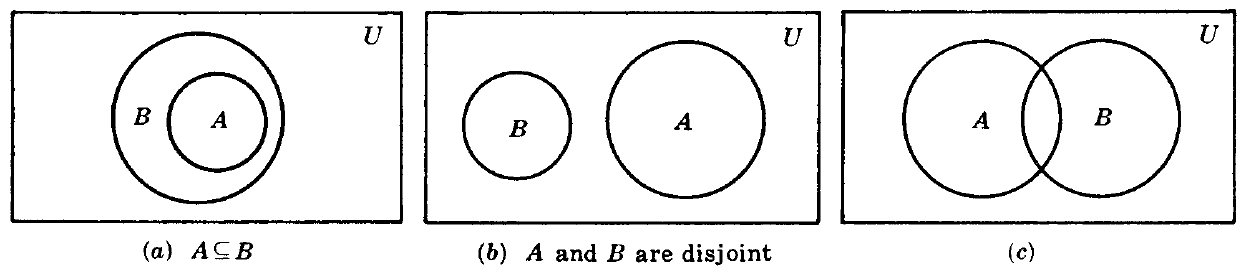
\includegraphics[width=11cm,keepaspectratio=true]{./md/venn01.png}
		% venn01.png: 0x0 pixel, 300dpi, 0.00x0.00 cm, bb=
		\caption{Representaciones con Diagramas de Venn}
		\label{fig:0101}
	\end{figure}
	


%\subsection{Operaciones con Conjuntos}
%
%
%	Sean $ A,B \subset S $. Las operaciones básicas entre conjuntos son :
%	\begin{itemize}
%		\item Unión
%		\[ A\cup B = \sett{x\in S}{x \in A \texttt{ o } x \in B} \]
%		\item Intersección
%		\[ A\cap B = \sett{x \in S}{x\in A \texttt{ y } x\in B}\]
%		\item Resta  
%		\[ A\backslash B = \sett{x\in S}{x\in A \texttt{ y } x\not \in B}\]
%		En ocasiones también denotamos la resta por $ A-B $. 
%		\item Complemento
%		\[ A' = \sett{x\in S}{x\not \in A} \]
%		A veces el complemento también se denota por $ A^{c} $ o $ \bar{A} $. De manera equivalente, se puede escribir como $ S\backslash A.$
%		\item Diferencia simétrica
%		\[ A\triangle B = \sett{x \in S}{x\in A \texttt{ o } x\in B \texttt{ pero } x\not \in A\cap B}\]. 
%	\end{itemize}


\subsection{Unión e Intersección}


	La unión de dos conjuntos $A$ y $B$ es el conjunto de todos los elementos que pertenecen a $A$ o a $B,$  es decir
	$$
	A \cup B = \set{x \mid x\in A \vee x\in B}.
	$$



	La intersección de dos conjuntos $A$ y $B$ es el conjunto de todos los elementos que pertenecen a $A$ y a $B,$  es decir
	$$
	A \cap B = \set{x \mid x\in A \wed x\in B}.
	$$



	\begin{figure}
		\centering
		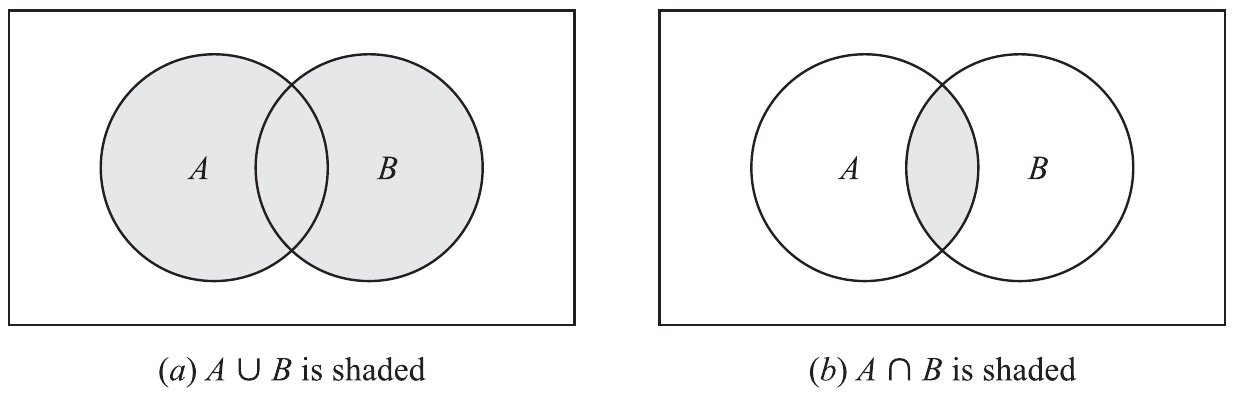
\includegraphics[width=10cm,keepaspectratio=true]{./md/venn_union_interseccion.png}
		% venn_union_interseccion.png: 0x0 pixel, 300dpi, 0.00x0.00 cm, bb=
		\caption{Unión e Intersección}
		\label{fig:0103}
	\end{figure}
	









\section*{Problemas}


\begin{problema}
	\label{lip:exmp:1.4.a}
	Sea $A=\set{1,2,3,4},$ $B=\set{3,4,5,6,7},$ $C=\set{2,3,8,9}.$ Encuentre 
	\begin{enumerate}
		\item $A \cup B=$ 
		\item $A \cap B=$ 
		\item $A \cup C=$ 
		\item $A \cap C=$ 
		\item $B \cup C=$ 
		\item $B \cap C=$
	\end{enumerate}
	
\end{problema}


\begin{problema}
	\label{thm:1.3}
	Demuestre que para cualesquiera dos conjuntos $A$ y $B,$ tenemos:
	$$
	A \cap B \subset A \subset A \cup B.
	$$
\end{problema}




\begin{problema}
	\label{thm:1.4}
	Demuestre que las siguientes proposiciones son equivalentes:
	\begin{enumerate}
		\item $\displaystyle A \subset B$
		\item $\displaystyle A \cap B = A$
		\item $\displaystyle A \cup B = B$
	\end{enumerate}
	
\end{problema}



\section{Álgebra de conjuntos}

%Dos conjuntos $A$ y $B$ se dicen \emph{disjuntos} si no tienen elementos en común, es decir $A\cap B=\emptyset$.
%
%
%Supongamos que 
%$$
%S=A\cup B, \; A\cap B=\emptyset.
%$$  Diremos que $S$ es la unión disjunta de $A$ y $B$ y se denota por $$S=A \sqcup B.$$ 



\subsection{Complementos, Diferencias y Diferencias Sim\'etricas}


En esta sección, consideraremos conjuntos que sean subconjuntos de un conjunto universo fijo $\uset.$



El \emph{complemento} $A^{C}$ de un conjunto $A$ es el conjunto de elementos que no pertenecen a $A$, es decir 
$$A^{C}=\set{x\in \uset \mid x \notin A}.$$



Algunos textos denotan $A^{C}$ tambi\'en como $A'$ o $\bar{A}.$ 



El \emph{complemento relativo} de un conjunto $B$ con respecto a un conjunto $A$ se define como 
$$
A\minus B = \set{x \mid x \in A, x \notin B}.
$$
De manera equivalente,	$A \minus B = A \cap B^{C}.$

El conjunto $A\minus B$ se lee \texttt{$A$ menos $B$.} Algunos textos lo denotan tambi\'en como $A-B.$  

La \emph{diferencia sim\'etrica} de los conjuntos $A$ y $B$ se define como $$A\symdif B=\left( A\cup B \right)\minus \left( A \cap B \right).$$



\begin{figure}
	\centering
	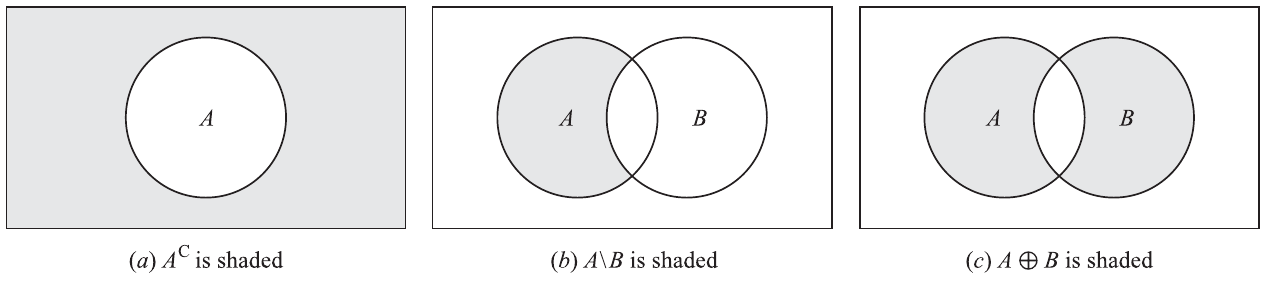
\includegraphics[width=10cm,keepaspectratio=true]{./md/venn_complemento.png}
	% venn_complemento.png: 0x0 pixel, 300dpi, 0.00x0.00 cm, bb=
	\caption{Complementos, diferencia y diferencia simétrica.}
	\label{fig:0104}
\end{figure}






\subsection{Conjuntos fundamentales}


Dos conjuntos $A$ y $B$ se dicen \emph{disjuntos} si no tienen elementos en común, es decir $A\cap B=\emptyset$.


Supongamos que 
$$
S=A\cup B, \; A\cap B=\emptyset.
$$  Diremos que $S$ es la unión disjunta de $A$ y $B$ y se denota por $$S=A \sqcup B.$$ 




En general $S$ es una unión disjunta de $P_{1}, P_{2},...,P_{n}$ si 
\begin{itemize}
	\item $\displaystyle S=P_{1}\cup P_{2}\cup...\cup P_{n}$ y
	\item $P_{i}\cap P_{j}=\emptyset$ siempre y cuando $i\neq j.$
\end{itemize}


En este caso, escribimos
$$
S=P_{1}\sqcup P_{2}\sqcup...\sqcup P_{n}.
$$



Diremos que $P_{1}, P_{2},...,P_{n}$ es sistema de conjuntos fundamentales para $\uset$ si
$$
\uset = P_{1}\sqcup P_{2}\sqcup...\sqcup P_{n}.
$$






\begin{figure}
	\centering
	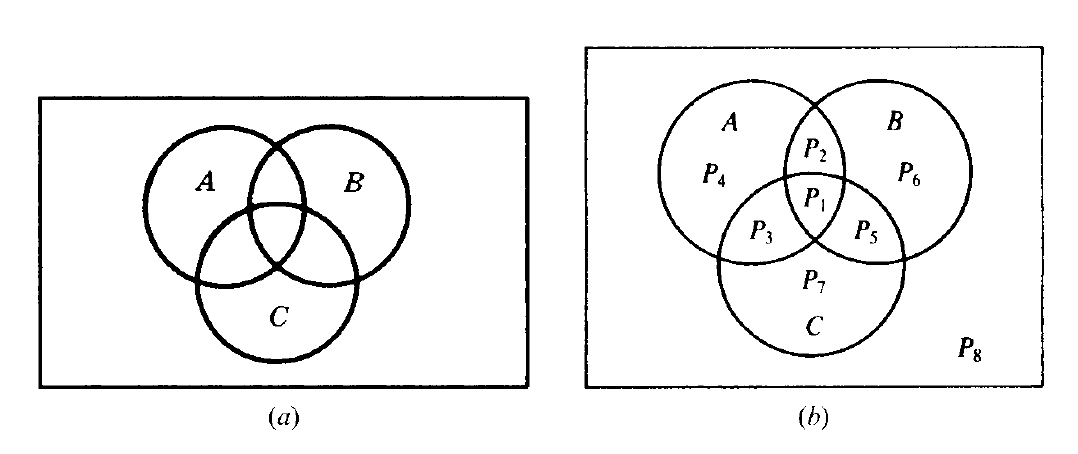
\includegraphics[width=10cm,keepaspectratio=true]{./md/sistema_fundamental.png}
	% sistema_fundamental.png: 0x0 pixel, 300dpi, 0.00x0.00 cm, bb=
	\label{fig:0105}
\end{figure}




\subsection{Álgebra de conjuntos, dualidad}


Los conjuntos bajo las operaciones de unión, intersección y complemento satisface varias leyes o identidad, que se enuncian en la siguiente tabla, y son similares a las leyes de lógica.



\begin{figure}
	\centering
	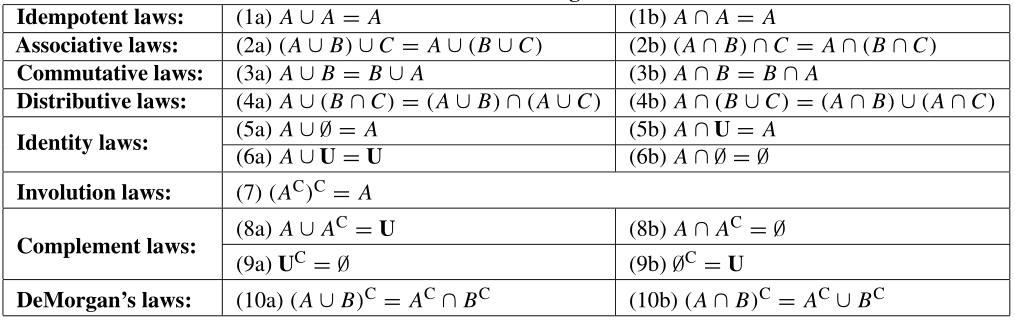
\includegraphics[width=11cm,keepaspectratio=true]{./md/leyes_conjuntos.png}
	\caption{Leyes de Conjuntos}
	\label{fig:leyesconjuntos}
\end{figure}




Cada ley de conjuntos se corresponde con una ley de lógica. Por ejemplo, la ley de DeMorgan:
\begin{align*}
	\left(A \cup B\right)^{C} &= \set{x \mid x\notin(A \cup B)}\\
	&= \set{x \mid x\notin A \wed x\notin B}\\
	&=A^{C}\cap B^{C}
\end{align*}



{Dualidad}
El \emph{principio de dualidad} establece que la equivalencia $E^{*}$ obtenida a partir de una ley de lógica $E$ reemplazando
\[ \cup, \cap, \uset, \emptyset\] por
\[ \cap, \cup, \emptyset, \uset\]
sigue siendo una ley de lógica.


A la proposición $E^{*}$ se le conoce como dual $E.$


\section*{Problemas}



\begin{problema}
	Definamos $$p\veebar q \equiv \left( p \vee q \right) \wed \neg\left( p \wed q \right)$$
	Demuestre que 
	\begin{enumerate}
		\item $ \displaystyle
		x \in A\symdif B \iff \left( x \in A \right) \veebar \left( x \in B  \right)
		$ 
		\item $\displaystyle p\veebar q \equiv \left( p \wed \neg q \right) \vee \left( q \wed \neg p \right)$ 
		\item $\displaystyle A \veebar B = \left( A \minus B \right) \cup \left( B \minus A \right)$
	\end{enumerate}
	
\end{problema}

\begin{problema}
	\label{lip:exmp:1.5}
	Supongamos que $\N$ es el conjunto universo. Definamos $A=\set{1,2,3,4},$ $B=\set{3,4,5,6,7},$ $C=\set{2,3,8,9},$ $E=\set{2,4,6,...}.$
	
	Determine:
	\begin{enumerate}
		\item $A \symdif B$ 
		\item $A \symdif C$ 
		\item $B \symdif C$ 
		\item $A \symdif E$
	\end{enumerate}
\end{problema}


\begin{problema}
	\label{lip:exmo:1.6}
	Contruya un sistema de conjuntos fundamentales a partir de tres conjunto $A, B, C.$  
\end{problema}


\begin{problema}
	Encuentre el dual de 
	\[ (\uset \cap A) \cup (B\cap A) = A\]
\end{problema}
\section{Relaciones}


	{Ejemplos de relaciones}
	\begin{itemize}
		\item ``menor que''
		\item ``es paralelo a''
		\item ``es un subconjunto de''
	\end{itemize}
	



	Formalmente, definiremos una relación en t\'erminos de \emph{pares ordenados.}



	\begin{definicion}
		Un \emph{par ordenado} de elementos $a$ y $b,$ donde $a$ es el primer elemento y $b$ es el segundo se denota por $(a,b).$
	\end{definicion}
	



	
	\begin{ax}
		$(a,b)=(c,d)$  si y sólo si $a=c$ y
		$b=d.$
	\end{ax}
	
	
	
	En particular $(a,b)\neq(b,a),$  al menos que $a=b.$
	
	
	
	Esto es muy diferente al caso de un conjunto, dónde el orden es irrelevante:
	$$
	\set{a,b}=\set{b,a}.
	$$


\subsection{Producto de conjuntos}


	Consideremos dos conjuntos arbitrarios $A$ y $B.$ El conjunto de todos los pares ordenadors $(a,b)$ donde $a\in A, b \in B$ es llamado \emph{producto(cartesiano)} de $A$ con $B,$ y se denota por $A \times B,$ es decir,
	$$
	A \times B = \set{(a,b) \mid a \in A, \; b \in B}
	$$



	Podemos construir el producto cartesiano de un conjunto $A$ consigo mismo, y en ese caso denotaremos
	$$A^{2}= A\times A.$$



	\begin{problema}
		Sea $A=\set{x,y}, \, B={0,1}.$ Entonces
		\begin{enumerate}
			\item $A^{2}=\set{(x,x), (x,y), (y,x), (y,y)}$
			\item $A\times B= \set{(x,0), (x,1), (y,0), (y,1)}$
			\item $B\times A= \set{(0,x), (0,y), (1, x), (1,y)}$
			\item $B^2=\set{(0,0), (0,1), (1,0), (1,1)}$
		\end{enumerate}
		
	\end{problema}
	



	\begin{observacion}
		\begin{itemize}
			\item En general, $A\times B \neq B \times A.$
			\item Si \emph{$n(A)$} denota el \emph{número de elementos} en el conjunto $A,$ entonces
			$$
			n(A \times B)= n(A) \cdot n(B).
			$$
		\end{itemize}
		
	\end{observacion}
	




	Sean $A=\set{1,2}$ y $B={a,b,c}.$ Determine $A\times B,$ $B\times A$ y $A^{2},$ y describa gráficamente estos productos.



	\begin{problema}
		$\R^{2}=\R \times \R$ es llamado frecuentemente el \emph{plano Cartesiano.}
	\end{problema}
	



	\begin{definicion}
		Definimos el producto cartesiano de un número finito de conjuntos $A_{1},...,A_{n}$ como
		$$
		\prod_{i=1}^{n} A_{i}= A_{1} \times \cdots \times A_{n}=\set{\left( a_{1},\dots,a_{n} \right)\mid a_{1}\in A_{1}, \dots, a_{n}\in A_{n}}
		$$
	\end{definicion}
	



	\begin{observacion}
		De manera análoga al caso $n=2,$ definiremos
		$$
		A^{n}=\prod_{i=1}^{n}A.
		$$
		
		
		Por ejemplo, $\R^{3}$ denota el espacio tridimensional.
	\end{observacion}
	


\subsection{Relaciones}


	\begin{definicion}
		Sean $A$ y $B$ conjuntos arbitrarios. Una \emph{relación binaria $R$,} o simplemente relación, de $A$ a $B$ es un subconjunto de $A \times B.$
	\end{definicion}
	



	Para cada $(a,b)\in A \times B$ alguna de las siguientes condiciones (pero no ambas) es cierta:
	\begin{enumerate}
		\item $(a,b)\in R;$ en cuyo caso diremos que \emph{$a$ está $R-$relacionado con $b$,} y escribiremos $a \rel{R} b.$
		\item $(a,b)\not\in R;$ en cuyo caso diremos que \emph{$a$ no está $R-$relacionado con $b$,} y escribiremos $a \nrel{R} b.$
	\end{enumerate}
	



	Si $R$ es una relación de $A$ en sím mismo, es decir $R \subset A^{2},$ entonces diremos que $R$ es una \emph{relación en $A$.}



	\begin{definicion}
		Si $R \subset A \times B$ es una relación, el \emph{domino de $R$} es 
		$$
		\dominio{R}=\set{a\in A\mid (a,b)\in R},
		$$ mientras que la \emph{imagen de $R$} es 
		$$
		\imagen{R}=\set{b\in B\mid (a,b)\in R}.
		$$
	\end{definicion}
	


\subsection{Ejemplos}

	Sean $A=\set{1,2,3},$ $B=\subset{x,y,z}$ y $$R=\set{(1,y), (1,z), (3,y)}.$$ Entonce $R$ es una relación de $A$ en $B,$ porque $R \subset A \times B.$
	
	
	Respecto a esta relación, por ejemplo,
	$$
	1\rel{R}y, \; 1\rel{R}z, \; 3\rel{R}y,
	$$ pero 
	$$
	1\nrel{R}x, 2\nrel{R}x, 2\nrel{R}y.
	$$
	
	
	En este caso, $\dominio{R}=\set{1,3}$ e $\imagen{R}=\set{y,z}.$



	La propia inclusión $\subset$ es una relación en una colección de conjuntos $A_{1},...,A_{n}.$ 
	
	Para cualquier par $A_{i}, A_{j}$ en dicha colección $A \subset B$ o $A \not\subset B.$



	Una relación en el conjunto $\Z$ de número enteros es \emph{\texttt{``$m$ divide a $n.$''}}
	
	
	La notación convencional para esta relación es \emph{$m \mid n.$}



	Consideremos el conjunto de lineas $L$ en el plano. La perpendicularidad $\perp$ es una relación en $L.$  De manera similar el paralelismo $\parallel.$



	Sea $A$ cualquier subconjunto. Una relación importante en $A$ es la \emph{igualdad}
	$$
	\set{(a,a) \mid a \in A}
	$$ que usualmente se denota por \emph{$$``=''$$} 
	 En ocasiones, tambi\'en se le llama \emph{entidad} o \emph{diagonal} y se denota por $\triangle_{A},$ o simplemente por $\triangle.$



	Sea $A$ un conjunto arbitrario. Entonces tanto $A\times A$ como $\emptyset$ son subconjuntos de $A \times A,$ y son llamados \emph{relación universal} y \emph{relación vacía,} respectivamente.



	{Relación inversa}
	
	Sea $R$ una relación de $A$ en $B.$ La \emph{relación inversa} de $R,$ denotada por \emph{$R^{-1}$,} es la relación de $B$ en $A$ que consiste en todos aquellos pares que al invertirlos, pertenecen a $R.$ 
	
	En otras palabras
	$$
	R^{-1}=\set{(b,a)\mid (a,b)\in R}.
	$$



	\begin{problema}
		Sea $A=\set{1,2,3}, B=\set{x,y,z}$ y $R=\set{(1,y),(1,z),(3,y)}.$ Entonces
		$$
		R^{-1}=\set{(y,1), (z,1), (y,3)}.
		$$
	\end{problema}



	\begin{observacion}
		\begin{itemize}
			\item $\left( R^{-1} \right)^{-1}=R.$
			\item $\dominio{R^{-1}}=\imagen{R}$
			\item $\imagen{R^{-1}}=\dominio{R}$
		\end{itemize}
	\end{observacion}




\subsection{Composición de Relaciones}

	Sean $A,B,C$ conjuntos arbitrarios, $R$ una relación de $A$ en $B$ y $S$ una relación de $B$ en $S.$  Entonces podemos definir una nueva relación de $A$ en $C$ denotada por \emph{$RS$:}
	\begin{center}
		$a\rel{{RS}}c$ si para alguna $b \in B,$ $a\rel{R}b$ y $b\rel{S}c.$
	\end{center} 



	Esto es
	$$
	RS=\set{(a,c)\mid \exists b\in B: (a,b)\in R, (b,c)\in S}
	$$



	Supongamos que $R$ es una relación en $A.$ Entonces, definimos $R^{n}$ de manera recursiva
	$$
	R^{1}=
	\begin{cases}
		R & n=1 \\
		R^{n-1}R & n>1
	\end{cases}
	$$




	



	\begin{teorema}
		Supongamos que $R$ es uan relación de $A$ en $B,$ y $S$ una relación de $B$ en $C.$ Entonces
		$$
		(RS)T=R(ST).
		$$
	\end{teorema}
	


\subsection{Tipos de relaciones}

\paragraph{Relaciones reflexivas}


	
	Una relación $R$ es un conjunto $A$ es \emph{reflexiva} si $a\rel{R}a$ para todo $a\in A$, \, es decir, $\forall a \in A: (a,a)\in \R.$ 
	



\paragraph{Relaciones sim\'etricas y antisim\'etricas}


	Una relación $R$ en un conjunto $A$ es sim\'etrica si: Siempre que $a\rel{R}b,$ entonces $b\rel{R}a.$  En otras palabras, 
	$$
	(a,b)\in \R \onlyif (b,a)\in \R.
	$$





	Una relación $R$ en un conjunto $A$ es antisim\'etrica si: Siempre que $a\rel{R}b$ y $b\rel{R}a$ entonces $a=b.$  En otras palabras, 
	$$
	a\neq b, a\rel{R}b \onlyif b\nrel{R}a.
	$$
	


	\begin{observacion}
		Las propiedades de simetría y antisimetría no son excluyentes una de la otra. 
		
		Por ejemplo, la relación $$R=\set{(1,3),(3,1),(2,3)}$$ no es sim\'etrica ni antisim\'etrica. 
		
		Por otro lado, la relación $$S=\set{(1,1),(2,2)}$$ es tanto sim\'etrica como antisim\'etrica.
	\end{observacion}
	


\paragraph{Relación transitiva}


	Una relación $R$ en un conjunto $A$ es transitiva si: Siempre que $a\rel{R}b$ y $b\rel{R}c,$ entonces $a\rel{R}c.$  En otras palabras, 
	$$
	(a,b)\in R, (b,c)\in R \onlyif (a,c)\in \R.
	$$
	
	


 \paragraph{Propiedades de cerradura}
 
 
 Consideremos un conjunto dado $A$ y la colección de todas las relaciones en $A,$ y sea $P$ una propiedad en la colección de tales relaciones, por ejemplo, la simetría o la transitividad.
 
 
 Si una relación satisface la propiedad $P,$ diremos que es una $P-$relación.
 

\subsection{Relaciones de Equivalencia}

	Considere un conjunto no-vacío $S.$ Una relación $R$ en $S$ es una \emph{relación de equivalencia} si $R$ es reflexiva, sim\'etrica y transitiva.



	En otras palabras, $R$ es una \emph{relación de equivalencia} en $S$ si satisface las siguientes propiedades:
	\begin{enumerate}
		\item Para cada $a\in S:$ $a\rel{R}a;$
		\item si $a\rel{R}b,$ entonces $b\rel{R}a;$
		\item si $a\rel{R}b,$ $b\rel{R}c,$ entonces $a\rel{R}c.$
	\end{enumerate}
	



	La idea general detras de una relación de equivalencia que es una clasificación de objetos que son en cierto sentido \emph{similares.} 
	
	
	Por ejemplo, la relación \emph{$=$} de igualdad en cualquier conjunto $S$ es una relación de equivalencia, porque...



	\begin{problema}
		\label{lip:exmp:2.12.a}
		Sea $L$ el conjunto de líneas en el plano cartesiano y $T$ el conjunto de triangulos en el mismo plano.
		
		\begin{enumerate}
			\item La relación de paralelidad es una relación de equivalencia en $L;$ 
			\item La relación de congruencia o la de similaridad son relaciones de equivalencia en $T.$
		\end{enumerate}
		
	\end{problema}
	


	\label{lip:exmp:2.12.c}
	Sea $m$ un entero positivo fijo. Dos enteros $a,b$ son llamados \emph{congruentes módulo $m,$} si $m$ divide la diferencia $a-b,$ y en tal caso escribimos:
	$$
	a\equiv b \mod m.
	$$
	
	
	Por ejemplo $11\equiv 3 \mod 4$ y $22\equiv 6 \mod 4.$
	
	
	La relación de congruencia módulo $m$ es un relación de equivalencia. 



\subsection{Particiones y clases de equivalencia}


	Una paritición $P$ de un conjunto no-vacío $S$ es una colección $\set{A_{j}}$de subconjuntos no-vaciós de $S$ con las siguientes propiedades de que cada $a\in S$ pertenece a uno y solo uno de los conjunto $A_{j}$ de la partición.  
	
	En otras palabras,
	\begin{enumerate}
		\item Cada $a\in S$ pertenece a algún $A_{j};$
		\item si $A_{i}\neq A_{j},$ entonces $A_{j}\cap A_{j}=\emptyset.$
		
	\end{enumerate}
	
	
	De manera equivalente, una partición $P$ de $S$ es una subdivisión de $S$ en conjuntos disjuntos no vacíos $A_{j}$ tal que $$S= \sqcup_{j} A_{j}.$$



	Supontamos que $R$ es una relación de equivalencia en el conjunto $S.$ Para cada $a\in S,$ denotemos por $[a]$ el conjunto de elementos de $S$ tales que están $R-$relacionados con $a.$ 
	
	
	En otras palabras,
	$$
	[a]=\set{x \in S \mid (a,x)\in R}.
	$$



	La colección de clases de equivalencia de elementos de $S$ bajo una relación de de equivalencias $R$ se denota por $S/R,$ es decir,
	$$
	S/R=\set{[a] \mid a \in S}.
	$$
	 
	
	Diremos que $S/R$ es el conjunto cociente de $S$ por $R.$



	\begin{teorema}
		\label{lip:thm:2.6}
		Sea \emph{$R$ una relación de equivalencia en $S.$} Entonces \emph{S/R es una partición de $S.$} 
		De manera especifica:
		\begin{enumerate}
			\item Para cada $a \in S:$  $a\in [a];$
			\item $[a]=[b]$ si y solo si $(a,b)\in R;$
			\item Si $[a]\neq [b],$ entonces $[a]$ y $[b]$ son conjuntos disjuntos. 
		\end{enumerate}
		
		
		De manera inversa, dada una partición $P=\set{A_{j}}$ de conjuntos $S,$ existe una relación $R$ en $S$ tal que los conjuntos $A_{j}$ son las clases de de equivalencia de $R.$
	\end{teorema}
	



	\begin{problema}
		\label{lip:exmp:2.13.b}
		Sea $R=\set{(1,1),(1,2),(2,1),(2,2),(3,3)}$ en $S=\set{1,2,3}.$ Demuestre que $R$ es una relación de equivalencia y calcule $S/R.$
	\end{problema}
	






\paragraph{Relaciones de orden parcial}


	Una relación $R$ en un conjunto $S$ es llamada \emph{orden parcial} de $S$ en $R$ si es reflexiva, antisim\'etrica y transitiva. 
	
	Un conjunto $S$ con un orden parcial $R$ es llamado \emph{conjunto parcialmente ordenado} o \emph{poset.}
\section*{Problemas}

\begin{problema}
Sea $A=\set{1,2,3,4},$ $B=\set{a,b,c,d}$ y $C=\set{x,y,z}$ y definimos las relaciones: 
$$R=\set{(1,a),(2,d),(3,a),(3,b),(3,d)}$$  $$S=\set{(b,x),(b,z),(c,y),(d,z)}.$$ Encuentre $RS.$
\end{problema}

	\begin{problema}
	Determine cuando una relación $R$ es \emph{no-reflexiva}.
\end{problema}

\begin{problema}
	\label{lip:exmp:2.5}
	Sea $A=\set{1,2,3,4}.$ Determine cuales de las siguientes relaciones son reflexivas:
	\begin{itemize}
		\item $R_{1}=\set{(1,1),(1,2),(2,3),(1,3),(4,4)}$ 
		\item $R_{2}=\set{(1,1),(1,2),(2,1),(2,2),(3,3),(4,4)}$ 
		\item $R_{3}=\set{(1,3),(2,1)}$
		\item $R_{4}=\emptyset$
		\item $R_{5}=A \times A$
	\end{itemize}
	
\end{problema}




\begin{problema}
	\label{lip:exmp:2.6}
	Determine cuales de las siguientes relaciones son reflexivas:
	\begin{itemize}
		\item $\leq$ en $\Z$ 
		\item $\subset$ en $2^{A}$ 
		Aquí $A$ es un conjunto y $2^{A}$ es la colección de todos sus subconjuntos (incluyendo tanto a $\emptyset$ como $A$) 
		\item $\perp$ en el conjunto $L$ de líneas en el plano 
		\item $\parallel$ en el conjunto $L$ de líneas en el plano 
		\item $\mid$ (divisivilidad) en $\N.$  Aquí $a\mid b$ significa que \emph{a divide a b.} 
	\end{itemize} 
\end{problema}

	
\begin{problema}
	Determine cuando una relación $R$ no es sim\'etrica.
\end{problema}




\begin{problema}
	\label{lip:exmp:2.7}
	\begin{enumerate}
		\item   Determine cuales de las relaciones en el ejemplo \ref{lip:exmp:2.5} son sim\'etricas.
		\item Determine cuales de las relaciones en el ejemplo \ref{lip:exmp:2.6} son sim\'etricas.
	\end{enumerate}
	
\end{problema}


\begin{problema}
	Determina cuando una relación $R$ no es sim\'etrica.
\end{problema} 


\begin{problema}
	\label{lip:exmp:2.8}
	\begin{enumerate}
		\item   Determine cuales de las relaciones en el ejemplo \ref{lip:exmp:2.5} son antisim\'etricas.
		\item Determine cuales de las relaciones en el ejemplo \ref{lip:exmp:2.6} son antisim\'etricas.
	\end{enumerate}
	
\end{problema}


\begin{problema}
	Determina cuando una relación $R$ no es transitiva.
\end{problema}




\begin{problema}
	\label{lip:exmp:2.9}
	\begin{enumerate}
		\item   Determine cuales de las relaciones en el ejemplo \ref{lip:exmp:2.5} son transitivas.
		\item Determine cuales de las relaciones en el ejemplo \ref{lip:exmp:2.6} son transitivas.
	\end{enumerate}
	
\end{problema}



\begin{problema}
	\label{lip:exmp:2.12.b}
	La relación $\subset$ no es una relación de equivalencia. Demuestra que aunque es reflexiva y transitiva,  no es sim\'etrica. 
\end{problema}



\begin{problema}
	Para cada relación, verifique que se trata de una relación de equivalencia, y calcule sus clases de equivalencia.
\end{problema}

\begin{itemize}
	\item $\displaystyle R_{0}= \left[\left[\text{\texttt{a}}, \text{\texttt{a}}\right], \left[\text{\texttt{b}}, \text{\texttt{b}}\right], \left[\text{\texttt{c}}, \text{\texttt{c}}\right]\right] $
	\item $\displaystyle R_{1}= \left[\left[\text{\texttt{a}}, \text{\texttt{a}}\right], \left[\text{\texttt{a}}, \text{\texttt{b}}\right], \left[\text{\texttt{b}}, \text{\texttt{a}}\right], \left[\text{\texttt{b}}, \text{\texttt{b}}\right], \left[\text{\texttt{c}}, \text{\texttt{c}}\right]\right] $
	\item $\displaystyle R_{2}= \left[\left[\text{\texttt{a}}, \text{\texttt{a}}\right], \left[\text{\texttt{a}}, \text{\texttt{c}}\right], \left[\text{\texttt{b}}, \text{\texttt{b}}\right], \left[\text{\texttt{c}}, \text{\texttt{a}}\right], \left[\text{\texttt{c}}, \text{\texttt{c}}\right]\right] $
	\item $\displaystyle R_{3}= \left[\left[\text{\texttt{a}}, \text{\texttt{a}}\right], \left[\text{\texttt{b}}, \text{\texttt{b}}\right], \left[\text{\texttt{b}}, \text{\texttt{c}}\right], \left[\text{\texttt{c}}, \text{\texttt{b}}\right], \left[\text{\texttt{c}}, \text{\texttt{c}}\right]\right] $
	\item $\displaystyle R_{4}= \left[\left[\text{\texttt{a}}, \text{\texttt{a}}\right], \left[\text{\texttt{a}}, \text{\texttt{b}}\right], \left[\text{\texttt{a}}, \text{\texttt{c}}\right], \left[\text{\texttt{b}}, \text{\texttt{a}}\right], \left[\text{\texttt{b}}, \text{\texttt{b}}\right], \left[\text{\texttt{b}}, \text{\texttt{c}}\right], \left[\text{\texttt{c}}, \text{\texttt{a}}\right], \left[\text{\texttt{c}}, \text{\texttt{b}}\right], \left[\text{\texttt{c}}, \text{\texttt{c}}\right]\right] $
	
\end{itemize}





\begin{problema}
	\label{lip:exmp:2.13.b}
	Describa las clases de equivalencia de $\Z \mod 5,$ y verifique que las operaciones
	$$
	[a]+[b]=[a+b], \; [a]\cdot[b]=[a \cdot b]
	$$ están bien definidas.   
\end{problema}





\begin{problema}
	Considere el conjunto $S=\set{(a,b)\in \Z^{2}\mid b\neq0}$ y la siguiente relación en este conjunto
	$
	(a,b)\rel{R}(c,d) \iff ad-bc=0.
	$
	
	\begin{enumerate}
		\item Demuestre que $R$ es una relación de equivalencia.
		\item Demuestre que $[(a,b)]=[(c,d)]$ para todo $n\in\Z, n \neq 0$
		$$
		[(a,b)]=[(n\cdot a, n\cdot b)]
		$$
		\item Demuestre que las operaciones
		$$
		\begin{cases}
			[(a,b)]+[(c,d)]=[(ad+bc,bd)] \\
			[(a,b)]\cdot[(c,d)]=[(a\cdot c, b \cdot d)]
		\end{cases}
		$$ están bien definidas
		\item Denote por $\frac{a}{b}$ la clase de equivalencia $[(a,b)]$ y reescriba los resultados anteriores usando esta notación.
		\item ?`Qu\'e conjunto de números representa el cociente $S/R.$?
	\end{enumerate}
\end{problema}



\begin{problema}
	Para cada una de las siguientes relaciones, verifique que es un orden parcial y dibuje su diagrama de Hasse.
\end{problema}
\begin{itemize}
	\item $\displaystyle R_{1}= \left[\left[\text{\texttt{a}}, \text{\texttt{a}}\right], \left[\text{\texttt{b}}, \text{\texttt{b}}\right], \left[\text{\texttt{c}}, \text{\texttt{c}}\right]\right] $
	\item $\displaystyle R_{2}= \left[\left[\text{\texttt{a}}, \text{\texttt{a}}\right], \left[\text{\texttt{a}}, \text{\texttt{b}}\right], \left[\text{\texttt{b}}, \text{\texttt{b}}\right], \left[\text{\texttt{c}}, \text{\texttt{c}}\right]\right] $
	\item $\displaystyle R_{3}= \left[\left[\text{\texttt{a}}, \text{\texttt{a}}\right], \left[\text{\texttt{a}}, \text{\texttt{c}}\right], \left[\text{\texttt{b}}, \text{\texttt{b}}\right], \left[\text{\texttt{c}}, \text{\texttt{c}}\right]\right] $
	\item $\displaystyle R_{4}= \left[\left[\text{\texttt{a}}, \text{\texttt{a}}\right], \left[\text{\texttt{a}}, \text{\texttt{b}}\right], \left[\text{\texttt{a}}, \text{\texttt{c}}\right], \left[\text{\texttt{b}}, \text{\texttt{b}}\right], \left[\text{\texttt{c}}, \text{\texttt{c}}\right]\right] $
	\item $\displaystyle R_{6}= \left[\left[\text{\texttt{a}}, \text{\texttt{a}}\right], \left[\text{\texttt{b}}, \text{\texttt{b}}\right], \left[\text{\texttt{b}}, \text{\texttt{c}}\right], \left[\text{\texttt{c}}, \text{\texttt{c}}\right]\right] $
	\item $\displaystyle R_{7}= \left[\left[\text{\texttt{a}}, \text{\texttt{a}}\right], \left[\text{\texttt{a}}, \text{\texttt{c}}\right], \left[\text{\texttt{b}}, \text{\texttt{b}}\right], \left[\text{\texttt{b}}, \text{\texttt{c}}\right], \left[\text{\texttt{c}}, \text{\texttt{c}}\right]\right] $
	\item $\displaystyle R_{8}= \left[\left[\text{\texttt{a}}, \text{\texttt{a}}\right], \left[\text{\texttt{a}}, \text{\texttt{b}}\right], \left[\text{\texttt{a}}, \text{\texttt{c}}\right], \left[\text{\texttt{b}}, \text{\texttt{b}}\right], \left[\text{\texttt{b}}, \text{\texttt{c}}\right], \left[\text{\texttt{c}}, \text{\texttt{c}}\right]\right] $
\end{itemize}




\begin{problema}
	\label{lip:exmp:2.14}
	Demuestre para cada par $(S,R),$ el conjunto $S$ es parcialmente ordenado respecto a $R:$
	\begin{enumerate}%
		\item $(2^{A}, \subset).$ %Aquí $A$ denota un conjunto arbitrario y $2^{A}$ la colección de todos sus subconjuntos.
		
		\item $(\R, \leq )$
		\item $(\N, \mid).$  Muestre que esto no es cierto para $(\Z, \mid).$
	\end{enumerate}
	
\end{problema}


\chapter{Combinatoria}
\section{Funciones}

\subsection{Funciones, gráficas y relaciones}

Supongamos que para cada elemento de un conjunto $A,$ asignamos un \emph{único} elemento de un conjunto $B;$ diremos que la colección de tales asignaciones es una \emph{función} de $A$ en $B.$ 


En tal caso, denotamos escribimos 
$$f:A\to B, \; a \mapsto f(a)$$
donde $f(a)\in B$ es la asignación correspondiente a $a\in A.$



La conexión entre \emph{funciones} y \emph{relaciones} es la siguiente:


Definimos la gráfica de una función $f:A\to B$ como el subconjunto de $A \times B$
$$
\Gamma_{f}=\set{(a, f(a)) \mid a \in A}.
$$


 $f:A\to B$ es una función si su gráfica es una relación tal que $$(a,b), (a,b')\in \Gamma_{f} \onlyif b=b'.$$  
\emph{Observe que $\Gamma_{f}$ es una relación en $A\times B.$}

En este caso, diremos que $a\in A$ es la \emph{varible independiente,} mientras que $b\in B$ es la \emph{variable dependiente.}



De manera reciproca, una relación $R\subset A \times B$ induce una función si 
$$
(a,b), (a,b')\in R \onlyif b=b'.
$$


En tal caso (abusando de la notación), la función está definida por 
$$
R:A\to B, \; a \mapsto b:=R(a).
$$



Entonces, una relación no induce una función si...


El conjunto $A$ es llamado \emph{dominio} de la función, y al conjunto $B$ se le conoce \emph{codominio.}


La \emph{imagen} de una función $f:A\to B$ se define como
\begin{align*}
	\imagen{f}&=f(A)\\
	&=\set{b \in B : \exists a \in A, b=f(a)}\\
	&=\set{f(a)\in B : a \in A}
\end{align*}

Frecuentemente, una función puede expresarse por medio de una fórmula matemática. 
\begin{problema}
	Consideremos la función que asigna a cada número real su cuadrado. Podemos describir esta función escribiendo
	$$
	f(x)=x^{2} \texttt{ o } x\mapsto x^{2} \texttt{ o } y=x^{2}.
	$$
\end{problema}



En el ejemplo anterior, la gráfica de $f:\R \to \R$ esta dada por 
$$
\Gamma_{f}=\set{(x,y)\in \R^{2}\mid y=x^{2}}
$$ y es una parábola.


Mientras que la imagen de $f$ esta dada por 
$$
f(\R)=\set{x^{2}\mid x\in \R}=\set{y\in \R \mid y\geq 0}.
$$



\begin{problema}
	La relación 
	$$
	R=\set{(x,y)\in \R^{2}\mid x^{2}+y^{2}=1}
	$$
	no induce una función.
\end{problema}




\begin{problema}
	Sea $A$ un conjunto arbitrario. La función $:A \to A$ que asigna a cada elemento $a\in A$ el mismo elemento es llamada \emph{identidad,} usualmente denotada por $\id_{A}$ o simplemente $\id$
	
	
	En otras palabras, la identidad está definida por $$
	\id:A\to A, \; a \mapsto \id(a)=a.
	$$ Observe que
	$$
	\Gamma_{\id_{A}}=\triangle_{A}.
	$$
\end{problema}



 
 \begin{problema}
  Supongamos que $S \subset A.$ La \emph{inclusión} de $S$ en $A,$ denotada por $i: S \hookrightarrow A$ esta dada por $i(x)=x.$
 
 
 Observe que es la asignación es similar a la identidad, pero el dominio está restringido a $S \subset A.$
 
 
 La \emph{restricción} $f\mid_{S}$ de una función $f:A \to B$ a $S \subset A$ esta dada por
 $$
 f\mid_{S}: S \to B, \; x\mapsto f(x).
 $$
 \end{problema}
 
 

\subsection{Composición de Funciones}


Consideremos dos funciones $f:A \to B$ y $g:B \to C.$ Podemeos definir una nueva función $:A \to C$ de la siguiente manera
$$
a \mapsto {\color{purple}b=f(a)} \mapsto c=g({\color{purple}b})=g({\color{purple}f(a)}).
$$


La función anterior se conoce como \emph{composición} $g$ con se $f$ se describe de la siguiente manera
$$
\begin{cases} 
	{\color{red} g\circ f}:A\to C \\ 
	x \mapsto {\color{purple}g(f(x))}.
\end{cases}
$$




\subsection{Funciones inyectivas, suprayectivas e inversas}


\begin{definicion} Consideremos una función $f:A\to B.$ Diremos que
	\begin{enumerate}
		\item $f$ es \emph{inyectiva} o \emph{1:1} si $\displaystyle f(a)=f(a')\onlyif a=a'.$ 
		
		\item $f$ es \emph{suprayectiva} o \emph{sobre} si
		$\displaystyle f(A)=B.$ 
		
		\item $f$ es \emph{biyectiva} o \emph{invertible} si la relación inversa de la gráfica $\Gamma_{f}$ induce una función. 
	\end{enumerate}
	
\end{definicion}



\begin{proposicion}
	La función $f:A\to B$ es invertible si y solo si es $1:1$ y sobre.  
	
	En tal caso la relación inversa $R^{-1}$ de $R=\Gamma_{f}$ induce una función denotada por $\displaystyle f^{-1}:B\to A$ tal que
	$$
	\begin{cases}
		f^{-1} \circ f = \id_{A}\\
		f \circ f^{-1} = \id_{B}
	\end{cases}
	$$
\end{proposicion}






\subsection{Como encontrar funciones inversas}


Si $f:A \to B$ no es \emph{sobre,} es decir, $f(A) \subset B$ pero $f(A)\neq B,$ basta restringir su codominio a la imagen $f(A)$ para que se convierta en {sobre}:
$$
f: A \to f(A).
$$



\begin{problema}
	La función $f:\R \to \R, x \mapsto x^{2}$ no es sobre, pero como 
	$$f(A)=\set{x^2\mid x\in\R}=\set{y\in \R \mid y\geq 0}$$
	la función $f: \R\to \set{y \geq 0}, x \mapsto x^{2}$ sí lo es.
\end{problema}




\begin{figure}
	\centering
	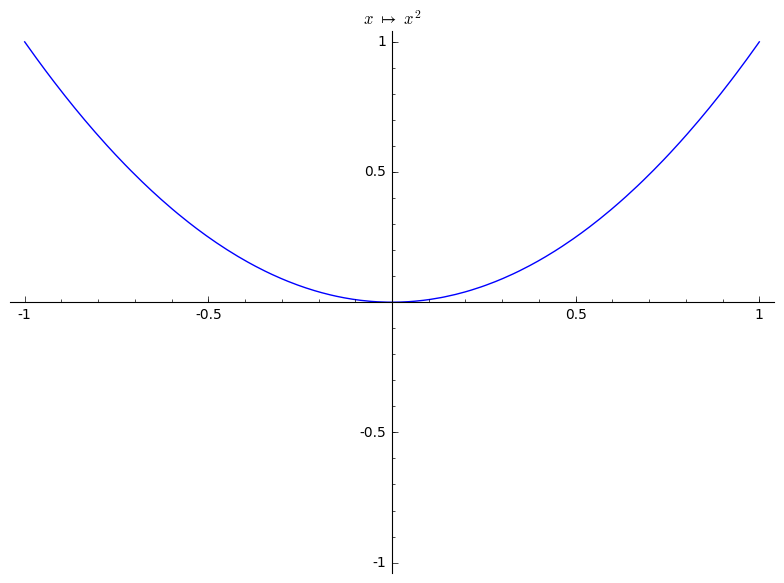
\includegraphics[width=8cm,keepaspectratio=true]{./md/IMG-04_resticcion.png}
	% IMG-04_resticcion.png: 0x0 pixel, 300dpi, 0.00x0.00 cm, bb=
	\caption{Gráfica de $x^2$}
	\label{fig:0401}
\end{figure}




\begin{proposicion}
	Si una función $f:A \to B$ es inyectiva, entonces
	$$
	f:A \to f(A)
	$$ es invertible.
\end{proposicion}



Entonces, para encontrar la inversa de $y=f(x)$, tenemos que:
\begin{enumerate}
	\item Verifique que $f(x)$ es un función $1:1.$ 
	\item Despeje la variable independiente $y$ en la ecuación $y=f(x)$ para obtener
	$$x=f^{-1}(y).$$ 
	\item Reescriba la ecuación anterior intercambiando las variables: $y=f^{-1}(x).$
\end{enumerate}







%
\subsection{Caracterización geom\'etrica}


Considera ahora una función $f:\R \to \R.$ Representemos su gráfica 
$$
\Gamma_{f}=\set{(x,y)\in\R^{2}\mid y=f(x)}
=\set{(x,f(x))}
$$
en el plano.




\begin{observacion}
	\begin{itemize}
		\item $f:\R \to \R$ es \emph{$1:1$} si cada línea \emph{horizontal} intersecta la gráfica de $f$ a lo más en un punto.
		\item $f:\R \to \R$ es \emph{sobre} si cada línea horizontal intersecta la gráfica de $f$ al menos en un punto.
		\item $f:\R \to \R$ es \emph{invertible} si cada línea horizontal intersecta la gráfica de $f$...
	\end{itemize}
	
\end{observacion}





\section*{Problemas}

\begin{problema}
	Considere las siguientes relaciones en $A=\set{1,2,3}$
	\begin{enumerate}
		\item $f=\set{(1,3),(2,3),(3,1)}$
		\item $g=\set{(1,2), (3,1)}$
		\item $h=\set{(1,3),(2,1),(1,2),(3,1)}$
	\end{enumerate}
	y determine cuales inducen funciones.
\end{problema}



\begin{problema}
	Sean $f(x)=x^{2}$ y $g(x)=x-3.$ Encuentre 
	\begin{enumerate}
		\item $f\circ g$ 
		\item $g\circ f$
	\end{enumerate}
\end{problema}




\begin{problema}
	Sean $f(x)=\sqrt{x}$ y $g(x)=\sqrt{2-x}.$ Encuentre 
	\begin{enumerate}
		\item $f\circ g$ 
		\item $g\circ f$ 
		\item $f\circ f$ 
		\item $g\circ g$
	\end{enumerate}
	
\end{problema}


 
 \begin{problema}
  Si $f:A \to B,$ y $i_{S}:S\hookrightarrow A$ es la inclusión de $S$ en $A$, entonces
  $$
  f\mid_{S}= f\circ i_{S}.
  $$
 \end{problema}
 



\begin{problema}
	Considere las siguientes funciones y sus posibles composiciones, y determine si son inyectivas, suprayectivas o biyectivas:
	
	\begin{figure}
		\centering
		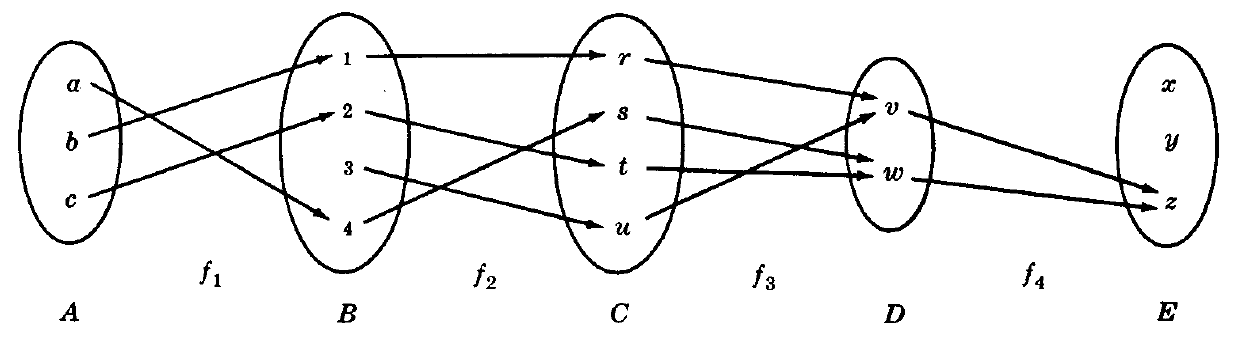
\includegraphics[width=10cm,keepaspectratio=true]{./md/MD02_IM01.png}
		% MD02_IM01.png: 0x0 pixel, 300dpi, 0.00x0.00 cm, bb=
		\label{fig:MD0201}
	\end{figure}
	
\end{problema}

\begin{figure}
	\centering
	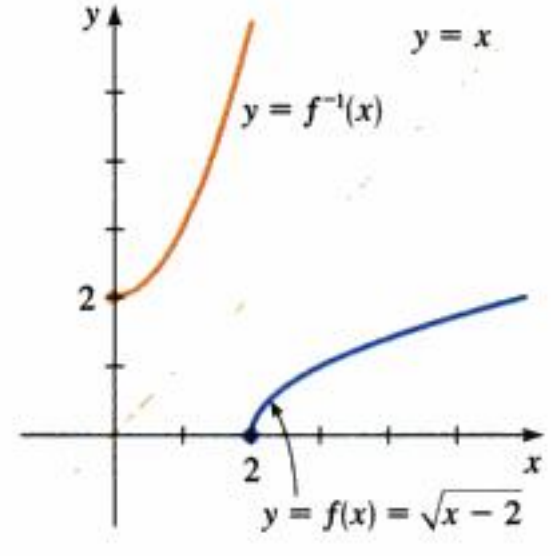
\includegraphics[height=8cm,keepaspectratio=true]{./md/MD02_sqrt_x-2.png}
	% MD02_sqrt_x-2.png: 0x0 pixel, 300dpi, 0.00x0.00 cm, bb=
	\label{fig:MD02_sqrt_x-2}
\end{figure}

\begin{figure}
	\centering
	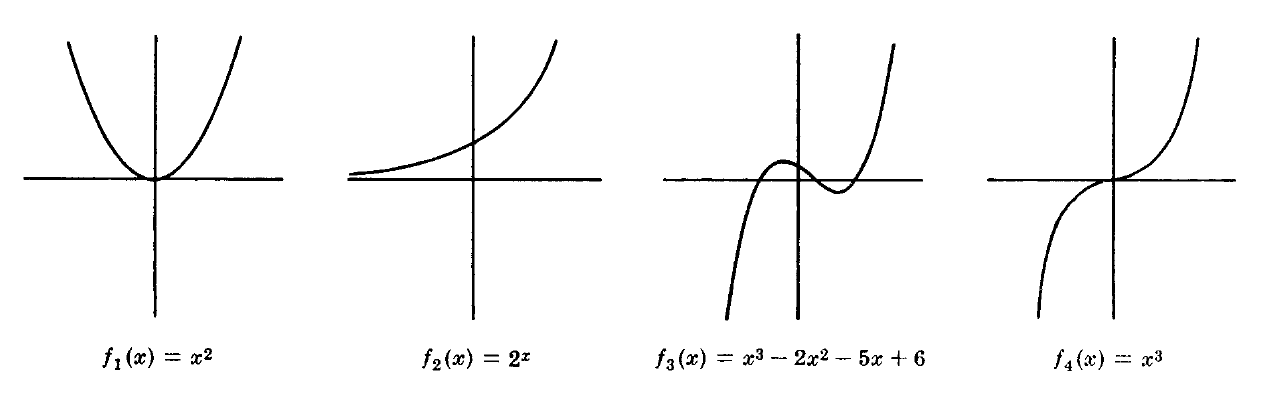
\includegraphics[width=10cm]{./md/MD02_IM02.png}
	% MD02_IM02.png: 0x0 pixel, 300dpi, 0.00x0.00 cm, bb=
	\label{fig:MD0202}
\end{figure}



\begin{problema}
	Encuentre la inversa de la función $f(x)=3x-2,$
\end{problema}




\begin{problema}
	Encuentre la inversa de $f(x)=\dfrac{x^{5}-3}{2}.$
\end{problema}




\begin{problema}
	Encuentre la inversa de $f(x)=\sqrt{x-2}.$
\end{problema}



\begin{problema}
	Considere las siguientes funciones $:\R \to \R$
	\begin{enumerate}
		\item $x \mapsto x^{2}$
		\item $x \mapsto 2^{x}$
		\item $x \mapsto x^{3}-2x^{2}-5x+6$
		\item $x \mapsto x^{3}$
	\end{enumerate}
	y determine si son $1:1,$ sobre o invertibles.
\end{problema}
\section{Particiones y conteo}



%\begin{figure}
%	\centering
%	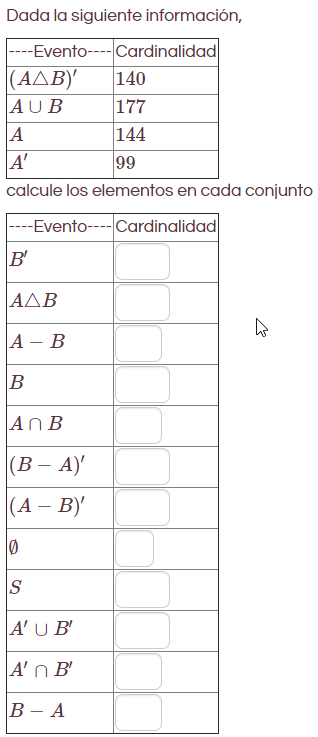
\includegraphics[height=250px]{./em/2020-08-15 19_49_02}
%	\caption{Problema de conteo}
%	\label{fig:problema-conteo}
%\end{figure}
%
%En esta actividad resolveremos el problema planteado en la figura \ref{fig:problema-conteo}. Lo abordaremos con el siguiente plan:
%\begin{enumerate}
%	\item Definir una partición en un conjunto.
%	\item Fijar una partición estándar para describir las operaciones entre dos conjuntos. 
%	\item Describir las operaciones entre conjuntos utilizando esta partición.
%	\item Plantear y resolver el problema en términos de dicha partición. 
%\end{enumerate}


\subsection{Particiones}

Consideremos un conjunto $ S $. Una partición (finita) es una colección $ \set{P_i \subset S}_{i=0}^{N}, N \in \N $ de subconjuntos de $ S $ que satisface
\begin{enumerate}
	\item $ P_i \cap P_j =\emptyset $ siempre que $ i\neq j $;
	\item $ \bigcup_{i=0}^{N} P_i = S $. 
\end{enumerate}

En otras palabras, son subconjuntos disjuntos entre sí que, al unirse todos, forman de nuevo el conjunto $ S $. El lector puede pensarlos como piezas de un rompecabezas.

\begin{figure}
	\centering
	
\includegraphics[width=0.7\linewidth]{./em/puzzle-5294291_1280}
	\caption[Rompecabezas]{Los rompecabezas son ejemplos de particiones.}
	\label{fig:puzzle-52942911280}
\end{figure}

Consideremos dos conjuntos $ A,B \subset S$. El diagrama de Ven correspondiente esta dado por la figura \ref{fig:1280px-venndiagramforaunionb}. 

\begin{figure}
	\centering
	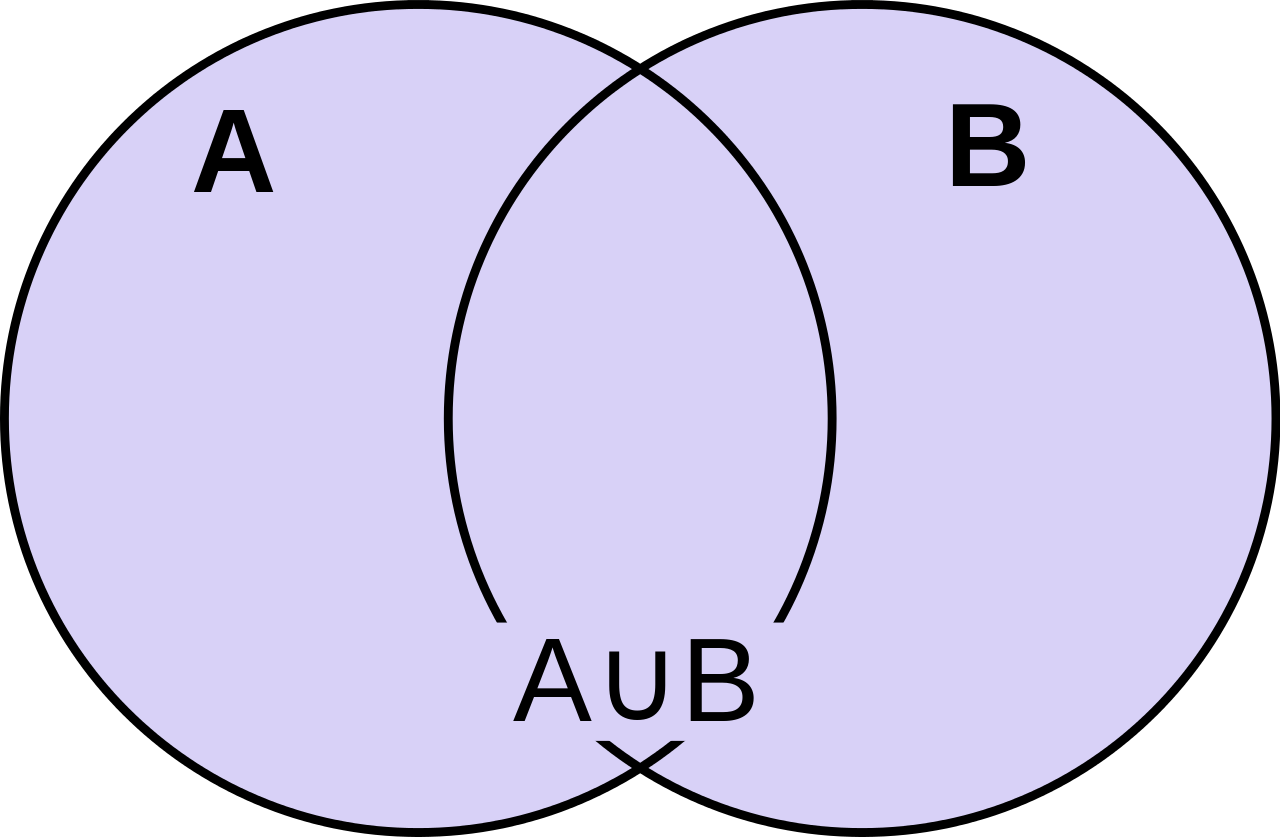
\includegraphics[width=0.7\linewidth]{./em/1280px-Venn_diagram_for_A_union_B.svg}
	\caption{Diagram de Ven para dos conjuntos}
	\label{fig:1280px-venndiagramforaunionb}
\end{figure}

Entonces podemos definir una partición $ \particion(A,B) $ para $ S $ con los siguientes elementos
\begin{itemize}
	\item $ A\cap B $
	\item $ A\backslash B = A \cap B'$
	\item $ B\backslash A = B \cap A'$
	\item $ \left(A\cup B\right)' = A'\cap B' $
\end{itemize}

Para hacer la notación más concisa, definimos las siguientes aplicaciones:
\begin{align*}
	\delta_C(x) = \begin{cases}
		1 & x \in C \\
		0 & x \not \in C
	\end{cases}
\end{align*}
donde $ 1 $ denota \texttt{verdadero}, mientras que $ 0 $ denota \texttt{falso}, y
\begin{align*}
	E_{(i,j)}=\sett{x\in S}{\delta_{A}(x)=i\wedge\delta_{B}(x)=j}
\end{align*}
De manera que 
\begin{itemize}
	\item $ A' \cap B' = E_{(0,0)}$
	\item $ A'  \cap B = E_{(0,1)}$
	\item $ A \cap B'  = E_{(1,0)}$
	\item $ A  \cap B  = E_{(1,1)}$
\end{itemize}

Para hacer aún más sencilla la notación, identificaremos la pareja $ (i,j) $ con el correspondiente número binario $ [ij]_{2} $, convertido a base 10. De manera que 
\begin{itemize}
	\item $ A' \cap B' = E_{0}$
	\item $ A'  \cap B = E_{1}$
	\item $ A \cap B'  = E_{2}$
	\item $ A  \cap B  = E_{3}$
\end{itemize}

\subsection{Planteamiento del problema}

Como los elementos de un partición son disjuntos, entonces sabemos que 
\begin{align*}
	\#\left(E_i\cup E_j\right) = \#E_i+\#E_j
\end{align*}
siempre que $ i\neq j $.

Para simplificar la notación, definimos $ x_i=\# E_i. $

La primera ecuación que se nos plantea es
\begin{align*}
	\left(A \triangle B \right)'=140,
\end{align*}
donde 
\begin{align*}
	A\triangle B = (A\backslash B)\cup(B\backslash A)
\end{align*}
es la diferencia simétrica de $ A $ con $ B $. En otras palabras $ x\in A \triangle B $ si y solo si $ x\in A $ o $ x \in B $ pero no en ambos.

Observa que entonces
\begin{align}
	\label{ec01}
	\left(A\triangle B\right)' = E_0 \cup E_3 &
	\Rightarrow
	x_0 + x_3 = 140.
\end{align}

De manera similar, obtenemos las siguientes conclusiones:
\begin{align}
	\label{ec02}
	A\cup B = E_1\cup E_2 \cup E_3 &
	\Rightarrow x_1+x_2+x_3=177 \\
	\label{ec03}
	A = E_2 \cup E_3 &
	\Rightarrow x_2+x_3 = 144 \\
	\label{ec04}
	A' = E_0 \cup E_1 &
	\Rightarrow x_0+x_1 =99
\end{align}

Al resolver el sistema de ecuaciones dado por  \ref{ec01}-\ref{ec04}, obtenemos la solución:
\begin{align*}
	x_0 &= 66 \\
	x_1 &= 33 \\
	x_2 &= 70 \\
	x_3 &= 74
\end{align*}

\subsection{Solución del problema}

A continuación presentamos el desarrollo y conclusión de cada una de las preguntas en nuestro problema. Por ejemplo, podemos describir el complemento de $ B $ en términos de nuestra partición y utilizar las soluciones anteriores. 

\begin{align*}
	\# B' 
	&= \#\left(E_1 \cup E_3\right)'\\
	&= \#\left(E_0 \cup E_2\right)\\
	&= x_0 + x_2 = 136
\end{align*}

El resto de las soluciones se encuentras de la siguiente manera:

\begin{align*}
	\card{A\triangle B} = x_1+x_2 = 103  \\
	\card{A\backslash B} = x_2 = 70 \\
	\card{B} = x_1+x_3=107	\\
	\card{A \cap B} = x_3 = 74 \\
	\card{\left(B\backslash A\right)'} 
	= x_0+x_2+x_3 = 210 \\
	\card{\left(A\backslash B\right)'}
	= x_0+x_1+x3 = 173 \\
	\card{\emptyset} = 0 \\
	\card{S} = x_0+x_1+x_2+x_3 = 243 \\
	\card{A' \cap B'} = x_0 = 66\\
	\card{B\backslash A} = x_1 = 33
\end{align*}

Con esto concluimos nuestro ejercicio. 
\section*{Problemas}

\begin{problema}
	Extiende la construcción de una partición al caso de tres subconjuntos. 
\end{problema}
\section{Análisis combinatorio}

El \emph{análisis combinatorio} es una manera sofisticada de contar.

\begin{proposicion}[Principio fundamental del conteo y diagramas de árbol]
	Si una tarea se puede realizar en $n$ formas diferentes y otra en $m$ formas diferentes, entonces las dos tareas se pueden realizar en $n\times m$ formas diferentes.	
\end{proposicion}

\begin{problema}
	\label{exmp:1.14}
\begin{enumerate}
	\item Si una persona tiene 2 camisas y 4 corbatas, ?`de cuantas formas puede combinarlas?
	\item Construya un diagrama de árbol para representar todas estas opciones.
\end{enumerate}
\end{problema}

\subsection{Permutaciones}

Consideremos un conjunto finito $X=\set{x_{1},...,x_{N}},$ esto es, $X$ tiene \emph{cardinalidad} $n(X)=N < \infty.$

Una función biyectiva (invertible) $\sigma:X \to X$ es llamada \emph{permutación} en $X.$

Observe que las composiciones e inversas de permutaciones, así como la identidad, son tambi\'en permutaciones. En este caso, diremos que la permutación $\sigma$ \emph{actua} en $X.$

Supongamos que la permutación $\sigma$ actúa en $X={x_{1},x_{2},x_{3}}$ de la siguiente manera:
$$
\sigma(x_{1})=x_{2}, \; \sigma(x_{2})=x_{3}, \; \sigma(x_{3})=x_{1}.
$$

Entonces, podemos representar la permutación de la siguiente manera
$$\sigma=
\begin{pmatrix}
	1 & 2 & 3 \\
	2 & 3 & 1,
\end{pmatrix},
$$  es decir, sólo nos fijamos de que manera actúa en el índice $j$ del elemento $x_{j}.$



De manera general, numerando los elementos de $X=\set{x_{1},...,x_{N}},$ podemos identificar este conjunto con $A_{N}=\set{1,...,N}$ por medio de la biyección $x_{i} \mapsto i.$


Ahora, consideremos una permutación $\sigma:A_{N}\to A_{N},$ tal que $\sigma(i)=\sigma_{i}.$ Entonces podemos representa $\sigma$ por medio de 
$$\sigma=
\begin{pmatrix}
	1& ... & N \\
	\sigma_{1}& ... & \sigma_{N}.
\end{pmatrix}
$$


El conjunto de todas las permutaciones $:A_{N}\to A_{N}$ se denota por $S_{N}$ y tiene una cardinalidad 
$n(S_{N})=N!.$

\subsection{Cálculos con permutaciones}
Si tenemos $n$ objetos distintos y queremos ordenarlos tendremos
\begin{align*}
	n \times (n-1) \times ... 2\times 1
\end{align*} formas diferentes de hacerlo.

{}
\begin{definicion}[$n$ factorial]
	\[
		n! = \begin{cases}
			1 & n=0 \\
			n\times(n-1)! & n>0
		\end{cases}
	\]
	
\end{definicion}


Si tenemos $n$ objetos distintos y queremos arreglar $r$ de estos en una linea, entonces tendremos una \emph{permutación} de $n$ en $r$ dada por
\begin{align}
	\label{1.25}
	P^{n}_{r}=n\times(n-1)\times...\left( n-r+1 \right)
\end{align} 
o de manera equivalente
\begin{align}
	\label{1.27}
	P^{n}_{r}=\dfrac{n!}{(n-r)!}
\end{align}



\subsection{Combinaciones}
{}
En una \emph{permutación}, uno está interesado en el orden de los objetos. Así $abc$ y $bca$ son permutaciones diferentes.  Pero en algunos problemas, uno está interesado sólo en elegir objetos sin importar su orden.  Tales selecciones se llaman \emph{combinaciones}.  Por ejemplo, $abc$ y $bca$ representan la misma combinación.



El número de combinación $ C^{n}_{r} $ al elegir $r$ objetos de una colección de $n$ diferentes está dada por el \emph{número combinatorio}
\begin{align}
	\label{1.29}
	C^{n}_{r} = \comb{n}{r}=\dfrac{n!}{r!\left( n-r \right)!}
\end{align}



{Algunas fórmulas combinatorias}
\begin{align}
	\label{1.30}
	\comb{n}{r}&=\dfrac{P(n,r)}{r!} \\
	\label{1.31}
	\comb{n}{r}&=\comb{n}{n-r}\\
	\comb{n}{r}&=\comb{n-1}{r-1}+\comb{n-1}{r}
\end{align}


\subsection{El Teorema del Binomio}

\begin{teorema}[Teorema del binomio]
	\begin{align}
		\label{1.32}
		\left( x+y \right)^{n} = \sum_{r=0}^{n}\comb{n}{r}x^{r}y^{n-r}
	\end{align}
	
\end{teorema}

%\begin{proposicion}[Aproximación de Stirling]
%	\begin{align*}
%		\label{1.33}
%		n! \approx \sqrt{2\pi n}\left( n^{n}e^{-n} \right)
%	\end{align*}
%\end{proposicion}





\section*{Problemas}
{}
\begin{problema}
	\label{solved:1.22}
	Se requiere sentar a $5$ hombres y $4$ mujeres en una fila, de manera que estén alternados. ?`Cuantas manera hay de hacer tal arreglo?
\end{problema}


{}
\begin{problema}
	\label{exmp:1.16}
	?`Cuantas permutaciones de longitud 3 se pueden formar con las letras $A,B,C,D,E,F,G$?
\end{problema}


{}
\begin{problema}
	\label{exmp:1.17}
	Encuentre el número de permutaciones diferentes de las 11 letras de la palabra \emph{MISSISSIPPI}.
\end{problema}

\begin{problema}
	\label{solved:1.29}
	?`De cuantas manera podemos formar un equipo de 11 personas de un total de 23?
\end{problema}

{}
\begin{problema}
	\label{solved:1.35}
	Una caja contiene $8$ canicas rojas, $3$ blancas y $9$ azules. Si 3 canicas son obtenidas al azar sin reemplazarse, determine la probabilidad de que
	\begin{enumerate}
		\item las tres sean rojas; 
		\item las tres sean blancas; 
		\item dos sean rojas y una blanca; 
		\item al menos una sea blanca; 
		\item una sea de cada color; 
		\item sean obtenidas en el siguiente orden: rojo, blanco y azul.
	\end{enumerate}
	
\end{problema}

{}
\begin{problema}
	\label{solved:1.36}
	En un juego de \emph{poker}, 5 cartas se obtienen al azar de una baraja inglesa. Encuentre la probabilidad de que
	\begin{enumerate}
		\item 4 sean $A$; 
		\item 4 sean $A$ y una sea $K$; 
		\item 3 sean $10$ y dos sean $J$; 
		\item $9,10,J,Q,K$ en cualquier order; 
		\item 3 de un palo dado y 2 de otro palo; 
		\item al menos un $A$ obtenido.
	\end{enumerate}
	
\end{problema}

{}
\begin{problema}
	\label{solved:1.37}
	Determine la probabilidad de obtener tres $6$ en cinco lanzamientos de un dado.
\end{problema}

\begin{problema}
	\label{exmp:1.18}
	En una baraja inglesa, ?`cuantas formas hay de escoger dos cartas del mismo palo?
\end{problema}


\chapter{Aritmética}

%101
\section{Los números enteros}
	
	En esta sección analizaremos algunos conjuntos numéricos. 
	Los números naturales son el conjunto de números
	$$
	\N=\set{0,1,2,3,...},
	$$	
	mientras que los números enteros son el conjunto de números
	$$
	\Z=\set{0, \pm1, \pm2,...}	$$	


\subsection{Máximo Común Divisor}
	
\begin{definicion}
	Diremos que un entero $n$ divide a otro entero $c\in \Z$ si existe un tercer entero $p\in \Z$ tal que 
	$$c=n\cdot p.$$
\end{definicion}

\begin{definicion}
	\label{mcd} 
	Diremos que el entero $d$ es el \emph{máximo común divisor} de dos enteros $a,b$ o $\texttt{mcd}(a,b)$  si
	\begin{itemize}
		\item $d$ divide tanto a $a$ como $b$ y;
		\item $d$ es el número entero más grande con esta propiedad.
	\end{itemize}
\end{definicion}

	\begin{problema}
		\label{exmp:mcd}
		Encontremos $\texttt{mcd}(6,15).$ Los divisores de $6$ son $\pm1, \pm2, \pm3, \pm6,$ mientras que los de $15$ son $\pm1, \pm3, \pm5, \pm15.$
		
		Entonces, los divisores en común de $6$ y $15$ son $\pm1,\pm3.$ El más grande de todos estos es 
		$d=3$ y por tanto es $$ \texttt{mcd}(6,15)=3. $$
	\end{problema}
	
 	Aunque este m\'etodo para encontrar el \texttt{mcd} es útil cuando hay pocos divisores, puede resultar abrumador si  	ambos números tienes una gran cantidad de divisores. 
   
	\begin{proposicion}[Teorema del Residuo]
		\sidenote{
			Consulta \citep[sección 7.2, teorema 1]{cardenas1973algebra} para ver una demostración.
		}
		Dados dos números enteros positivos $a,b,$ existen otro par de enteros $q, r\geq 0$ tales que
		\begin{align}
			\label{cociente}
			a=b\cdot q+r\\
			\label{residuo}
			r<b.
		\end{align}
		A $q$ se le llama cociente, mientras que a $r$ se le llama residuo.
	\end{proposicion}




	\begin{problema}
		Si $a=7,b=2$, entonces el cociente es $q=3$ y el residuo es $r=1,$ porque
		$$\begin{cases}
			7=2\cdot 3+1\\ {r=1}<{b=2}.     
		\end{cases}
		$$
	\end{problema}

		Observe que tambien podr\'iamos tomar $q=1, r=5$ y escribir $$7=2\cdot 1+5,$$ pero como ${5}>{2},$ entonces $r=5$ no 
		satisface la condici\'on del residuo \eqref{residuo}, porque ${r=5}\geq {b=2}.$

	\begin{algoritmo}{Algoritmo Euclidiano}
		\sidenote{	
	Consulta \citep[sección 7.4, prop. 1]{cardenas1973algebra} para ver una demostración.	
	}
		Sean $a,b\in \Z$ dos números enteros positivos. Consideremos la siguiente sucesi\'on de operaciones, en la que iteramos el teorema del residuo:
		\begin{align*}
			a&=b\cdot q_{0}+r_{0} \\
			b&=r_{0}\cdot q_{1}+r_{1}\\
			r_{0}&=r_{1}\cdot q_{2}+r_{2}\\
			&...\\
			r_{N-3}&=r_{n-2}\cdot q_{N-1}+r_{N-1}\\
			r_{N-2}&=r_{N-1}\cdot q_{N}+0.
		\end{align*}
		Entonces el último cociente $r_{N-1}$ es el \texttt{mcd} de $a$ y $b.$
	\end{algoritmo}
	
	
	Como en el ejemplo \ref{exmp:mcd}, tenemos que 
	\begin{align*}
		15&=6\cdot 2+3\\ 
		6&=3\cdot 2+0, 
	\end{align*}
	Entonces $r=3$ es igual a $\texttt{mcd}(15,6)$.



\subsection{M\'inimo Común Múltiplo}


	\begin{definicion}
		\label{mcm} 
		Diremos que el entero positivo $m\in \Z$ es el \emph{m\'inimo común multiplo} o $\texttt{mcm}$ de dos enteros positivos $a,b$ si
		\begin{itemize}
			\item $m$ es múltiplo tanto de de $a\in \Z$ como $b\in \Z$ y;
			\item $d$ es el número entero positivo más pequeño con esta propiedad.
		\end{itemize}		
	\end{definicion}
	
	\begin{proposicion}
		\sidenote{	
	Consulta \citep[sección 7.5, ejercicios del 10 al 12]{cardenas1973algebra} para ver una demostración.	
	}
		\label{prop:mcm}
		Si $a,b$ son dos enteros positivos, entonces
		$$
		\texttt{mcm}(a,b)\texttt{mcd}(a,b)= a\cdot b
		$$
	\end{proposicion}

	\begin{problema}
		\label{exmp:mcm}
		Encontremos el $\texttt{mcm}$ de $a=6$ y $b=15.$
		Como vimos anteriormente, $ \mcd(6,15)=3 $. Entonces, 
		\[ \mcm(6,15)=\dfrac{6\cdot15}{3}= 30 \].
	\end{problema}



\input{numeros_enteros(p)}
\section{Teorema Fundamental de la Aritmética}

%%%%%%%%%%%%%%%%%%%%%
{}
Un número primo $p$ es aquel que tiene exactamente cuatro divisores
\begin{align*}
\pm 1, \pm p.
\end{align*}


%%%%%%%%%%%%%%%%%%%%%
{}
\begin{problema}
Encuentre los números primos (positivos) entre 2 y 100.
\end{problema}


%%%%%%%%%%%%%%%%%%%%%
{}
Los números enteros siempre se pueden escribir como una multiplicación de números primos:
\begin{itemize}
\item $36=2^{2}3^{2}$
\item $1400=2^{3}5^{2}7$
\item $187=11\times 7$
\end{itemize}


%%%%%%%%%%%%%%%%%%%%%
{Teorema Fundamental de la Aritmética}
\begin{teorema}
	Todo número entero $a$ mayor que $1$ se puede expresar en la forma
	\begin{align*}
		\label{factorizacion_prima}
		\tag{FP}
		a=p_{1}^{n_{1}}p_{2}^{n_{2}}\cdots p_{L}^{n_{L}}
	\end{align*}
	donde $p_{i}, i=1,...,L$ son números primos distintos y $n_{i}, i=1,...,L$ son exponentes enteros positivos. 
\end{teorema}

\begin{observacion}
	La expresión \ref{factorizacion_prima} se conoce como \emph{factorización prima} del entero $a$ y es única excepto por el orden.
\end{observacion}

%%%%%%%%%%%%%%%%%%%%%
{}
Encuentre la factorización prima de 
\begin{itemize}
\item $14700 = 2^{2}\cdot 3 \cdot 5^{2} \cdot 7^{2}$
\item $1575 = 3^{2}\cdot 5^{2} \cdot 7$
\end{itemize}


%%%%%%%%%%%%%%%%%%%%%
{}
\begin{proposicion}
	Si $a=p_{1}^{n_{1}}p_{2}^{n_{2}}\cdots p_{L}^{n_{L}}$ y $b=p_{1}^{m_{1}}p_{2}^{m_{2}}\cdots p_{L}^{m_{L}}$ son respectivas factorizaciones primas de los enteros $a,b$, entonces
	\begin{align*}
		\mcd(a,b) &= p_{1}^{r_{1}}p_{2}^{r_{2}}\cdots p_{L}^{r_{L}}\\
		\mcm(a,b) &= p_{1}^{R_{1}}p_{2}^{R_{2}}\cdots p_{L}^{R_{L}}
\end{align*}
donde $r_{i}=\min(n_{i},m_{i})$ y $R_{i}=\max(n_{i},m_{i}).$
\end{proposicion}


%%%%%%%%%%%%%%%%%%%%%
{}
Encuentre
\begin{itemize}
	\item $\mcd(14700,1575) = 3 \cdot 5^{2} \cdot 7=525$ 
	\item $\mcm(14700,1575) = 2^{2} \cdot 3^{2} \cdot 5^{2} \cdot 7^{2}= 44100$
\end{itemize}


%%%%%%%%%%%%%%%%%%%%%
{}
	\begin{proposicion}
		Si $p_{1}^{n_{1}}p_{2}^{n_{2}}\cdots p_{L}^{n_{L}}$ es la factorización prima de $a$, entonces $a$ tiene \begin{align*}
			\left( n_{1}+1 \right)\left( n_{2}+1 \right)\cdots\left( n_{L}+1 \right)
		\end{align*} divisores positivos.
		
	\end{proposicion}
	

%%%%%%%%%%%%%%%%%%%%%% 


	\begin{algoritmo}{Como encontrar todos los divisores de un número entero}
		\begin{enumerate}
			\item Factorice el número entero
			$n=p_{1}^{R_{1}}\cdots p_{m}^{R_{m}}$
			\item Enliste cada posible $m-$tupla
			$\left( r_{1},...,r^{m} \right)$
			con $0\leq r_{1}\leq R_{1},...,0\leq r_{m}\leq R_{m}$
			\item Enliste cada posible número entero de la forma $$\pm p_{1}^{r_{1}}\cdots p_{m}^{r_{m}},$$ para cada elemento $\left( r_{1},...,r_{m} \right)$ de la lista anterior.
		\end{enumerate}
	\end{algoritmo}
	


%%%%%%%%%%%%%%%%%%%%%

{Cálculo de divisores}
	\begin{problema}
		Encuentre todos los divisores positivos de $24$.
	\end{problema}
	
	Los divisores son 1, 2, 3, 4, 6, 8, 12, y 24.
	

%%%%%%%%%%%%%%%%%%%%%
{}
	\begin{problema}
		Encuentre todos los divisores positivos de $72$.
	\end{problema}
	
	Los divisores son 1, 2, 3, 4, 6, 8, 9, 12, 18, 24, 36, y 72
	

%%%%%%%%%%%%%%%%%%%%%
{}
	\begin{problema}
		Encuentre todos los divisores positivos de $600$.
	\end{problema}
	
	Los divisores son 1, 2, 3, 4, 5, 6, 8, 10, 12, 15, 20, 24, 25, 30, 40, 50, 60, 75, 100, 120, 150, 200, 300, y 600.



\section{Inducción Matemática}

\subsection{Introducción}


	Una propiedad esencial de los naturales $\N=\set{1,2,3,...}$  es la siguiente
	
	
	\begin{ax}[Principio de Inducción Matemática, versión I]
		Sea $P$ una proposición definida en $\N,$ es decir, $P(n)$ toma valores de cierto o falso para cada $n\in \N.$
		
		Supongamos que
		\begin{enumerate}
			\item $P(1)$ es cierto;
			\item $\forall k \in \N: P(k) \onlyif P(k+1).$
		\end{enumerate}
		
		Entonces $P$ es {cierto} para todo entero positivo $n\in \N.$
	\end{ax}
	



	\begin{problema}
		Sea $P(n):1+3+5+...+(2n-1)=n^2.$ Demostrar que $P(n)$ es cierta para toda $n \in \N.$ 
	\end{problema}



	\begin{ax}[Principio de Inducción Matemática, versión II]
		Sea $P$ una proposición definida en $\N$ tal que :
		\begin{enumerate}
			\item $P(1)$ es cierta;
			\item $P(k)$ es cierta siempre que $P(j)$ para toda $1\leq j < k.$
		\end{enumerate}
		Entonces $P(n)$ es cierta para toda $n\in \N.$
	\end{ax}
	



	\begin{observacion}
		Algunas veces, uno desea demostrar que una proposición es cierta para algún conjunto de enteros
		$$
		\set{a,a+1, a+2,...}
		$$
		donde $a$ es un entero positivo, posiblemente cero. Esto puede hacerse simplemente reemplazando $1$ por $a$ en cualquier versión del Principio de Inducción Matemática. 
	\end{observacion}
	
	\begin{problema}
	Demostrar que $$P(n): 1+2+3+...+n=\frac{1}{2}n\left( n+1 \right)$$
	es cierto para todo $n \in \N.$
\end{problema}




\begin{problema}
	Demostrar que $$P(n): 1+2+2^{2}+...+2^{n}=2^{n+1}-1$$
	es cierto para todo $n \in \N.$
\end{problema}

\subsection{Notación ``Sigma''}


	La letra griega $\Sigma$ denota adición repetida:
	
	$$
	\sum_{i=a}^{b} f(i)=f(a)+f(a+1)+...+f(b),
	$$ siempre que $a\leq b.$



	\begin{problema}
		\label{ayr:exmp23.1}
		\begin{enumerate}
			\item $\sum_{j=1}^{5} j = 1+2+3+4+5 =15$
			\item $\sum_{i=0}^{3} \left( 2i+1 \right)=
			1+3+5+7$
			\item $\sum_{i=2}^{10} i^{2}=2^{2}+3^{2}+...+10^{2}$
			\item $\sum_{j=1}^{4}\cos(j\pi)=
			\cos\pi+ \cos 2\pi + \cos 3\pi +\cos 4\pi.$
		\end{enumerate}
		
	\end{problema}
	



	{Linealidad}
	\begin{proposicion}
		\label{suma:linealidad}
		\begin{align*}
			\sum_{i=a}^{b} cf(i)&=c \sum_{i=a}^{b} f(i)\\
			\sum_{i=a}^{b} f(i)+g(i)&= \sum_{i=a}^{b} f(i)
			+\sum_{i=a}^{b} g(i)
		\end{align*}
		
	\end{proposicion}
	



	{Propiedades}
	\begin{align*}
		\sum_{k=a}^{b}f(k)&=\sum_{j=a}^{b}f(j)\\
		\sum_{j=a}^{a}f(j)&=f(a) \\
		\sum_{j=a}^{c}f(j)&=\sum_{j=a}^{b}f(j)+\sum_{j=b}^{c}f(j) \\
		\sum_{j=a}^{b+1}f(j)&=\sum_{j=a}^{b}f(j)+f(b)
	\end{align*}
	



	\begin{problema}
		Si $f(n)=(2n-1),$ entonces
		$$
		\sum_{i=1}^{n}f(j)=1+3+...+\left( 2n-1 \right)
		$$ es la suma hasta el $n-$\'esimo natural impar.  Observe que 
		\begin{enumerate}
			\item $\sum_{j=1}^{1}f(j)=2(1)-1=1.$
			\item $\sum_{i=1}^{n+1}f(j)=\left( \sum_{i=1}^{n}f(j) \right)+\left( 2n+1 \right)$
		\end{enumerate}
		
	\end{problema}
	



	\begin{problema}
		Si $f(n)=2^{n-1},$ entonces
		$$
		\sum_{i=1}^{n}f(j)=1+2+...+2^{n-1}
		$$ es la suma de las primeras $n$ potencias de 2 (incluyendo $1=2^{0}$).  Observe que 
		\begin{enumerate}
			\item $\sum_{i=1}^{n+1}f(j)=1+2+...+2^{n}$
			\item $\sum_{j=1}^{1}f(j)=2^{1-1}=1.$
			\item $\sum_{i=1}^{n+1}f(j)=\left( \sum_{i=1}^{n}f(j) \right)+2^{n}.$
		\end{enumerate}
		
	\end{problema}
	


\subsection{Ejemplos Resueltos}


	\begin{problema}
		Demostrar que $$P(n): 1+2+3+...+n=\frac{1}{2}n\left( n+1 \right)$$
		es cierto para todo $n \in \N.$
	\end{problema}
	



	\begin{problema}
		Demostrar que $$P(n): 1+2+2^{2}+...+2^{n}=2^{n+1}-1$$
		es cierto para todo $n \in \N.$
	\end{problema}
	


\subsection{Funciones definidas de manera recursiva}


	Decimos que una función está \emph{definida recursivamente} si la definición de la función se refiere a sí misma.



	Para que la función est\'e bien definida, debe tener las siguientes dos propiedades:
	\begin{enumerate}
		\item Deben existir ciertos argumentos, llamados \emph{valores base,} para los cuales la función no se refiera a sí misma.
		\item Cada vez que la función se refiera a sí misma, el argumento de la función debe estár más cercano a un valor base.
	\end{enumerate}
	


\subsection{La función factorial}


	El producto de enteros positivos de $1$ hasta $n$ (incluído) es llamado \emph{$n$ factorial, $n!$}
	
	Es decir, 
	$$
	n!=n(n-1)\cdots 3\cdot 2 \cdot 1.$$
	



	Por razones combinatorias, es conveniente definir \emph{$0!=1,$} y de esta manera la función factorial quedará definida para todos los enteros no negativos.



	\begin{observacion}
		\begin{enumerate}
			\item $1!=1\cdot0!$
			\item $2!=2\cdot1!$
			\item $3!=3\cdot2!$
			\item $4!=4\cdot3!$
		\end{enumerate}
		
	\end{observacion}
	



	Es fácil observar que para $n \in \N:$
	$$
	n!=n\cdot (n-1)!
	$$



	\begin{definicion}[Función factorial]
		$$n!=
		\begin{cases}
			1 & n=0 \\
			n\cdot(n-1)! & n>0
		\end{cases}
		$$
	\end{definicion}
	



	\begin{observacion}
		\begin{enumerate}
			\item El valor de $n!$ factorial esta dado explicitamente para $n=0,$ de manera que $0$ es el valor base. 
			\item El valor de $n!, n>0$ está dado en t\'erminos de $n-1,$ que es más cercano al valor base $0.$    
		\end{enumerate}
		
		Por tanto, $n!$ es una función recursiva bien definida.
	\end{observacion}
	


\begin{lstlisting}[language=python, caption=Implementación iterativa del \emph{factorial} en \texttt{Python}]
def factorial(n):
	result = 1
	for i in range(1, n+1):
		result *= i
	return result
\end{lstlisting}

\begin{lstlisting}[language=python, caption=Implementación recursiva del \emph{factorial} en \texttt{Python}]
def factorial(n):
	z=1
	if n>1:
		z=n*factorial(n-1)
	return z
\end{lstlisting}

Para más implementaciones, visite \href{https://rosettacode.org/wiki/Factorial}{Rosetta Code.}



\subsection{Suceción de Fibonacci}


	La celebre sucesión de Fibonacci (usualmente denotada por $F_{0}, F_{1}, F_{2},...$) es como sigue:
	$$
	0,0,1,2,3,5,8,13,21,34,55,...
	$$
	
	Es decir, $F_{0}=0$  $F_{1}=1$ y cada t\'ermino sucesor es la suma de los dos precedentes.



	Por ejemplo, los siguientes dos t\'erminos de la sucesión son
	$$34+55=89 \texttt{ y }55+89=144.$$



	\begin{definicion}[Sucesión de Fibonacci]
		$$
		F_{n}=
		\begin{cases}
			n & n=0,1 \\
			F_{n}=F_{n-2}+F_{n-1} & n>1
		\end{cases}
		$$
	\end{definicion}



	Este ejemplo es una función recursiva bien definida, ya que la función hace referencia a sí misma, cuando se usan $ F_{n-2}$ y $F_{n-1},$ y
	\begin{enumerate}
		\item los valores base son $0$ y $1;$
		\item los valores de $F_{n}$ están definidos en t\'erminos de valores más peque\~nos $n-2$ y $n-1$ que son más cercanos a los valores base.
	\end{enumerate}
	


\begin{lstlisting}[language=Python, caption=Implentación iterativa de \emph{Fibonacci} en \texttt{Python}]		
def fibIter(n):
	if n < 2:
		return n
	fibPrev = 1
	fib = 1
	for num in xrange(2, n):
		fibPrev, fib = fib, fib + fibPrev
	return fib
\end{lstlisting}
	
%\begin{lstlisting}
%def fibIter(n):
%	if n < 2:
%		return n
%	fibPrev = 1
%	fib = 1
%	for num in xrange(2, n):
%		fibPrev, fib = fib, fib + fibPrev
%	return fib
%\end{lstlisting}

\begin{lstlisting}[language=Python, caption=Implentación recursiva de \emph{Fibonacci} en \texttt{Python}]
def fibRec(n):
	if n < 2:
		return n
	else:
		return fibRec(n-1) + fibRec(n-2)
\end{lstlisting}

Para más implementaciones, visita \href{http://rosettacode.org/wiki/Fibonacci\_sequence}{Rosetta Code.}


\subsection{La función de Ackermann}


	\begin{definicion}[Función (fallida) de Ackermann]
		$$
		A(m,n)=
		\begin{cases}
			n+1 & m=0\\
			A(m-1,n) & m\neq0, n=0 \\
			A(m-1, A(m,n-1)) & m\neq 0, n\neq 0
		\end{cases}
		$$
	\end{definicion}
	



	\begin{definicion}[Función de Ackermann]
		$$
		A(m,n)=
		\begin{cases}
			n+1 & m=0\\
			A(m-1,1) & m\neq0, n=0 \\
			A(m-1, A(m,n-1)) & m\neq 0, n\neq 0
		\end{cases}
		$$
	\end{definicion}
	


\begin{lstlisting}[caption=python, caption=Implentación recursiva de \emph{Ackermann} en \texttt{Python}]
def ack2(M, N):
	if M == 0:
		return N + 1
	elif N == 0:
		return ack2(M - 1, 1)
	else:
		return ack2(M - 1, ack2(M, N - 1))
\end{lstlisting}

Para más implementaciones, visite \href{http://rosettacode.org/wiki/Ackermann\_function}{Rosetta Code.}



\section*{Problemas}


\begin{problema}
	Sean $a,b$ enteros positivos, y definamos la siguiente función de manera recursiva:
	$$
	Q(a,b)=
	\begin{cases}
		0 & a<b \\
		Q(a-b,b)+1 & b \leq a
	\end{cases}
	$$
	\begin{enumerate}
		\item Encuentre (i) $Q(2,5);$ (ii) $Q(12,5)$
		\item ?`Qu\'e es lo que hace esta función? Encuentre $Q(5861,7)$
	\end{enumerate}
\end{problema}



\begin{problema}
	Use la definición de la función de Ackermann para calcular $A(1,3).$
\end{problema}



\begin{problema}
	Demuestre por inducción que 
	$\displaystyle 2+4+6+...+2n=n(n+1)$
\end{problema}



\begin{problema}
	Demuestre por inducción que 
	$\displaystyle 1+4+7+...+\left( 3n-2 \right)=\dfrac{n\left( 3n-1 \right)}{2}$
\end{problema}



\begin{problema}
	Demuestre por inducción que 
	$\displaystyle 1^{2}+2^{2}+...+n^{2}=\dfrac{n(n+1)(2n+1)}{6}$
\end{problema}



\begin{problema}
	Demuestre por inducción que 
	$\displaystyle \dfrac{1}{1\cdot 3}+\dfrac{1}{3\cdot 5}+...+\dfrac{1}{\left( 2n-1 \right)\cdot \left( 2n+1 \right)}=\dfrac{n}{2n+1}$
\end{problema}



\begin{problema}
	Demuestre por inducción que 		
	$\displaystyle \dfrac{1}{1\cdot 5}+ \dfrac{1}{5 \cdot 9}+...+\dfrac{1}{(4n-3)\cdot (4n+1)}=\dfrac{n}{4n+1}$
\end{problema}



\begin{problema}
	Demuestre por inducción que 		
	$7^{n}-2^{n}$ es divisible entre $5$
\end{problema}



\begin{problema}
	Demuestre por inducción que 		
	$n^{3}-4n+6$ es divisible entre $3$
\end{problema}



\begin{problema}
	La función de Ackermann está definida de manera recursiva de las siguiente manera:
	$$
	A(m,n)=
	\begin{cases}
		n+1 & m=0\\
		A(m-1,1) & m\neq0, n=0 \\
		A(m-1, A(m,n-1)) & m\neq 0, n\neq 0
	\end{cases}
	$$
	Encuentre $A(1,1)$.		
\end{problema}



\chapter{Sistemas numéricos}

%102
\section{Los números racionales}


	Los números racionales son el conjunto de números
	$$
	\Q=\set{\frac{a}{b} \mid a,b \in \Z, b\neq 0} 
	$$
identificando $\dfrac{a}{b}=\dfrac{c}{d}$ siempre que la \emph{razón cruzada} sea igual
\begin{align*}
ad=bc
\end{align*}


%%%%%%%%%%%%%%%%%%%%%


	¿Para que nos sirve $\Q$? 
	
	Este conjunto de números nos sirve para \emph{contar, sumar, restar, multiplicar y dividir.}



	\begin{definicion}
		\label{rat:equiv}
		Dos números racionales $\dfrac{a}{b},\dfrac{c}{d}$ son equivalentes si
		$$
		ad-bc=0.
		$$
	\end{definicion}

%%%%%%%%%%%%%%%%%%%%%
{}

	\begin{problema}
		$\dfrac{1}{2}$ es equivalente a $\dfrac{2}{4}$ porque
		$$
		\left( 1 \right)\left( 4 \right)-\left( 2 \right)\left( 2 \right)=0.
		$$
	\end{problema}
	


\subsection{Simplificaci\'on}

 
	\begin{definicion}
		\begin{enumerate}
			\item Diremos que dos enteros $p,q\in \Z$ son primos relativos si $\texttt{mcd}(p,q)=1.$ 
			\item Diremos que $\dfrac{p}{q}\in \Q$ es la forma \emph{irreducible} de $\dfrac{a}{b}\in \Q$ si 
			\begin{itemize}
				\item $\dfrac{p}{q}$ es equivalente a $\dfrac{a}{b}$ y
				\item $p,q$ son primos relativos.
			\end{itemize}
			
		\end{enumerate}
		
	\end{definicion}
	




	Por la definici\'on \ref{rat:equiv}, tenemos que para un número racional $\frac{a}{b}:$
	$$
	\dfrac{n\cdot a}{n\cdot b}=\dfrac{a}{b},
	$$
	siempre que $n\neq 0.$
	
	\begin{problema}
		$\dfrac{2}{4}=\dfrac{2*1}{2*2}=\dfrac{1}{2}.$
	\end{problema}
	

% 
% 
%  \begin{definicion}
%   Diremos que la forma irreducible de una fracci\'on $\dfrac{a}{b}$ es $\dfrac{p}{q}$ si
%   \begin{itemize}
%    \item $$\dfrac{a}{b}=\dfrac{p}{q},$$ pero
%    \item $p,q$ son primos relativos.
%   \end{itemize}
% 
%  \end{definicion}
% 
% 


	\begin{observacion}
		Sean $a,b$ dos enteros positivos.
		Si $d=\texttt{mcd}(a,b)$ y $$a=d\cdot p, \, b=d\cdot q,$$ entonces podemos simplificar de la siguiente manera
		$$
		\dfrac{a}{b}=\dfrac{d\cdot p}{d \cdot q}=\dfrac{p}{q}.
		$$
	\end{observacion}




	\begin{observacion}
		Si $d$ es el máximo común divisor de los enteros $a,b\neq 0,$ entonces tenemos que $p,q$ son los cocientes en las operaciones
		$$\begin{cases}
			a=d\cdot p \\
			b=d\cdot q
		\end{cases}
		$$
	\end{observacion}
	



	\begin{problema}
		Encuentre la forma irreducible de $\dfrac{15}{10}.$
	\end{problema}



	
	\begin{solucion}
		\begin{enumerate}
			\item Primero, muestre que $\texttt{mcd}(15,10)=5;$ 
			\item Como $$\dfrac{15}{10}=\dfrac{5\cdot 3}{5\cdot 2}=\dfrac{3}{2},$$ entonces $\dfrac{3}{2}$ es equivalente a 
			$\dfrac{15}{10}$ 
			\item Finalmente muestre que $3$ y $2$ son primos relativos. Concluimos que $\dfrac{3}{2}$ es la forma irreducible de 
			$\dfrac{15}{10}.$ 
		\end{enumerate}
		
	\end{solucion}



	\begin{problema}
		Encuentre la forma irreducible de la fracci\'on $$\dfrac{182}{910}$$
	\end{problema}
	



\subsection{Conversi\'on y comparaci\'on}


	Supongamos que una pizza se parte en 12 rebanadas iguales, mientras que otra similar se parte en 8. ¿Qu\'e cantidad de pizza es mayor, 7 rebanadas de la primera o 5 de la segunda?



	Para comparar dos fracciones, debemos convertirlas de manera que tenga un común denominador. 



	\begin{algoritmo}{Conversi\'on a común denominador}
		Para convertir dos fracciones $\frac{a}{b}, \frac{c}{d}$ a común denominador:
		\begin{enumerate}
			\item Encuentre $m=\texttt{mcm}(b,d)$
			\item Encuentre un entero $p$ tal que $m=b\cdot p$ y convierta la primera fracci\'on
			$$
			\dfrac{a}{b}=\dfrac{a\cdot p}{b \cdot p}=\dfrac{ap}{m}
			$$
			\item Encuentre un entero $q$ tal que $m=d\cdot q$ y convierta la segunda fracci\'on
			$$
			\dfrac{c}{d}=\dfrac{c\cdot q}{d \cdot q}=\dfrac{cq}{m}
			$$
		\end{enumerate}
		
	\end{algoritmo}
	



	\begin{observacion}
		Si el común demoninador $m$ de dos fracciones $$\dfrac{x}{m}, \dfrac{y}{m}$$ es positivo, entonces
		$$
		\dfrac{x}{m} < \frac{y}{m} \iff x < y.
		$$
	\end{observacion}
	




	\begin{problema}
		Compare cada uno de los siguientes pares de fracciones:
		\begin{enumerate}
			\item $\dfrac{15}{11}, \dfrac{28}{37}$ 
			\item $-\dfrac{35}{36}, \dfrac{1}{6}$
			\item $\dfrac{3}{10}, -\dfrac{23}{33}$
			\item $-\dfrac{17}{31}, -\dfrac{12}{7}$
		\end{enumerate}
		
	\end{problema}


\subsection{Operaciones}


	\begin{algoritmo}{Suma de fracciones}
		Para sumar dos fracciones $\frac{a}{b}, \, \frac{c}{d}:$
		\begin{enumerate}
			\item Convierta a común denominador, de manera que
			$$\dfrac{a}{b}=\dfrac{x}{m}, \, \dfrac{c}{d}=\dfrac{y}{m};$$ 
			\item sume ambos numeradores
			$$
			\dfrac{a}{b}+\dfrac{c}{d}=\dfrac{x}{m}+\frac{y}{m}=\dfrac{x+y}{m};
			$$
			\item simplifique.
		\end{enumerate}
		
	\end{algoritmo}
	




	%  La suma entre dos números racionales se define como
	%  \[
	%   \label{rat:sum}
	%   \dfrac{a}{b}+\dfrac{c}{d}=\dfrac{ad+bc}{bc}.
	%  \]
	% 
	\begin{problema}
		$$
		\dfrac{2}{3}+\dfrac{4}{5}=%\dfrac{(2)(5)+(3)(4)}{(3)(5)}=\dfrac{22}{15}
		$$
	\end{problema}
	



	\begin{observacion}
		Cualquier suma se puede reescribir como una resta:
		$$x+y=x-\left( -y \right),$$ 
		y viceversa
		$$x-y=x+\left( -y \right).$$ 
		
		Por esta raz\'on, en álgebra, no es muy útil distinguir entre estas dos operaciones. Utilizaremos el mismo algoritmo, para encontrar la resta de dos fracciones. 
	\end{observacion}
	




	%  La resta entre dos números racionales se define como
	%  \[
	%   \label{rat:rest}
	%   \dfrac{a}{b}-\dfrac{c}{d}=\dfrac{ad-bc}{bc}.
	%  \]
	% 
	\begin{problema}
		$$
		\dfrac{2}{3}-\dfrac{4}{5}=%\dfrac{(2)(5)-(3)(4)}{(3)(5)}=-\dfrac{2}{15}
		$$
	\end{problema}
	



	\begin{problema}
		Realice las siguientes y escriba el resultado en su forma irreducible:
		\begin{enumerate}
			\item $\dfrac{5}{3}+\dfrac{5}{9}$
			\item $\dfrac{7}{3}+\dfrac{4}{7}$
			\item $\dfrac{5}{4}+\dfrac{3}{2}$
			\item $\dfrac{1}{2}-\dfrac{1}{3}$
			\item $\dfrac{3}{5}-\dfrac{4}{9}$
		\end{enumerate}
		
	\end{problema}
	

%%%%%%%%%%%%%%%%%%%%%% 

	
	La multiplicaci\'on entre dos números racionales se define como
	\[
		\dfrac{a}{b}\cdot\dfrac{c}{d}=\dfrac{a\cdot c}{b\cdot d}.
	\]
	
	\begin{problema}
		$\dfrac{2}{3}\cdot \dfrac{4}{5}=\dfrac{2\cdot 4}{3\cdot 5}=\dfrac{8}{15}.$
	\end{problema}
	




	\begin{observacion}
		En ocasiones, la divisi\'on de fracciones se conoce como regla del ``sandwich'':
		$$
		\dfrac{\left( \dfrac{a}{b} \right)}{\left( \dfrac{c}{d} \right)}=\dfrac{a}{b}\div \dfrac{c}{d}=\dfrac{a\cdot d}{b \cdot c}
		$$
	\end{observacion}
	




	
	La divisi\'on entre dos números racionales se define como
	\[
		\dfrac{a}{b}\div\dfrac{c}{d}=\dfrac{a\cdot d}{b\cdot c}.
	\]
	siempre y cuando $c\neq 0.$
	 
	
	\begin{problema}
		$\dfrac{2}{3}\div \dfrac{4}{5}=\dfrac{2\cdot 5}{3\cdot 4}=\dfrac{10}{12}.$
	\end{problema}
	


%103
\section{Razones y proporciones}

{Proporciones entre números enteros}
	La raz\'on de dos números (enteros o racionales) $a,b$ se escribe $a:b$ y se representa por la fracci\'on $\dfrac{a}{b}.$
	
	\begin{problema}
		La raz\'on de 4 a 6 se escribe $4:6$ y se representa por la fracci\'on $\dfrac{4}{6}=\dfrac{2}{3}.$ 
	\end{problema}
	
	


{Proporciones entre fracciones}
	\begin{problema}
		La raz\'on de $\frac{2}{3}$ a $\frac{4}{5}$ se escribe $$\dfrac{2}{3}:\dfrac{4}{5}$$ y se representa por la fracci\'on
		$$
		\dfrac{\frac{2}{3}}{\frac{4}{5}}
		=\dfrac{2}{3}\div\dfrac{4}{5}=\dfrac{5}{6}.
		$$
	\end{problema}
	



	Diremos que dos razones $a:b$ y $c:d$ son equivalente si 
	$$\dfrac{a}{b}=\dfrac{c}{d}.$$
	
	En ese caso, escribimos $a:b \sim c:d.$



	\begin{problema}
		¿Cuál es el precio unitario de cada art\'iculo?
		\begin{itemize}
			\item Una bote con 3 litros de aceite cuesta \$54.
			\item Una caja de cereales con 700 gramos cuesta \$63.
		\end{itemize}
		
	\end{problema}
	



	\begin{problema}
		Exprese las siguientes razones por medio de una fracci\'on simplificada
		\begin{enumerate}
			\item $96:128$
			\item $\frac{2}{3}:\frac{3}{4}$
		\end{enumerate}
		
	\end{problema}
	


% 
% 	\begin{problema}
% 		Encuentre la raz\'on entre las siguientes cantidades:
% 		\begin{enumerate}
% 			\item 6 libras a 12 onzas
% 			\item 3 cuartos a 2 galones
% 			\item 3 yardas a 6 pies cuadrados
% 		\end{enumerate}
% 		
% 	\end{problema}
% 	
% 


	\begin{problema}
		Un segmento de 30 pulgadas se divide en dos partes cuyas longitudes están en raz\'on de $2:3.$ Encuentre las longitudes de ambos segmentos.
	\end{problema}
	



	\begin{problema}
		Las edades actuales de dos hermanos son 5 y 8 años respectivamente. ¿Al cabo de cuantos años, sus edades estarán en raz\'on $3:4$?
	\end{problema}
	



	\begin{problema}
		Divida 253 en cuatro partes propocionales $2:5:7:9.$
	\end{problema}
	


\subsection{Razones inversas}


	Cuando tratamos de conservar una proporci\'on $a:b,$ hablamos de una \emph{raz\'on directa,} y podemos representarla por una equivalencia de fracciones:
	$$
	a:b \sim c:d \Leftrightarrow
	\dfrac{a}{b} = \dfrac{c}{d}.
	$$



	Por ejemplo, en una recete de hotcakes, tenemos una raz\'on
	$1:\frac{3}{4}$ entre tazas de harina y tazas de leche.
	



	Para mantener la receta, podemos multiplicar las cantidades, pero manteniendo la proporci\'on. 
	



	Por ejemplo, podemos ocupar 4 tazas de harina para 3 tazas de leche, porque 
	$1:\frac{3}{4} \sim 4:3.$



	En cambio, en ocasiones lo que buscamos es mantener una cantidad total, y no proporci\'on. Generalmente, es una cantidad de trabajo.



	Por ejemplo, considere el trabajo de pintar una pared de dimensiones fijas.
	Supongamos que una persona puede pintarla en 8 horas; pero suponiendo que contratamos un pintor más con una experiencia similar, 
	\begin{enumerate}
		\item ¿cuantas horas se requerirán para terminar el trabajo? 
		\item ¿Y si contratáramos 4 pintores? 
		\item ¿Y si fueran 8?
	\end{enumerate}
	



	En el ejemplo anterior, la pared requiere \emph{8 horas-trabajador;} esta es la cantidad que debemos conservar, aunque no es permitido variar los trabajadores o las horas de trabajo por trabajador.



	En este caso, hablamos de una \emph{raz\'on inversa.} 



	\begin{problema}
		Sabiendo que 8 personas tardan 12 d\'ias en poner a punto 16 maquinas, encuentre el número de d\'ias que emplearán 16 personas en poner a punto 8 máquinas. 
	\end{problema}
	



	\begin{problema}
		Sabiendo que 8 personas tardan 12 d\'ias en poner a punto 16 maquinas, encuentre el número de d\'ias que emplearán 15 personas en poner a punto 50 máquinas. 
	\end{problema}
	


\subsection{Ejemplos}


	\begin{problema}
		¿Cuál es la mejor compra entre 7 latas de sopas que cuestan \$22.50 y 3 latas del mismo producto, que cuestan \$9.50.
	\end{problema}
	



	\begin{problema}
		¿Cuál es la mejor compra entre un paquete de 3 onzas de queso crema que cuesta \$4.30 y otro paquete de 8 onzas del mismo producto que cuesta \$8.70?
	\end{problema}
	



	\begin{problema}
		Si dos hombres pueden transportar 6 acres de tierra en 4 horas, ¿cuántos hombres se necesitan para transportar 18 acres en 8 horas?
	\end{problema}
	

%%%%%%%%%%%%%%%%%%%%%
{}
	\begin{problema}
		Resuelva la proporción
		\begin{align*}
			\dfrac{x}{63}=\dfrac{5}{9}
		\end{align*}
		
	\end{problema}
	

%%%%%%%%%%%%%%%%%%%%%
{}
	\begin{problema}
		Resuelva la siguiente ecuación usando productos cruzados
		\begin{align*}
			\dfrac{x-2}{5}=\dfrac{x+1}{3}
		\end{align*}
		
	\end{problema}
	

%%%%%%%%%%%%%%%%%%%%%
{}
	\begin{problema}
		Enfermeras usan proporcoines para determinar la cantidad de medicina a administrar, cuando la dosis es medida en miligramos \texttt{(mg)}, pero la medicina es empacada en una forma diluida en milímetros \texttt{(mL)}.	
		
		
		
		Por ejemplo, para encontrar los mililitros de fluido necesario para administrar \texttt{300mg} de un medicamento de una medicina que viene empacada como \texttt{120mg} en \texttt{2mL} de un fluído, se plantean la proporción
		\begin{align*}
			\dfrac{\texttt{120mg}}{\texttt{2mL}}=\dfrac{\texttt{300mg}}{x \texttt{ mL}}
		\end{align*}
		donde $x$ representa la cantidad a administrar en mililitros. 
		
		Resuelva la proporción anterior.
	\end{problema}


\section{Números Reales}
%%%%%%%%%%%%%%%%%%%%%
\subsection{Conjuntos numéricos}
{Números naturales}
	\begin{align*}
		\N = \set{0,1,2,3,...}
	\end{align*}

%%%%%%%
{Números enteros}
	\begin{align*}
		\Z = \set{0,\pm1, \pm 2,...}
	\end{align*}

%%%%%%%
{Números racionales}
	\begin{align*}
		\Q = \sett{\dfrac{p}{q}}{p,q\in Z, q\neq 0}\Big/\sim
	\end{align*}

%%%%%%%
{Equivalencia de fracciones}
	\begin{align*}
		\dfrac{a}{b}\sim \dfrac{c}{d} \iff ad-bc=0 
	\end{align*}

%%%%%%%
{Números irracionales}
	Existen números en la recta numérica que no se pueden representar como fracciones.
	
	Por ejemplo $\sqrt{2}, e, \pi...$.

%%%%%%%
{}
\begin{figure}
 \centering
 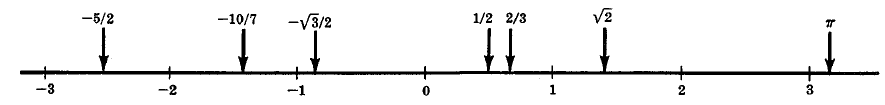
\includegraphics[width=.8\textwidth]{./calculo/fig-01-01--recta_numerica.png}
 % fig-01-01--recta numérica.png: 885x105 px, 120dpi, 18.73x2.22 cm, bb=0 0 531 63
 \label{fig:schaum 01 01}
\end{figure}


%%%%%%%
{Números reales}
	La unión de número racionales e irracionales se le conoce como \emph{números reales} $\R$.

%%%%%%%
\subsection{Orden}

	Los números reales se clasifican en
	\begin{itemize}
		\item Positivos $\set{x\in \R| x>0}$ 
		\item Cero $\set{0\in \R}$ 
		\item Negativos $\set{x\in \R | x<0}$
	\end{itemize}

%%%%%%%

 Diremos que $b\in \R$ es mayor que $a\in\R$ si $b-a>0$. 
  
 
 En ese caso escribimos $b>a$.

%%%%%%%
{}
	Diremos que $a\in \R$ es menor que  $b\in\R$ si $a-b<0$.
	
	En ese caso escribimos $a<b$.

%%%%%%%
{}
	\begin{proposicion}
		\begin{align*}
		b>a \iff a<b	
		\end{align*}
	\end{proposicion}

%%%%%%%
{Desigualdades}
	\begin{proposicion}
		Sean $a,b\in\R$. Entonces se cumple una y solo una de las siguientes condiciones:
		\begin{itemize}
			\item $a>b$
			\item $a=b$
			\item $a<b$
		\end{itemize}
	\end{proposicion}

%%%%%%%
\subsection{Reglas de álgebra}
%\subsection{Axiomas}

	Para cualesquiera $a,b,c\in\R$, se tienen las siguientes propiedades:

%%%%%%%
{}
	\begin{axioma}[Conmutatividad de la suma]
		\label{axiom--1}
		\begin{align*}
		a+b=b+a
		\end{align*}
	\end{axioma}

%%%%%%%
{}
	\begin{axioma}[Asociatividad de la suma]
		\label{axiom--2}
		\begin{align*}
	(a+b)+c = a+(b+c)
		\end{align*}
	\end{axioma}

%%%%%%%
{}
	\begin{axioma}[Conmutatividad del producto]
		\label{axiom--3}
		\begin{align*}
		ab=ba
		\end{align*}
	\end{axioma}

%%%%%%%

{}
	\begin{axioma}[Asociatividad del producto]
		\label{axiom--4}
		\begin{align*}
		(ab)c = a(bc)
		\end{align*}
	\end{axioma}

%%%%%%%
{}
	\begin{axioma}[Ley de la distribución]
		\label{axiom--5}
		\begin{align*}
		a(b+c)=ab+ac
		\end{align*}
	\end{axioma}

%%%%%%%
{Leyes de los exponentes}
	\begin{itemize}
		\item $a^{m}\cdot a^{n} = a^{m+n}$ 
		\item $\dfrac{a^{m}}{a^{n}} = a^{m-m}, a\neq 0$ 
		\item $\left(a^{m}\right)^{n} = a^{mn}$
	\end{itemize}


	\begin{itemize}
		\item $ a^{1}= a $ 
		\item $ a^{0}= 1 $ 
		\item $ a^{-1}= \dfrac{1}{a} $ 
		\item $ a^{n}= \dfrac{1}{a^{n}}  $
		\item $ a^{p/q}= \sqrt[q]{a^{p}} $
	\end{itemize}

\subsection{Ejemplos}

{}
 \begin{problema}
 	Demuestra que $\sqrt{2}$ es un número irracional.
 \end{problema}

%%%%%%%
{Solución}
	Procedamos por contradicción: 
	\begin{enumerate}
		\item Supongamos que $\sqrt{2}=\dfrac{p}{q}$ con $ p,q \in \Z$ positivos y primos relativos.  
		\item Entonces $ 2= \dfrac{p^{2}}{q^{2}}$, de manera que $p^{2}=2q^{2}$.
		\item De manera que $p$ es par, es decir, existe un entero $m$ tal que $p=2m$. 
		\item Sustituyendo obtenemos que $q^{2}=2m^{2},$ de manera que $q$ también es par. 
		\item Pero por hipótesis, $p$ y $q$ son primos relativos, de manera que no pueden ser ambos pares. $\qed$
	\end{enumerate}


%%%%%%%
{}
	\begin{problema}
		¿Qué número es más grande: $\sqrt{2}$ o $ \sqrt[3]{3} $?
	\end{problema}

%%%%%%%
{Solución}
	Procedamos por contradicción:
	\begin{enumerate}
		\item 
		Supongamos que $ \sqrt{2} \geq \sqrt[3]{3}$. 
		\item Elevamos ambos lados a la sexta potencia. 
		\item De donde obtenemos que 
		\begin{align*}
			2^{3} \geq 3^{2} \qed
		\end{align*} 
	\end{enumerate}

%%%%%%%
{}
	\begin{problema}
		Con base en los axiomas \eqref{axiom--1}-\eqref{axiom--5}, demostrar que
		\begin{align*}
			(b+c)a=ba+ca
		\end{align*}
	\end{problema}

%%%%%%%
{Solución}
		\begin{align*}
		(b+c)a &= a(b+c)\\ 
		&=ab+ac \\ 
		&=ba+ca
		\end{align*}


\section{Funciones reales}

\subsection{Definición}
{}
  Una \emph{función} $f$ es una regla que asigna a cada elemento $x$ de un conjunto $A$ un único elemento $y$ de otro conjunto $B$. 
  
  En ese caso escribiremos $f:A \to B$

%%%%%%%%%%%%%%%%%%%%%
{}
\begin{enumerate}[(i)]
  %NUEVO ITEM
  \item 
  Para indicar dicha correspondencia escribimos $y=f(x)$ y decimos que $y$ es el \emph{valor} de $f$ en $x$. 
  \item Al conjunto $A$ se le conoce como dominio. 
  \item Mientras que al conjunto $B$, se le conoce como contradominio.
\end{enumerate}

%%%%%%%%%%%%%%%%%%%%%
{}
  \begin{problema}
   Evaluar $f(x)=x^{2}-3x+2$ en $x=2$
  \end{problema}

  \begin{proof}[Solución]
     \begin{align*} 
	f(2) &= (2)^{2}-3(2)+2 \\
   &=  0
   \end{align*}
  \end{proof}

%%%%%%%%%%%%%%%%%%%%%
{}
  \begin{definicion}
   La \emph{gráfica} de una función $f: A \to B$ es el conjunto 
       \begin{align*}    
   \Gamma_{f} = \sett{\left( a,b \right)\in A\times B}{b=f(a)}
    \end{align*}
  \end{definicion}


%%%%%%%%%%%%%%%%%%%%%
{}
\begin{enumerate}[(i)]
  %NUEVO ITEM
  \item 
  En el caso $A=B=\R^{n}$, diremos que la gráfica de $F:\R \to \R$ es una \emph{curva}. 
  
  \item Diremos que $x\in A$ es la variable \emph{independiente},  mientras que $y\in B$ es la variable \emph{dependiente}.
\end{enumerate}

%%%%%%%%%%%%%%%%%%%%%
\subsection{Polinomios}
 
     \begin{align*}
   f(x) = a_{n}x^{n}+a_{n-1}x^{n-1}+...+a_{0}
   \end{align*}
    
   Si $a_{n}\neq 0$, diremos que $n$ es el grado del polinomio y $a_{n}$, su coeficiente líder. 
   
   
   Denotaremos el grado del polinomio $f$ por $\mathrm{grd}(f)$.

%%%%%%%%%%%%%%%%%%%%%
{}
Si $\mathrm{grd}(f)=n$, la ecuación polinomial $f(x)$ tiene exactamente $n$ raíces (posiblemente repetidas).


\begin{problema}
 Como $x^{3}-3x^{2}+3x-1=0$, se puede reescribir como $(x-1)^{3}$,  entonces la ecuación tiene una raíz $x=1$ repetida 3 veces. 
\end{problema}


%%%%%%%%%%%%%%%%%%%%%
{Teorema del Binomio}
  
     \begin{align*}
   \left( a+x \right)^{n} = 
   a^{n}+\binom{n}{1}a^{n-1}x+\binom{n}{2}a^{n-2}x^{2}+...+x^{n}
   \end{align*}

donde $\binom{n}{k}=\dfrac{n!}{k!\left( n-k \right)!}$

%%%%%%%%%%%%%%%%%%%%%
\subsection{Exponenciales y logaritmos}
{Funciones exponenciales}
     \begin{align*}
   \exp_{a}(x) = a^{x}, a> 0
   \end{align*}
   

%%%%%%%%%%%%%%%%%%%%%
{Leyes de los exponentes}

        \begin{align*}
    \exp_a(m+n) &= 
     \exp_{a}(m)\cdot \exp_{a}(n) \\
     \exp_a(m-n) &=    
     \dfrac{\exp_a(m)}{\exp_a(n)}     \\
     \exp_a(nm) &=      
     \left( \exp_a(m)\right)^{n}  \\       
     \exp_a(0) &=  1 \\     
     \exp_a(1) &=  a     
     \end{align*}

%%%%%%%%%%%%%%%%%%%%%
{Logaritmos}
  La función logarítmica $f(x)=\log_{a}(x)$ es la función inversa de $g(x) = \exp_{a}(x)$, 
   es decir 
       \begin{align*}
    \forall x \in \R: \log_{a}\left( \exp_{a}(x) \right) = x
    \end{align*}
    
         \begin{align*}
     \forall x \in \R^{+}: \exp_{a}\left( \log_{a}(x) \right) = x
     \end{align*}

%%%%%%%%%%%%%%%%%%%%%
{Leyes de los logaritmos}
     \begin{align*}
   \log_{a}(mn)&= \log_{a}(m)\cdot \log_{a}(n) \\
   \log_{a}\left( \dfrac{m}{n} \right)&= \log_{a}(m)-\log_{a}(n) \\ 
   \log_{a}(m^{p}) &= p\log_{a}(m) \\ 
   \log_{a}(1)&= 0\\ 
   \log_{a}(a)&=1
   \end{align*}

%%%%%%%%%%%%%%%%%%%%%
{Logaritmo natural}
  En el caso de que la base sea la constante de Euler, es decir $a=e\approx 2.718$, entonces reescribimos
     \begin{align*}
   \exp_{e}(x)=\exp(x)\\ 
   \log_{e}(x)=\ln(x)
   \end{align*}
   
   Esta última función se conoce como \emph{logaritmo natural}.

%%%%%%%%%%%%%%%%%%%%%
\subsection{Funciones trigonométricas}
{Relaciones fundamentales}
\begin{align*}
\sin(x) &=\cos\left( \dfrac{\pi}{2}-x \right) \\    
\cos(x) &= \sin\left( \dfrac{\pi}{2}-x \right) \\    
\tan(x) &= \dfrac{\sin(x)}{\cos(x)} \\     
\cot(x) &= \dfrac{\cos(x)}{\sin(x)}=\dfrac{1}{\tan(x)} \\    
\sec(x) &= \dfrac{1}{\cos(x)} \\    
\csc(x) &= \dfrac{1}{\sin(x)}
\end{align*}

%%%%%%%%%%%%%%%%%%%%%
\subsection{Identidades pitagóricas}
\begin{align*}
\sin^{2}(x)+\cos^{2}(x)&= 1\\ 
\sec^{2}(x)-\tan^{2}(x)&= 1\\ 
\csc^{2}(x)-\cot^{2}(x)&= 1
\end{align*}

%%%%%%%%%%%%%%%%%%%%%
{Paridad}
     \begin{align*}
   \sin(-x) &= -\sin(x) \\ 
   \cos(-x) &= \cos(x) \\ 
   \tan(-x) &= -\tan(x) 
   \end{align*}

%%%%%%%%%%%%%%%%%%%%%
{Sumas de ángulos}
     \begin{align*}
   \sin(x\pm y) &= \sin(x)\cos(y)\pm\cos(x)\sin(y) \\   
   \cos(x\pm y) &= \cos(x)\cos(y)\mp\sin(x)\sin(y) \\   
   \tan(x\pm y) &= \dfrac{\tan(x)\pm \tan(y)}{1+\mp \tan(x)\tan(y)}
   \end{align*}

%%%%%%%%%%%%%%%%%%%%%
{Ondas sinusoidales}
     \begin{align*}
   \begin{cases}
A\cos(x)+B\sin(x) = \sqrt{A^{2}+B^{2}}\sin(x+\alpha)\\
\tan(\alpha) = \dfrac{A}{B}
\end{cases}
   \end{align*}

%%%%%%%%%%%%%%%%%%%%%
{Periodicidad}
  Las funciones $\sin(x)$ y $\cos(x)$ tiene periodo $T=2\pi$.   
  Mientras que la función $\tan(x)$ tiene periodo $T=\pi$.
  
  
%%%%%%%%%%%%%%%%%%%%%
{Inversas trigonométricas}
   Las funciones inversas de funciones trigonométricas estás sólo definidas \emph{localmente}:  Por ejemplo,
      \begin{align*}
     y = \sin(x) \iff x =\sin^{-1}(y)
     \end{align*} 
     siempre y cuando 
          \begin{align*}
      x\in\left[-\dfrac{\pi}{2}, \frac{\pi}{2} \right],
      y\in\left[ -1,1 \right]
      \end{align*}

%%%%%%%%%%%%%%%%%%%%%
\subsection{Funciones hiperbólicas}
{Relaciones fundamentales}
 \begin{align*}
\sinh(x) &= \dfrac{e^{x}-e^{-x}}{2}\\ 
\cosh(x) &= \dfrac{e^{x}+e^{-x}}{2}
\end{align*}

%%%%%%%%%%%%%%%%%%%%%
{}
\begin{align*}
\tanh(x) &= \dfrac{\sinh(x)}{\cosh(x)}\\ 
&=\dfrac{e^{x}-e^{-x}}{e^{x}+e^{-x}}
 \end{align*}  

%%%%%%%%%%%%%%%%%%%%%
{}
\begin{align*}
\coth(x) &= \dfrac{\cosh(x)}{\sinh(x)}\\ 
& = \dfrac{1}{\tanh(x)}\\ 
& = \dfrac{e^{x}+e^{-x}}{e^{x}-e^{-x}} 
\end{align*}

%%%%%%%%%%%%%%%%%%%%%
{}
 \begin{align*}
\sech(x)&= \dfrac{1}{\cosh(x)} \\ 
&= \dfrac{2}{e^{x}+e^{-x}}
\end{align*}

%%%%%%%%%%%%%%%%%%%%%
{}
\begin{align*}
\csch(x)&= \dfrac{1}{\sinh(x)} \\ 
&= \dfrac{2}{e^{x}-e^{-x}}
\end{align*}

%%%%%%%%%%%%%%%%%%%%%
{Identidades pitagóricas}
\begin{align*}
\cosh^{2}(x)-\sinh^{2}(x)&= 1\\
\sech^{2}(x)+\tanh^{2}(x)&= 1\\
\coth^{2}(x)-\csch^{2}(x)&= 1
\end{align*}

%%%%%%%%%%%%%%%%%%%%%
{Sumas de ángulos}
 \begin{align*}
\sinh(x\pm y) &= \sinh(x)\cosh(y)\pm \cosh(x)\sinh(y)\\
\cosh(x\pm y) &= \cosh(x)\cosh(y)\pm \sinh(x)\sinh(y)\\
\tanh(x\pm y) &= \dfrac{\tanh(x)\pm \tanh(y)}{1\pm \tanh(x)\tanh(y)}
\end{align*}

%%%%%%%%%%%%%%%%%%%%%
\subsection{Ejemplos}
{}
\begin{problema}
\label{solved 1.4}
Si $f(x)=2x^{2}-3x+5$, encontrar
\begin{enumerate}[(i)]
 %NUEVO ITEM     
 \item $f(h)-f(0)$
 
 \item $f(h-1)-f(-1)$
 
 \item $f(x+h)$
 
 \item $f(x+h)-f(x)$
 
 \item $\dfrac{f(x+h)-f(x)}{h}$
\end{enumerate}
\end{problema}


%%%%%%%%%%%%%%%%%%%%%
{}
  \begin{problema}
   \label{solved 1.5}
   Usando las leyes de los exponentes, demostrar las leyes de los logaritmos.
  \end{problema}


%%%%%%%%%%%%%%%%%%%%%
{}
  \begin{problema}
   \label{solved 1.6}
   Demostrar que 
   \begin{enumerate}[(i)]
     %NUEVO ITEM
     \item $\sin^{2}(x)=\dfrac{1}{2}\left( 1-\cos(2x) \right)$ 
     
     \item $\cos^{2}(x)=\dfrac{1}{2}\left( 1+\cos(2x) \right)$
\end{enumerate}
  \end{problema}


%%%%%%%%%%%%%%%%%%%%%
{}
  \begin{problema}
   \label{solved 1.7}
   Demostrar que \[A \cos(x) + B\sin(x) = \sqrt{A^{2}+B^{2}}\sin(x+\alpha)\] donde $\tan(\alpha)=\dfrac{A}{B}$.
  \end{problema}


%%%%%%%%%%%%%%%%%%%%%
{}
  \begin{problema}
   \label{solved 1.8}
   Demostrar que 
   \begin{enumerate}[(i)]
     %NUEVO ITEM
     \item $\cosh^{2}(x)-\sinh^{2}(x)=1$       
     \item $\sech^{2}(x)+\tanh^{2}(x)=1$
\end{enumerate}
  \end{problema}


%%%%%%%%%%%%%%%%%%%%%
{}
  \begin{problema}
   \label{solved 1.9}
   Demostrar que $\cosh^{-1}(x)=\pm \ln\left( x+\sqrt{x^{2}-1} \right)$
  \end{problema}


%%%%%%%%%%%%%%%%%%%%%


\chapter{Sistemas lineales}

%402
\section{Sistemas de Ecuaciones Lineales Simultáneas}

\subsection{Sistemas de Dos Ecuaciones Lineales}

 Supongamos que $a_{i}, b_{i}, c_{i}, i=1,2$ son número dados:
	$$\begin{cases}
		a_{1}x+b_{1}y=c_{1}\\
		a_{2}x+b_{2}y=c_{2}\\
	\end{cases}
	$$
	En el sistema anterior, nuetro objetivos es encontrar dos números $x,y$ tales que cumplan ambas ecuaciones simultaneamente.



	\begin{problema}
		La soluci\'on del sistema 
		$$\begin{cases}
			x+y=7\\
			x-y=3
		\end{cases}
		$$ es $x=5,y=2.$
	\end{problema}
	



	A continuaci\'on, ejemplificaremos algunos de los m\'etodos más comunes para resolver sistemas de ecuaciones.

%

\[
	\label{spi151}
	2x-y=4
\]
\[	
	\label{spi152}
	x+2y=-3
\]		

	


{M\'etodo de sustituci\'on} 
	Despejando de \eqref{spi151}, obtenemos
	$$y=2x-4.$$
	
	Sutituyendo en \eqref{sp152}, obtenemos
	$$
	x+2(2x-4)=-3.
	$$
	


{M\'etodo de igualaci\'on}
	Despejando de \eqref{spi151}, obtenemos
	$$y=2x-4.$$
	
	Despejando de \eqref{sp152}, obtenemos
	$$y=-\dfrac{3+x}{2}.$$
	
	Igualando ambos lados derechos, obtenemos
	$$
	2x-4=-\dfrac{3+x}{2}.
	$$



{M\'etodo gráfico}
	\begin{figure}
		\centering
		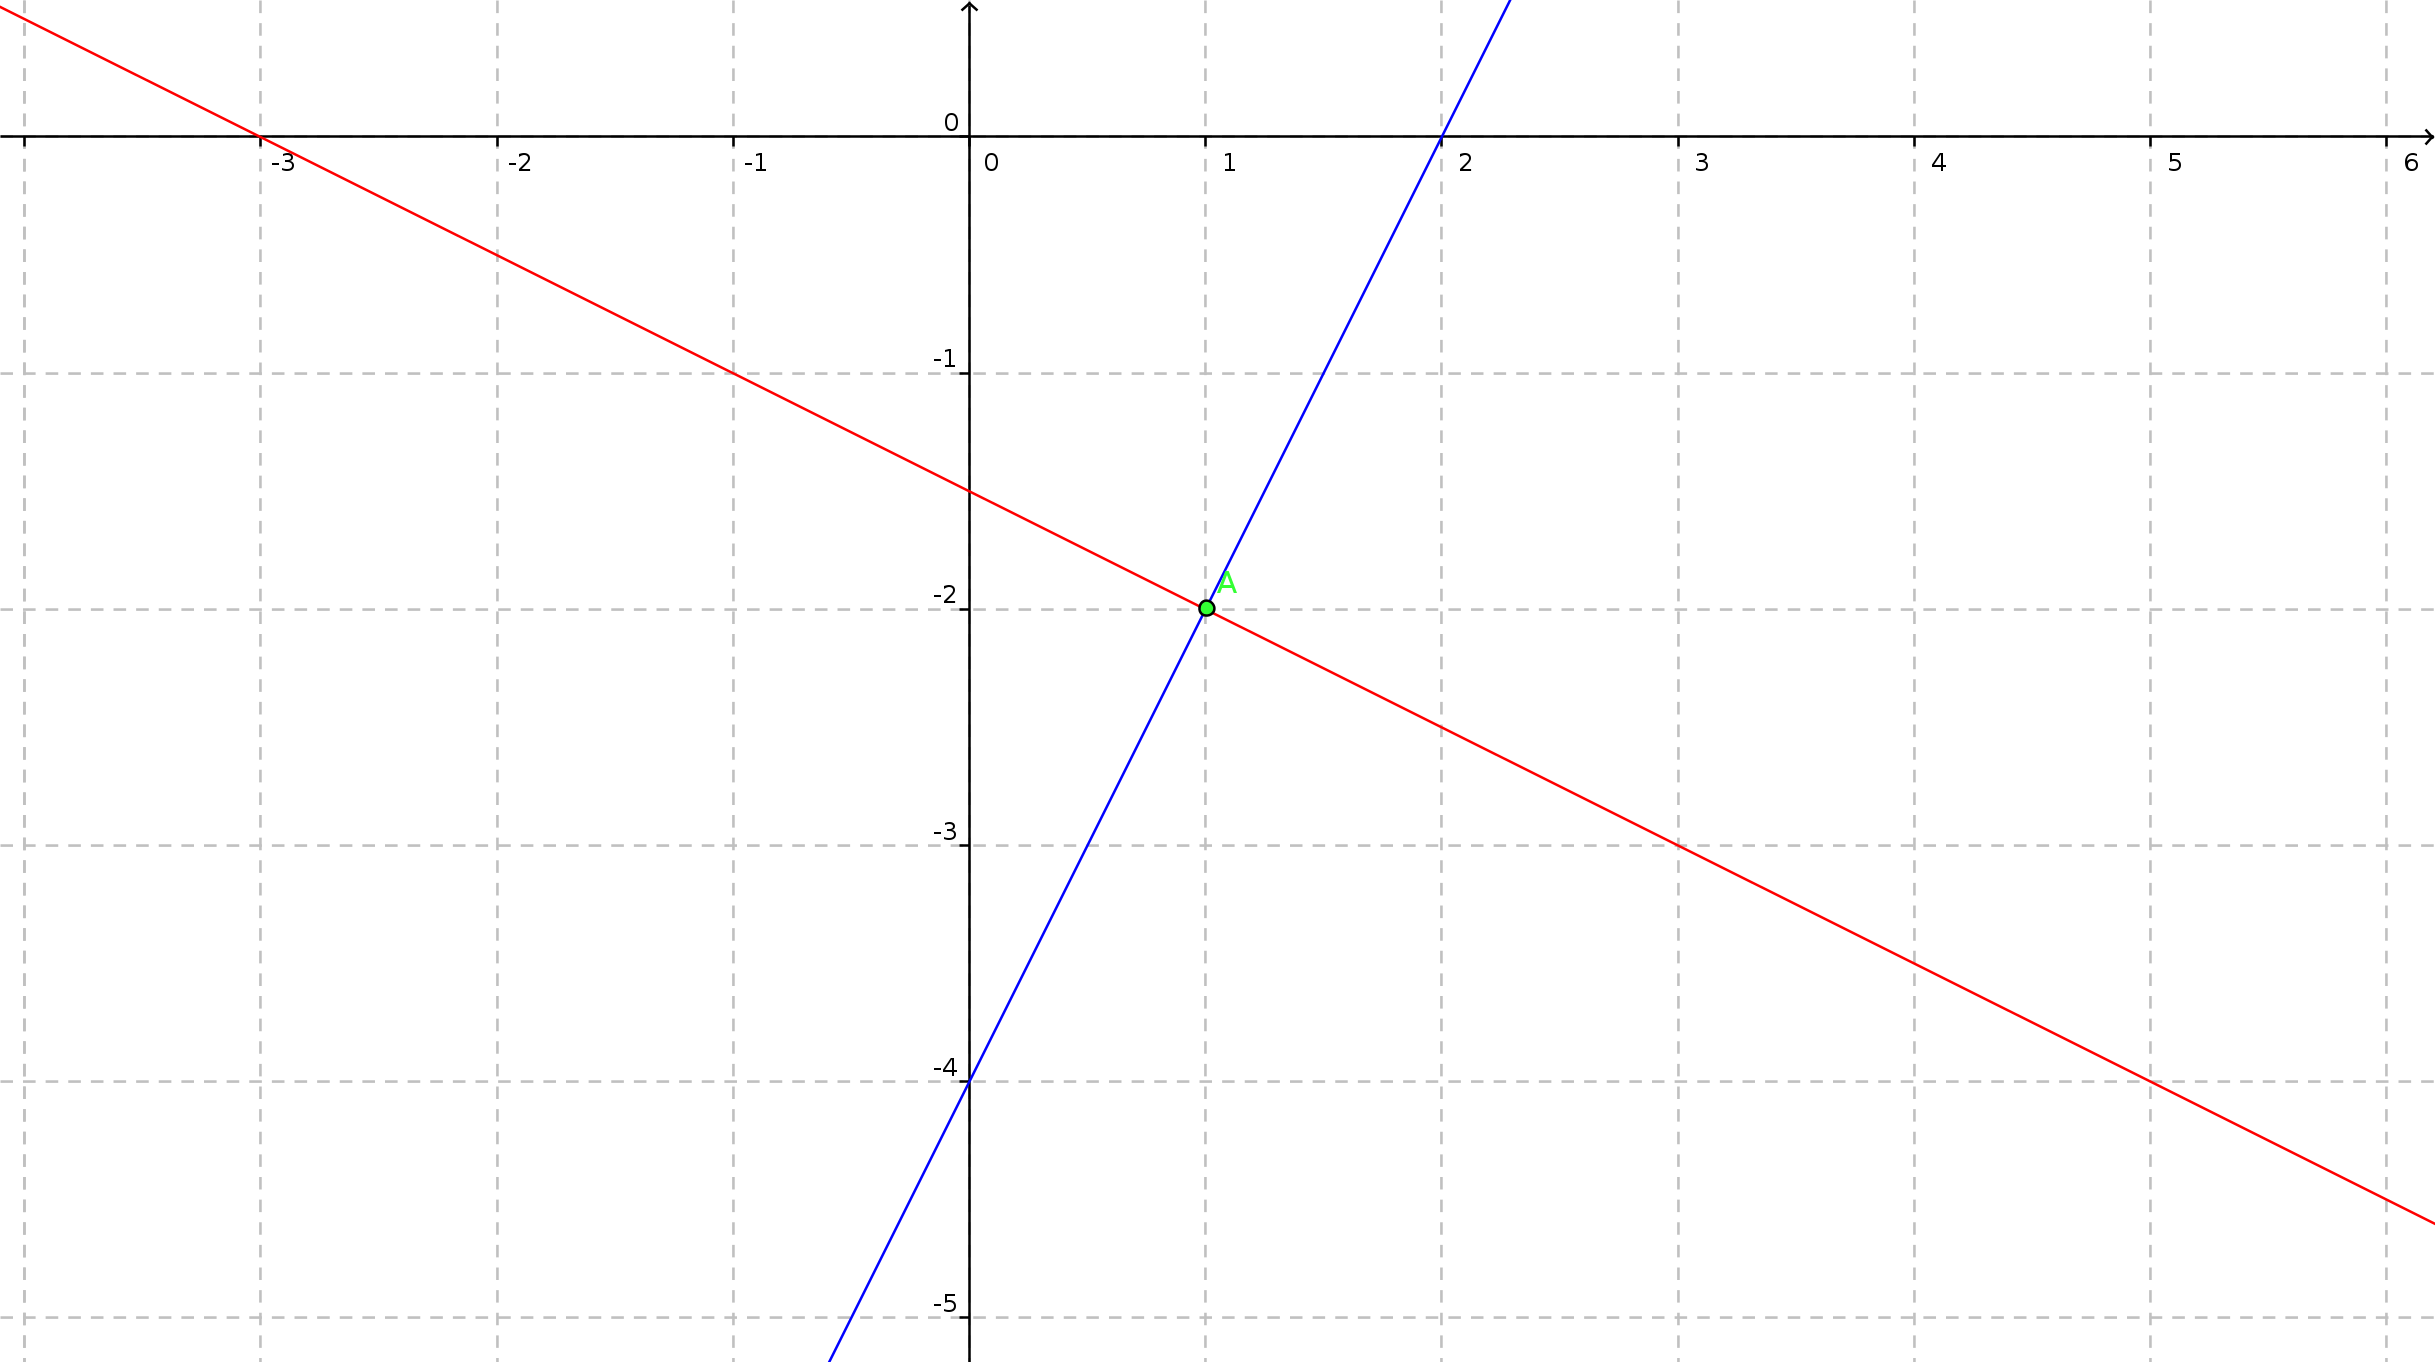
\includegraphics[height=5cm,keepaspectratio=true]{./precalculo/IM0401.png}
		% IM0401.png: 0x0 pixel, 300dpi, 0.00x0.00 cm, bb=
		\caption{$$2x-y=4\, , x+2y=-3$$}
		\label{fig:IM0401}
	\end{figure}
	


{Tipos de sistemas}
	\begin{figure}
		\centering
		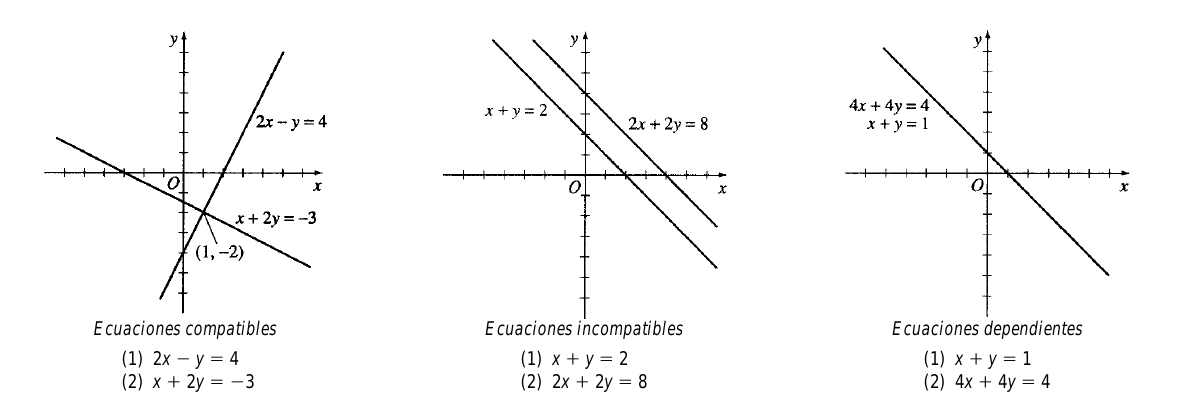
\includegraphics[width=12cm,keepaspectratio=true]{./precalculo/IM0402.png}
		% IM0402.png: 0x0 pixel, 300dpi, 0.00x0.00 cm, bb=
		\label{fig:0401}
	\end{figure}
	



%403
\section{Determinantes}

\subsection{Determinantes de Segundo Orden}

{Definición}
	\begin{definicion}
		$$
		\begin{vmatrix}
			a & b \\ c & d
		\end{vmatrix}=ad-bc.
		$$
	\end{definicion}
	



	\begin{problema}
		$$
		\begin{vmatrix} 2 & 3 \\ -1 & -2 \end{vmatrix}=
		$$
	\end{problema}
	



	Si consideremos el siguiente sistema de ecuaciones
	\[
		\begin{cases}
			a_{1}x+b_{1}y=c_{1}\\
			a_{2}x+b_{2}y=c_{2}
		\end{cases}...
	\]
	



	...y definimos
	\begin{align*}
		\Delta&=\begin{vmatrix} a_{1} & b_{1} \\ a_{2} & b_{2} \end{vmatrix}\\
		\Delta_{x}&=\begin{vmatrix} c_{1} & b_{1} \\ c_{2} & b_{2} \end{vmatrix}\\
		\Delta_{y}&=\begin{vmatrix} a_{1} & c_{1} \\ a_{2} & c_{2} \end{vmatrix}...
	\end{align*}



	...entonces
	\[
		\label{spi:28.2}
		\begin{split}
			x&=\dfrac{\Delta_{x}}{\Delta}\\
			y&=\dfrac{\Delta_{y}}{\Delta}
		\end{split}
	\]
	



	\begin{problema}
		Resuelva el sistema
		$$\begin{cases}
			2x+3y=8\\
			x-2y=-3
		\end{cases}
		$$
	\end{problema}
	

\subsection{Ejemplos}


	El m\'etodo de soluci\'on de sistemas de ecuaciones linales, por medio de determinantes, se conoce como Regla de Cramer.



	\begin{problema} Resuelva el siguiente sistema por la Regla de Cramer
		\label{spi:28.4a}
		$$
		\begin{cases}
			4x+2y=5\\
			3x-4y=1
		\end{cases}
		$$
	\end{problema}
	



	\begin{problema} Resuelva el siguiente sistema por la Regla de Cramer
		\label{spi:28.4b}
		$$
		\begin{cases}
			3u+2v=18\\
			-5u-v=12
		\end{cases}
		$$
	\end{problema}
	


\subsection{Sistemas Indeterminados}


	Un sistema de $ n $ ecuaciones con $ n $ incognitas tiene una única solución si y solo si su determinante principal $ \Delta \neq 0. $  
	
	En este caso, decimos que el sistema es consistente.



	Si $ \Delta =0 $, entonces o bien existen multiples soluciones, o bien no existe alguna en absoluto.
	
	En cualquier caso, decimos que el sistema es inconsistente.



	Determine si 
	$$\begin{cases}
		5x-2y=10\\
		10x-4y=20
	\end{cases}$$
	es consistente; y de no ser el caso, explique que sucede con las soluciones.



	Determine si 
	$$\begin{cases}
		5x+3y=15\\
		10x+6y=60
	\end{cases}$$
	es consistente; y de no ser el caso, explique que sucede con las soluciones.




\subsection{Ejemplos}


	\begin{problema}
		\begin{align*}
			2x-y&=4\\
			x+y&=5
		\end{align*}
		
	\end{problema}
	



	\begin{problema}
		\begin{align*}
			5x+2y&=3\\
			2x+3y&=-1
		\end{align*}
		
	\end{problema}
	



	\begin{problema}
		\begin{align*}
			2x+3y=3\\
			6y-6x=1
		\end{align*}
		
	\end{problema}
	



	\begin{problema}
		\begin{align*}
			5y&=3-2x\\
			3x&=2y+1
		\end{align*}
		
	\end{problema}
	



	\begin{problema}
		\begin{align*}
			\dfrac{x-2}{3}+\dfrac{y+1}{6}=2\\
			\dfrac{x+3}{4}-\dfrac{2y-1}{2}=1
		\end{align*}
		
	\end{problema}
	



\chapter{Polinomios}


%201
\section{Reducci\'on de t\'erminos semejantes}

 En el álgebra, representamos cantidades desconocidas por s\'imbolos;  generalmente son letras como $x,y,z,$ pero \emph{no debe olvidarse que respresentan números.}



	Para representar una multiplicaci\'on iterada, usamos el s\'imbolo de potencia
	$$
	x^{n}=\underbrace{x\cdot\cdots \cdot x}_{n\texttt{-veces}};
	$$
	al número $x$ le llamamos base y al número $n$ le llamamos potencia.



	\begin{problema}
		\begin{enumerate}
			\item $3^{2}=3\cdot3=9$
			\item $5^{3}=5\cdot5\cdot5=125$
			\item $2^{4}=2\cdot2\cdot2\cdot2=16$
		\end{enumerate}
		
	\end{problema}
	



	\begin{problema}
		\begin{enumerate}
			\item $x^{2}=x\cdot x$
			\item $x^{3}=x\cdot x\cdot x$
			\item $x^{4}=x\cdot x\cdot x\cdot x$
			\item $\cdots$
		\end{enumerate}
		
	\end{problema}




	\begin{observacion}
		Observe que $x^{1}=x;$ mientras que, por convenci\'on, $x^{0}=1.$
	\end{observacion}
	



	Cuando multiplicamos $x^{n}$ por un número diferente de $x:$
	$$ax^{n}=a\cdot\underbrace{x\cdot\cdots *x},$$ diremos que $a$ es el coeficiente de $x^{n}.$ 



	A un número escrito en la forma $ax^{n}$ se le llama \emph{monomio;} y diremos que dos monomios son semejantes si tienen \emph{exactamente} la misma base a la misma potencia.



	\begin{problema}
		Determine cual de los siguientes monomios es semejante a $2x^{3}:$
		\begin{enumerate}
			\item $3x^{3};$
			\item $2x^{2};$
			\item $2y^{3};$
		\end{enumerate}
		
	\end{problema}
	



	Dos t\'erminos semejantes pueden reducirse 
	$$\begin{cases}
		ax^{n}+bx^{n}=\left( a+b \right)x^{n}\\
		ax^{n}-bx^{n}=\left( a-b \right)x^{n}
	\end{cases}
	$$



	\begin{problema}
		Reduzca los siguientes t\'erminos semejantes, escribiendo el coeficiente en forma irreducible.
		\begin{enumerate}
			\item $\left( 4n^{2}+5n+3 \right)+\left( -3n^{2}-2n \right)$
			\item $\left( -7a^{3}-a^{2}-5a-2 \right)+\left( a^{3}+a^{2}-4a+7 \right)$
			\item \begin{eqnarray*}
				\left(5u^{5}-3u^{4}+2u^{3}-5u^{2}+7u-7\right)+ \\
				\left( \dfrac{2u^{5}}{3}+\dfrac{3u^{4}}{2}-\dfrac{2u^{2}}{3}+\dfrac{5u}{6}+\dfrac{5}{4} \right).
			\end{eqnarray*}
			
		\end{enumerate}
		
	\end{problema}
	



	\begin{problema}
		Reduzca los siguientes t\'erminos semejantes, escribiendo el coeficiente en forma irreducible.
		\begin{enumerate}
			\item $\left( 4n^{2}+5n+3 \right)-\left( -3n^{2}-2n \right)$
			\item $\left( -7a^{3}-a^{2}-5a-2 \right)-\left( a^{3}+a^{2}-4a+7 \right)$
			\item \begin{eqnarray*}
				\left(5u^{5}-3u^{4}+2u^{3}-5u^{2}+7u-7\right)- \\
				\left( \dfrac{2u^{5}}{3}+\dfrac{3u^{4}}{2}-\dfrac{2u^{2}}{3}+\dfrac{5u}{6}+\dfrac{5}{4} \right).
			\end{eqnarray*}
			
		\end{enumerate}
		
	\end{problema}
	



	\begin{observacion}
		A la suma de dos o más monomios se le conoce como \emph{polinomio}.
		
		Por ejemplo $x^{2}-2x+1$ o $x^{2}-2xy+y^{2}.$
		
	\end{observacion}
	



%202
\section{Supresi\'on de signos de agrupaci\'on}


	Cuando queremos quitar parentesis u otro signo de agrupaci\'on, en una suma o resta de polinomios, basta usar la regla de los signos.



	Sin embargo, cuando un polinomio se multiplica por un coeficiente, se utiliza la siguiente regla
	\begin{proposicion}[Ley de la distribuci\'on]
		\begin{eqnarray}
			\label{distribucion}
			a\left( b+c \right)=ab+ac\\
			\left( a+b \right)\left( c+d \right)=ac+ad+bc+bd.
		\end{eqnarray}
		
	\end{proposicion}
	



	\begin{problema} Simplifique
		\begin{enumerate}
			\item $(6-7a)(2-4a)$
			\item $-4(-4w-5)(4w-2)$
			\item $6(-5v-7)(4-5v)(-2v-1)v$
		\end{enumerate}	
	\end{problema}
	



%203
\section{Mutiplicaci\'on de polinomios}


	Dos monomios se pueden multiplicar de la siguiente manera
	$$
	(ax^{n})(bx^{m})=(ab)x^{n+m}.
	$$



	\begin{problema}
		\begin{enumerate}
			\item $\left( 2x^{3} \right)\left( 3x^{2} \right)=\left( 2*3 \right)x^{2+3}=6x^{5}.$
		\end{enumerate}
		
	\end{problema}
	



	\begin{problema}
		Exprese su respuesta en la forma más simple posible:
		\begin{enumerate}
			\item $(6x^{4})(4-3x-3x^{2})$
			\item $5w^{3}\left( -7w^{3}-7w^{2}+7w+3 \right)$
			\item $\dfrac{a^{3}}{3}\left( -7a^{5}-2a^{4}+3a^{3}+a^{2}-a-3 \right)$
		\end{enumerate}
		
	\end{problema}
	



	\begin{problema}
		Exprese su respuesta en la forma más simple posible:
		\begin{enumerate}
			\item $$
			\left( n^{2}+5n \right)
			\left( -n^{2}+6n+1 \right)
			$$
			
			\item $$
			\left( -6a^{2}-3a-7 \right)
			\left( a^{3}+a^{2}+6a-7 \right)
			$$
			
			\item $$
			\left( \dfrac{9w^{4}}{8}+\dfrac{8w^{3}}{9}-\dfrac{7w^{2}}{9}-\dfrac{w}{3}+\dfrac{5}{9} \right)
			\left( -2w^{3}-5w+7 \right)
			$$
		\end{enumerate}
		
	\end{problema}
	



	\begin{problema}
		Exprese su respuesta en la forma más simple posible:
		\begin{enumerate}
			\item $(7u^4)\left( 6-4u-7u^{2} \right)$ 
			\item $(3s^{4})\left( -7+s-s^{2}-5s^{3} \right)$
			\item $(7x^{4})\left( 2+4x-7x^{2} \right)$
		\end{enumerate}
	\end{problema}



	\begin{problema}
		Simplifique
		\begin{enumerate}
			\item $(5w^{4})\left( -1+5w+4w^{2}+6w^{3} \right)$
			\item $(3m^{4})\left( -1-6m-3m^{2}-7m^{3}-4m^{4} \right)$
			\item $5a^{5}\left( a^{3}-3a^{2}+3a-5 \right)$
		\end{enumerate}
		
	\end{problema}
	
	



	\begin{problema}
		Escriba su respuesta de la forma más simple posible
		\begin{enumerate}
			\item $\left( \dfrac{8n^{4}}{9} \right)\left( n^{4}-3n^{3}-4n^{2}+3n-1 \right)$
			\item $\left( \dfrac{2y^{5}}{5} \right)\left( -3y^{4}+5y^{3}-7y^{2}-2y-5 \right)$
			\item $\left( \dfrac{3s^{3}}{7} \right)\left( -2s^{4}-s^{3}-5s^{2}+2s+1 \right)$
		\end{enumerate}
		
	\end{problema}
	



	\begin{problema}
		Exprese su respuesta en la forma más simple posible
		\begin{enumerate}
			\item $\left( -4x-5 \right)\left( -3x^{3}+3x^{2}-4x-4 \right)$
			\item $\left( 6y-7y^{2} \right)\left( y+3 \right)$
			\item $\left( \dfrac{7w^{2}}{9}+\dfrac{4w}{9}+\dfrac{9}{2} \right)\left( 5w^{2}+6w-7 \right)$
		\end{enumerate}
		
	\end{problema}
	



	\begin{problema}
		Simplifique
		\begin{enumerate}
			\item $\left( 3x^{2}+2x+3 \right)\left( 6x^{2}-4x-3 \right)$
			\item $\left( 4m^{2}+3m \right)\left( 6m^{3}+6m^{2}-7m+6 \right)$
			\item $\left( -4x^{2}+5x+5 \right)\left( 3-4x \right)$
			
		\end{enumerate}
		
	\end{problema}
	



	\begin{problema}
		Simplifique
		\begin{enumerate}
			\item $\left( -2s^{4}-5s^{3}+3s^{2}+3s+2 \right)\left( 7s^{3}-3s^{2}-2s-7 \right)$
			\item $\left( 5v-v^{2} \right)\left( 2v^{2}+6v+5 \right)$
			\item $\left( 7x^{3}+2x^{2}+5x-6 \right)\left( 6x^{3}+3x^{2}-4x-4 \right)$
		\end{enumerate}
		
	\end{problema}
	



	\begin{problema}
		Simplifique
		$$
		\left( \dfrac{2a^{3}}{5}-\dfrac{5a^{2}}{6}-\dfrac{9a}{8}+\dfrac{2}{3} \right)\left( 3a^{2}-2a-4 \right)
		$$
	\end{problema}
	

% 
% \section{División de Polinomios}
% 
% 
%  \begin{problema}
%  \label{st:3.2.1}
%   Divida $6x^{2}-26x+12$ entre $x-4.$ Compruebe.
%  \end{problema}
% 
% 
% 
% 
%  \begin{proof}[Soluci\'on]
%   $$6x^{2}-26x+12=\left( x-4 \right)\left( 6x-2 \right)+4$$
%  \end{proof}
% 
% 
% 
% 
%  \begin{problema}
%  \label{st:3.2.2}
%   Divida $8x^{4}+6x^{2}-3x+1$ entre $2x^{2}-x+2.$ Compruebe
%  \end{problema}
% 
% 
% 
% 
%  \begin{proof}[Sol.]
%   $$
%   8x^{4}+6x^{2}-3x+1=
%   \left( 2x^{2}-x+2 \right)
%   \left( 4x^{2}+2x \right)+
%   \left( -7x+1 \right)
%   $$
%  \end{proof}
% 
% 
% 
% 
%  \begin{problema}
%   Divida $2x^{3}-7x^{2}+5$ entre $x-3.$ Repita el ejericicio \emph{usando divisi\'on sint\'etica.} Compruebe.
%  \end{problema}
% 
% 
% 
% 
%  \begin{proof}[Sol.]
%   $$2x^{3}-7x^{2}+5=
%   \left( x-3 \right)
%   \left( 2x^{2}-x-3 \right)-4$$
%  \end{proof}
% 
% 
% 
% 
%  \begin{problema}
%   Realice las siguientes divisiones; comprebe.
%   \begin{enumerate}
%    \item $\dfrac{x^{2}-6x-8}{x-4}$
%    \item $\dfrac{4x^{3}+2x^{2}-2x-3}{2x+1}$
%    \item $\dfrac{x^{3}+6x+3}{x^{2}-2x+2}$
%    \item $\dfrac{6x^{3}+2x^{2}+22x}{2x^{2}+5}$
%    \item $\dfrac{x^{6}+x^{4}+x^{2}+1}{x^{2}+1}$
%   \end{enumerate}
% 
%  \end{problema}
% 
% 
% 
% 
%  \begin{problema}
%   Realice las siguientes operaciones, \emph{utilizando divisi\'on sint\'etica.} Compruebe.
%   \begin{enumerate}
%    \item $\dfrac{x^{2}-5x+4}{x-3}$
%    \item $\dfrac{3x^{2}+5x}{x-6}$
%    \item $\dfrac{x^{3}+2x^{2}+2x+1}{x+2}$
%    \item $\dfrac{x^{3}-8x+2}{x+3}$
%    \item $\dfrac{x^{5}+3x^{3}-6}{x-1}$
%   \end{enumerate}
% 
%  \end{problema}
% 
% 

%%\section{Productos Especiales}

%204
\section{Productos notables}


	A continuaci\'on, aparecen algunos de los productos que se presentan con frecuencia en matemáticas.


{Producto monomio-binomio}
	\[
		a(c+d)=ac+ad
	\]	



	\begin{problema}
		\begin{enumerate}
			\item $2xy\left( 3x^{2}y - 4y^{3}\right)$ 
			\item $3x^{2}y^{3}\left( 2xy-x-2y \right)$ 
			\item $\left( 2st^{3}-4rs^{2}+3s^{3}t \right)
			\left( 5rst^{2} \right)$
		\end{enumerate}
		
	\end{problema}
	



{Diferencia de cuadrados}
	\[
		\left( a+b \right)\left( a-b \right)
		=a^{2}-b^{2}
	\]
	



	\begin{problema}
		\begin{enumerate}
			\item $\left( 3a+5b \right)\left( 3a-5b \right)$ 
			\item $\left( 5xy+4 \right)\left( 5xy-4 \right)$ 
			\item $\left( 2-5y^{2} \right)\left( 2+5y^{2} \right)$ 
			\item $\left( 3a+5a^{2}b \right)\left( 3a-5a^{2}b \right)$
		\end{enumerate}
		
	\end{problema}
	



{Cuadrado de un binomio}
	\begin{align*}
		\left( a+b \right)^{2}&=
		a^{2}+2ab+b^{2}\\
		\left( a-b \right)^{2}&=
		a^{2}-2ab+b^{2}
	\end{align*}
	



	\begin{problema}
		\begin{enumerate}
			\item $\left( x+6 \right)^{2}$ 
			\item $\left( y+3x \right)^{2}$ 
			\item $\left( z-4 \right)^{2}$ 
			\item $\left( 3-2x^{2} \right)^{2}$  
			\item $\left( x^{2}y-2z \right)^{2}$ 
		\end{enumerate}
		
	\end{problema}
	



{Producto de dos binomios}
	\begin{align*}
		\left( x+a \right)\left( x+b \right)&=
		x^{2}+\left( a+b \right)x+ab\\
		\left( ax+b \right)\left( cx+d \right)&=
		acx^{2}+\left( ad+bc \right)x+bd
	\end{align*}
	



	\begin{problema}
		\begin{enumerate}
			\item $\left( x+2 \right)\left( x+4 \right)$ 
			\item $\left( x-4 \right)\left( x+7 \right)$ 
			\item $\left( y+3 \right)\left( y-5 \right)$ 
			\item $\left( xy+6 \right)\left( xy-4 \right)$ 
			\item $\left( 2x-3 \right)\left( 4x+1 \right)$ 
			\item $\left( 4+3r \right)\left( 2-r \right)$
		\end{enumerate}
		
	\end{problema}
	



{Cubo de un binomio}
	\begin{align*}
		\left( a+b \right)^{3}&=
		a^{3}+3a^{2}b+3ab^{2}+b^{3}\\
		\left( a-b \right)^{3}&=
		a^{3}-3a^{2}b+3ab^{2}-b^{3}
	\end{align*}
	



	\begin{problema}
		\begin{enumerate}
			\item $\left( 2x+1 \right)^{3}$ 
			\item $\left( 3x+2y \right)^{3}$ 
			\item $\left( r-2s \right)^{3}$ 
			\item $\left( x^{2}-1 \right)^{3}$ 
			\item $\left( ab^{2}-2b \right)^{3}$
		\end{enumerate}
		
	\end{problema}
	



{Cuadrado de un trinomio}
	\[
		\left( a+b+c \right)^{2}=
		a^{2}+b^{2}+c^{2}+2ab+2ac+2bc.
	\]
	



	\begin{problema}
		$$
		\left( x-2y+z \right)^{2}. 
		$$
	\end{problema}
	



%205
\section{Sumas y diferencias de potencias}


	\begin{problema}
		\begin{align*}
			\left( a-b \right)\left( a^{2}+ab+b^{2} \right)\\
			\left( a-b \right)\left( a^{3}+a^{2}b+ab^{2}+b^{3} \right)\\
			\left( a-b \right)\left( a^{4}+a^{3}b+a^{2}b^{2}+ab^{3}+b^{4} \right)
		\end{align*}
		
	\end{problema}
	



	\begin{problema}
		\begin{align*}
			\left( a+b \right)\left( a^{2}+ab+b^{2} \right)\\
			\left( a+b \right)\left( a^{3}+a^{2}b+ab^{2}+b^{3} \right)\\
			\left( a+b \right)\left( a^{4}+a^{3}b+a^{2}b^{2}+ab^{3}+b^{4} \right)
		\end{align*}
		
	\end{problema}
	



	\begin{problema}
		\begin{enumerate}
			\item $\left( t-2 \right)\left( t^{2}+2t+4 \right)$ 
			\item $\left( z-x \right)\left( x^{2}+xz+z^{2} \right)$ 
			\item $\left( x+3y \right)\left( x^{2}-3xy+9y^{3} \right)$
		\end{enumerate}
		
	\end{problema}
	



	\begin{problema}
		\begin{enumerate}
			\item $\left( s-1 \right)\left( s^{3}+s^{2}+s +1\right)$ 
			\item $\left( 1+t^{2} \right)\left( 1-t^{2}+t^{4}-t^{6} \right)$ 
			\item $\left( 3x+2y \right)^{2}\left( 3x-2y \right)^{2}$ 
			\item $\left( x^{2}+2x+1 \right)^{2}\left( x^{2}-2x+1 \right)^{2}$ 
			\item $\left( y-1 \right)^{3}\left( y+1 \right)^{3}$
			\item $(u+2)(u-2)(u^{2}+4)(u^{4}+16)$
		\end{enumerate}
		
	\end{problema}
	




\chapter{Factorización}

%301
\section{M\'etodo de Horner y Divisi\'on Sint\'etica}


	\begin{problema}
		Consideremos evaluar el siguiente polinomio
		$$
		p(x)=6x^{2}+3x-2
		$$ en $x=9.$
	\end{problema}
	



	\begin{align*}
		p(9)&=6(9)^{2}+3(9)-2  \\
		&=6(81)+3(9)-2  \\
		&=486+27-2  \\
		&=513-2=511
	\end{align*}
	



	Consideraremos una forma alternativa de evaluar, conocida como \emph{m\'etodo de Horner.}



	Primero, reescribimos el polinomio de la siguiente manera 
	\begin{align*}
		p(x)&=\left( \textcolor{blue}{6}x^{2} + \textcolor{green}{3}x \right) \textcolor{red}{-2}\\
		&= \left( \textcolor{blue}{6}x+\textcolor{green}{3} \right)x\textcolor{red}{-2} \\
		&= \left( (\textcolor{blue}{6}) x + \textcolor{green}{3} \right) x \textcolor{red}{-2}
	\end{align*}
	



	Al evaluar, realizamos las siguientes operaciones
	\begin{align*}
		p(9)&=\left( (\textcolor{blue}{6}) 9  \textcolor{green}{+3} \right) 9 \textcolor{red}{-2}\\
		&=\left( \textcolor{blue}{54} \textcolor{green}{+3} \right)9\textcolor{red}{-2} \\
		&= \left( \textcolor{green}{57} \right)9\textcolor{red}{-2}\\
		&=\textcolor{green}{513}\textcolor{red}{-2}\\
		&=\textcolor{red}{511}
	\end{align*}
	



	\begin{observacion}
		Aunque con el m\'etodo anterior, hemos realizado algunos pasos más, hemos evitado el uso de \emph{exponentes}.  Ahora, todo se reduce a \emph{multiplicaciones y sumas.}
	\end{observacion}
	



	El m\'etodo anterior se puede sintetizar de la siguiente manera
	\begin{center}
		\begin{tabular}{l|lll}
			9 & \textcolor{blue}{6} & \textcolor{green}{+3} & \textcolor{red}{-2}\\
			& $\downarrow$ & 54 & 513\\\hline
			& 6 & 57 & 511
		\end{tabular}
	\end{center}
	



	De manera general, 
	\begin{center}
		\begin{tabular}{l|lll}
			x & \textcolor{blue}{6} & \textcolor{green}{+3} & \textcolor{red}{-2}\\
			& $\downarrow$ & $6x$ & $(6x+3)x$\\\hline
			& $6$ & $6x+3$ & $\left( 6x+3 \right)x-2$
		\end{tabular}
	\end{center}
	



	\begin{observacion}
		La última expresi\'on $\left( 6x+3 \right)x-2$ es igual a nuestro polinomio
		$$
		6x^{2}+3x-2.
		$$
		
		
		
		Al procedimiento anterior se le conoce como \emph{divisi\'on sint\'etica.}
	\end{observacion}
	



	\begin{problema}
		Evalue $p(x)=2x^{3}-7x^{2}+5$ en $x=3$ utilizando
		\begin{enumerate}
			\item evaluaci\'on directa 
			\item el m\'etodo de Horner 
			\item divisi\'on sint\'etica
		\end{enumerate}
		
		
	\end{problema}
	



	\begin{problema}
		Evalue $p(x)=3x^{5}+5x^{4}-4x^{3}+7x+3$ en $x=-2$ utilizando
		\begin{enumerate}
			\item evaluaci\'on directa 
			\item el m\'etodo de Horner 
			\item divisi\'on sint\'etica
		\end{enumerate} 
	\end{problema}



	\begin{problema}
		Evalue $p(x)=x^{3}-7x+6$ en $x=1$ utilizando
		\begin{enumerate}
			\item evaluaci\'on directa 
			\item el m\'etodo de Horner 
			\item divisi\'on sint\'etica
		\end{enumerate} 
	\end{problema}



	\begin{definicion}
		Si al evaluar un polinomio $p(x)$ en $x=c,$ obtenemos 
		$$
		{\color{red} p(c)=0},
		$$
		diremso que $c$ es un \emph{ra\'iz} o \emph{``cero''} del polinomio $p(x).$
	\end{definicion}



	\begin{problema}
		Evalue $p(x)=x^{4}-3x^{3}-13x^{2}+15x$ en $x=-3,0,1,5$ utilizando
		\begin{enumerate}
			\item evaluaci\'on directa 
			\item el m\'etodo de Horner 
			\item divisi\'on sint\'etica
		\end{enumerate} 
	\end{problema} y compruebe que son \emph{ceros} del polinomio.



%302
\section{Teorema de los ceros racionales}


	Decimos que $c$ es un \emph{cero racional} del polinomio $p(x)$ si $p(c)=0$ y $c$ es un número racional, es decir, una fracci\'on.



	\begin{observacion}
		No todo cero de un polinomio es racional. Por ejemplo, los ceros del polinomio $p(x)=x^{2}-2$ son $c=\pm\sqrt{2},$ y desde los tiempos de Pitágoras es sabido que \href{https://www.youtube.com/watch?v=gVkB3XuK6MU}{las ra\'ices de números primos no son números racionales.}
	\end{observacion}
	




	\begin{teorema}[Teorema de los ceros racionales, caso particular]
		Si el polinomio {\color{blue}$p(x)=x^{n}+a_{n-1}x^{n-1}+...+a_{1}x+a_{0}$} tiene {\color{green}coeficientes enteros}, entonces \emph{todo cero racional es divisor de t\'ermino constante $a_{0}.$}
	\end{teorema}
	



	\begin{problema}
		Hallar los ceros racionales de 
		$$
		p(x)=x^{3}-3x+2.
		$$
	\end{problema}
	



	\begin{teorema}[Teorema de los ceros racionales, caso particular]
		Si el polinomio {\color{blue}$$p(x)=a_{n}x^{n}+a_{n-1}x^{n-1}+...+a_{1}x+a_{0}, \; a_{n}\neq 0$$} tiene {\color{green}coeficientes enteros}, entonces \emph{todo cero racional de la forma $\displaystyle\dfrac{p}{q}$ d\'onde $p$ es divisor de coeficiente constante $a_{0}$ y $q$ es divisor de coeficiente l\'ider $a_{n}$.} 
	\end{teorema}



	\begin{problema}
		Encuentre los ceros racionales del polinomio $$p(x)=2x^{3}+x^{2}-13x+6.$$
	\end{problema}
	



 	\begin{definicion}
 		Un número entero $p$ es llamado \emph{primo} si tiene exactamente cuatro divisores, que en ese caso serán, $\pm 1, \pm p.$  
 	\end{definicion}
 
 
 
 	\begin{problema}
 		Encuentre todos los número primos menores a 40.
 		\begin{sugerencia}
 			Utilice la \emph{cripta de Erat\'ostenes.}
 		\end{sugerencia}
 		
 	\end{problema}
 	
 
 
 
 	Como los números \emph{$\pm 1$} reciben un nombre especial, y son llamados \emph{unidades.}
 
 
 
 
 	\begin{teorema}[Factorizaci\'on prima]
 		Para cada número entero $n\neq \pm 1,$ existe una unidad $u$, una lista de números primos $$\set{ p_{1},...,p_{m}}, m>0$$ y una lista de potencias $\set{R_{1},...,R_{m}}$ con cada $R_{i}>0$, para $ i=1,...,m$ tal que 
 		$$
 		n=u\cdot p_{1}^{R_{1}}\cdots p_{m}^{R_{m}}.
 		$$
 		Más aun, la elecci\'on de la unidad y de las listas es única. 
 	\end{teorema}
 	
 
 
 
 	\begin{problema}
 		Factorice los siguientes números:
 		\begin{multicols}{2}
 			\begin{enumerate}
 				\item $7840$  $=2^{5}\cdot5\cdot7^{2}$
 				\item $4860$  $=2^{2}\cdot 3^{5} \cdot 5$
 				\item $8624$  $=2^{4}\cdot 7^{2}\cdot 11$
 				\item $2940$  
 				$=2^{2}\cdot 3 \cdot 5 \cdot 7^{2}$
 				\item $4050$ 
 				$= 2\cdot 3^{4} \cdot 5^{2}$
 				\item $3234$ 
 				$=2 \cdot 3 \cdot 7^{2} \cdot 11$
 				\item $8575$ 
 				$=5^{2} \cdot 7^{3}$
 				\item $1512$ 
 				$=2^{3}\cdot 3^{3} \cdot7$
 				\item $5850$ 
 				$=2\cdot 3^{2} \cdot 5^{2} \cdot 13$
 				\item $6912$
 				$=2^{8}\cdot 3^{3}$
 			\end{enumerate}
 			
 			
 		\end{multicols}
 		
 		
 	\end{problema}
 	
 
 
 
 	\begin{problema}
 		Factorice los siguientes números enteros:
 		\begin{multicols}{2}
 			\begin{enumerate}
 				\item $4116$
 				\item $3150$
 				\item $6600$
 				\item $4212$
 				\item $1920$
 				\item $640$
 				\item $3696$
 				\item $4455$
 				\item $9072$
 				\item $6174$
 			\end{enumerate}
 			
 		\end{multicols}
 		
 	\end{problema}
 	
 
 
 
 	\begin{algoritmo}[Como encontrar todos los divisores de un número entero]
 		\begin{enumerate}
 			\item Factorice el número entero
 			$n=p_{1}^{R_{1}}\cdots p_{m}^{R_{m}}$
 			\item Enliste cada posible $m-$tupla
 			$\left( r_{1},...,r^{m} \right)$
 			con $0\leq r_{1}\leq R_{1},...,0\leq r_{m}\leq R_{m}$
 			\item Enliste cada posible número entero de la forma $$\pm p_{1}^{r_{1}}\cdots p_{m}^{r_{m}},$$ para cada elemento $\left( r_{1},...,r_{m} \right)$ de la lista anterior.
 		\end{enumerate}
 	\end{algoritmo}
 	
 
 
 
 	\begin{observacion}
 		Con la notaci\'on anterior, el número exacto de divisores positivos de $n$ será 
 		$$
 		(R_{1}+1)\times \cdots \times(R_{m}+1).
 		$$
 	\end{observacion}
 	
 
 
 
 	\begin{problema}
 		Encuentre todos los divisores positivos de 
 		\begin{multicols}{2}
 			\begin{enumerate}
 				\item $288$
 				\item $540$
 				\item $600$
 				\item $567$
 				\item $896$
 				\item $675$
 				\item $504$
 				\item $640$
 				\item $810$
 				\item $672$
 			\end{enumerate}
 			
 		\end{multicols}
 		
 	\end{problema}
 
 
 
 	\begin{problema}
 		Encuentre todos los divisores positivos de
 		\begin{multicols}{2}
 			\begin{enumerate}
 				\item $324$
 				\item $192$
 				\item $840$
 				\item $720$
 				\item $980$
 				\item $336$
 				\item $420$
 				\item $300$
 				\item $972$
 				\item $486$
 			\end{enumerate}
 			
 		\end{multicols}
 		
 	\end{problema}
 	
 
 
 
 	\begin{problema} Encuentre los ceros racionales del polinomio
 		\begin{multicols}{2} 
 			\begin{enumerate}
 				\item $x^{3}+3x^{2}-4$
 				\item $x^{3}-x^{2}-8x+12$
 				\item $x^{4}-5x^{2}+4$
 				\item $x^{4}-x^{3}-5x^{2}+3x+6$
 				\item $4x^{3}-7x+3$
 				\item $6x^{4}-7x^{3}-12x^{2}+3x+2$
 				\item $2x^{6}-3x^{5}-13x^{4}+29x^{3}-27x^{2}+32x-12$
 			\end{enumerate}
 			
 		\end{multicols}
 	\end{problema}
 


%303
\section{Algoritmo de factorización}
\subsection{Diferencias de potencias}


	\begin{proposicion}
		\[
			\label{pow:diff}
			\tag{dP}
			x^{n}-c^{n}=(x-c)\left( x^{n-1}+x_{n-2}c+...+xc^{n-2}+c^{n-1} \right)
		\]
		
	\end{proposicion}
	



	\begin{problema}
		\begin{align*}
			x^{2}-121&= \\
			x^{3}-27&= \\
			x^{4}-256&=
		\end{align*}		
	\end{problema}
	



	\begin{problema} 
		\begin{align*} 
			x^{2}-c^{2}
			&=(x-c)\left( x^{1}+c^{1} \right) \\
			&=(x-c)(x+c)  \\ 
			x^{3}-c^{3}
			&=(x-c)\left( x^{2}+x^{1}c^{1}+c^{2} \right)  \\
			& = (x-c)\left( x^{2}+cx+c^{2} \right) \\
			x^{4}-c^{4}
			&=(x-c)\left( x^{3}+x^{2}c^{1}+x^{1}c^{1}+c^{3} \right) \\
			&=(x-c)\left( x^{3}+cx^{2}+c^{2}x+c^{3} \right)
		\end{align*}
		
	\end{problema}
	



	El segundo factor en el lado derecho de \eqref{pow:diff} se puede reescribir de la siguiente manera:  
	\begin{align*}
		\nonumber
		x^{n-1}+x^{n-2}c+...+xc^{n-2}+c^{n-1} \\
		\nonumber 
		=x^{n-1}c^{0}+x^{n-2}c^{1}+...+x^{1}c^{n-2}+x^{0}c^{n-1} \\
		\label{sym:sum}
		\tag{pS}
		=\sum_{i+j=n-1}x^{i}c^{j}
		=:S^{n-1}_{x,c}
	\end{align*}
	
	donde \emph{$\sum_{i+j=M}$} denota la suma la suma sobre todas las parejas $i,j$ de números naturales, cuya suma sea igual a $M.$
	

%%%%%%%%%%%%%%%%%%%%%
{}
	
	Diremos que \emph{$S_{x,c}^{M}$} es el \textcolor{blue}{polinomio sim\'etrico} de grado $M$ (para $x,c$).



	\begin{problema}
		Calcule los siguientes polinomios sim\'etricos
		\begin{flalign*}
			S^{1}_{x,11}&=   x+11 &\\
			S^{2}_{x,3}&=  x^2+3x+9 &\\
			S^{3}_{x,4}&=  x^3+4x^2+16x+64
		\end{flalign*}
	\end{problema}
	


\subsection{Divisores de un polinomio}

	\begin{definicion}
		Decimos que un polinomio $D(x)$ divide a otro polinomio $P(x)$ si existe un tercer polinomio $Q(x)$ tal que $D(x)Q(x)=P(x).$
		
		
		En tal caso decimos que $D(x)$ divide a $P(x)$ y escribimos $D(x) \mid P(x).$ Al polinomio $Q(x)$ se le llama \emph{polinomio cociente.}
	\end{definicion}
	



	\begin{teorema}
		Un número $x=c$ es un cero de $P(x)$ si y solo si $(x-c)$ divide a $P(x).$
		
		
		Diremos que $D_{c}(x)=(x-c)$ es el \emph{divisor asociado} a $x=c.$
	\end{teorema}
	



	\begin{algoritmo}{Factorizaci\'on de un divisor asociado}
		Supongamos que $x=c$ es un cero del polinomio $P(x)=a_{n}x^{n}+...+a_{1}x+a_{0}.$ %Entonces
		\begin{enumerate}
			\item Rescribimos explicitamente
			$P(x)=P(x)-P(c)$  
			\item Factorizamos cada coeficiente
			$$P(x)=a_{n}\left( x^{n}-c^{n} \right)+...+a_{1}(x-c)$$
			\item Aplicamos diferencias de cuadrados en cada t\'ermino
			$$P(x)=a_{n}(x-c)S^{n-1}_{x,c}+...+a_{1}(x-c)$$
			\item Factorizamos $D_{c}(x)=x-c$
			$$P(x)=\left( x-c \right)\left( a_{n}S^{n-1}_{x,c}+...+a_{1} \right)$$
		\end{enumerate}
		
	\end{algoritmo}
	

%%%%%%%%%%%%%%%%%%%%%% 

	\begin{problema} Para cada uno de los siguientes polinomios, factorice los divisores asociados a cada uno de sus ceros racionales tantas veces como sea posible, utilizando diferencias de potencias:
		
		\begin{enumerate}
			\item $x^{3}+3x^{2}-4={\left(x + 2\right)}^{2} {\left(x - 1\right)}
			$
			\item $x^{4}-5x^{2}+4={\left(x + 2\right)} {\left(x + 1\right)} {\left(x - 1\right)} {\left(x - 2\right)}
			$
		\end{enumerate}
		
		
	\end{problema}

%%%%%%%%%%%%%%%%%%%%%% 

	\begin{algoritmo}{Encontrar los ceros racionales de un polinomio}
		\begin{enumerate}
			\item \emph{Enlistar los posibles ceros.} Enliste los posibles ceros racionales usando el teorema de los ceros racionales.
			\item \emph{Dividir.} Use la divisi\'on sint\'etica para evaluar el polinimio en cada uno de los candidatos para ceros racionales que encontr\'o en el paso anterior. Cuando el residuo es $0,$ observe el cociente que obtuvo.
			\item \emph{Repetir.} Repita los pasos anteriores para el cociente. Pare cuando llegue al cociente que no tenga ceros racionales.
		\end{enumerate}
		
	\end{algoritmo}



	\begin{problema} Para cada uno de los siguientes polinomios, factorice los divisores asociados a cada uno de sus ceros racionales tantas veces como sea posible:
		
		\begin{enumerate}
			\item $x^{3}+3x^{2}-4={\left(x + 2\right)}^{2} {\left(x - 1\right)}
			$
			\item $x^{4}-5x^{2}+4={\left(x + 2\right)} {\left(x + 1\right)} {\left(x - 1\right)} {\left(x - 2\right)}
			$
		\end{enumerate}
		
		
	\end{problema}


\subsection{Raíces irracionales}

%%%%%%%%%%%%%%%%%%%%%

Un polinomio cuadrático 
\begin{align*}
	p(x)=ax^{2}+bx+c, a\neq 0
\end{align*}
tiene raíces $r_{1}$ y $r_{2}$ si y solo si 
\begin{align*}
p(x) = a\left( x-r_{1} \right)\left( x-r_{2} \right)
\end{align*}


%%%%%%%%%%%%%%%%%%%%%
{Fórmula general}
	\begin{proposicion}
	Las soluciones de la ecuación 
	\begin{align*}
		ax^{2}+bx+c=0, a\neq 0
\end{align*}
están dadas por la fórmula 
\begin{align*}
\begin{cases}
D = b^{2}-4ac \\
r = \dfrac{-b\pm\sqrt{D}}{2a}
\end{cases}
\end{align*}

	\end{proposicion}


%%%%%%%%%%%%%%%%%%%%%
{Discriminante}
El número $D=b^{2}-4ac$ se llama \emph{discriminante} del polinomio cuadrático $p(x)= ax^{2}+bx+c$.

%%%%%%%%%%%%%%%%%%%%%


\begin{corolario}
\begin{enumerate}
\item Si $D>0$, entonces $p(x)=0$ tiene exactamente dos raíces reales y diferentes.
\item Si $D=0$, entonces $p(x)=0$ tiene una única raíz real de multiplicidad $2$.
\item Si $D<0$, entonces $p(x)=0$ tiene un par de raíces complejas conjugadas.
\end{enumerate}

\end{corolario}


%%%%%%%%%%%%%%%%%%%%%

\begin{problema}
Factorice completamente el polinomio
\begin{align*}
P(x) = x^{4}-5x^{3}-5x^{2}+23x+10
\end{align*}
\end{problema}



\section{Criterios para evaluar raíces}

\subsection{Regla de los signos de Descartes}

%%%%%%%%%%%%%%%%%%%%%
{Variaciones de signo}
Si un polinomio $P(x)$ tiene coeficientes reales, escritos sus \emph{exponentes en forma descendiente} y \emph{omitiendo exponentes con coeficiente cero}, entonces una \emph{variación de signo} ocurre siempre que dos signos opuestos. 


%%%%%%%%%%%%%%%%%%%%%
{}
\begin{problema}
\begin{itemize}
\item $x^{2}+4x+1$ tiene $0$ variaciones de signo.
\item $2x^{3}+x-6$ tiene $1$ variación de signo.
\item $x^{4}-3x^{2}-x+4$ tiene $2$ variaciones de signo.
\item $5x^{7}-3x^{5}-x^{4}+2x^{2}+x-3$ tiene  $3$ variaciones de signo.
\end{itemize}

\end{problema}


%%%%%%%%%%%%%%%%%%%%%
{Regla de los signos de Descartes}
\begin{proposicion}
Sea $P$ un polinomio con coeficientes reales
\begin{enumerate}
\item El número de \emph{ceros reales positivos} es o bien igual al número de variaciones de signo en $P(x)$ o bien menor este número por un número par. 
\item El número de \emph{ceros reales negativos} es o bien igual al número de variaciones de signo en $P(-x)$ o bien menor este número por un número par. 
\end{enumerate}

\end{proposicion}


%%%%%%%%%%%%%%%%%%%%%
{}
\begin{problema}
Use la regla de los signos de Descartes para estimar el número posible de ceros reales negativos y positivos del polinomio
\begin{align*}
P(x)= 3x^{6}+4x^{5}+3x^{3}-x-3
\end{align*}

\end{problema}

\begin{solucion}
	$P(x)= 3x^{6}+4x^{5}+3x^{3}-x-3$ tiene una única raíz real positiva y o bien tres o bien una raíces real negativas.
\end{solucion}


%%%%%%%%%%%%%%%%%%%%%% 
\subsection{Teorema de las Cotas}
%%%%%%%%%%%%%%%%%%%%%
{}
Diremos que $m\in \R$ es una \emph{cota inferior} y $M\in \R$ es una cota superior para el conjunto de \emph{ceros reales} de un polinomio si para cada raíz $c$ tenemos que 
\begin{align*}
	m \leq c \leq M.
\end{align*}


%%%%%%%%%%%%%%%%%%%%%
{}
\begin{teorema}
Sea $P(x)$ un polinomio con coeficientes reales.
\begin{enumerate}
\item Si se divide $P(x)$ entre $x-b$ con $b>0$ usando división sintética, y si la fila de coeficientes del cociente y residuo tiene entradas \emph{no negativas}, entonces $b$ es una cota superior para los ceros reales de $P(x)$.
\item Si se divide $P(x)$ entre $x-a$ con $a<0$ usando división sintética, y si la fila de coeficientes del cociente y residuo tiene entradas \emph{alternantemente no positivas y no negativas}, entonces $a$ es una cota inferior para los ceros reales de $P(x)$.
\end{enumerate}

\end{teorema}


%%%%%%%%%%%%%%%%%%%%%
{}
	\begin{problema}
		Muestre que todos los ceros reales del polinomio \begin{align*}
			P(x)=x^4-3x^{2}+2x-5
		\end{align*}
		están entre $-3$ y $2$.
	\end{problema}


%%%%%%%%%%%%%%%%%%%%%
{}
	\begin{problema}
		
		Factorice completamente el polinomio 
		$P(x)=2x^{5}+5x^{4}-8x^{3}-14x^{2}+6x+9$
	\end{problema}

\begin{solucion}
	$P(x)=\left( x-1 \right)\left( 2x-3 \right)\left( x+1 \right)^{2}\left( x+3 \right)$
\end{solucion}



%401
\section{Ecuaciones de segundo grado}


	Una funci\'on cuadrática es de la forma $$f(x)=ax^{2}+bx+c;$$ su gráfica se llama \emph{parábola.}



	\begin{figure}
		\centering
		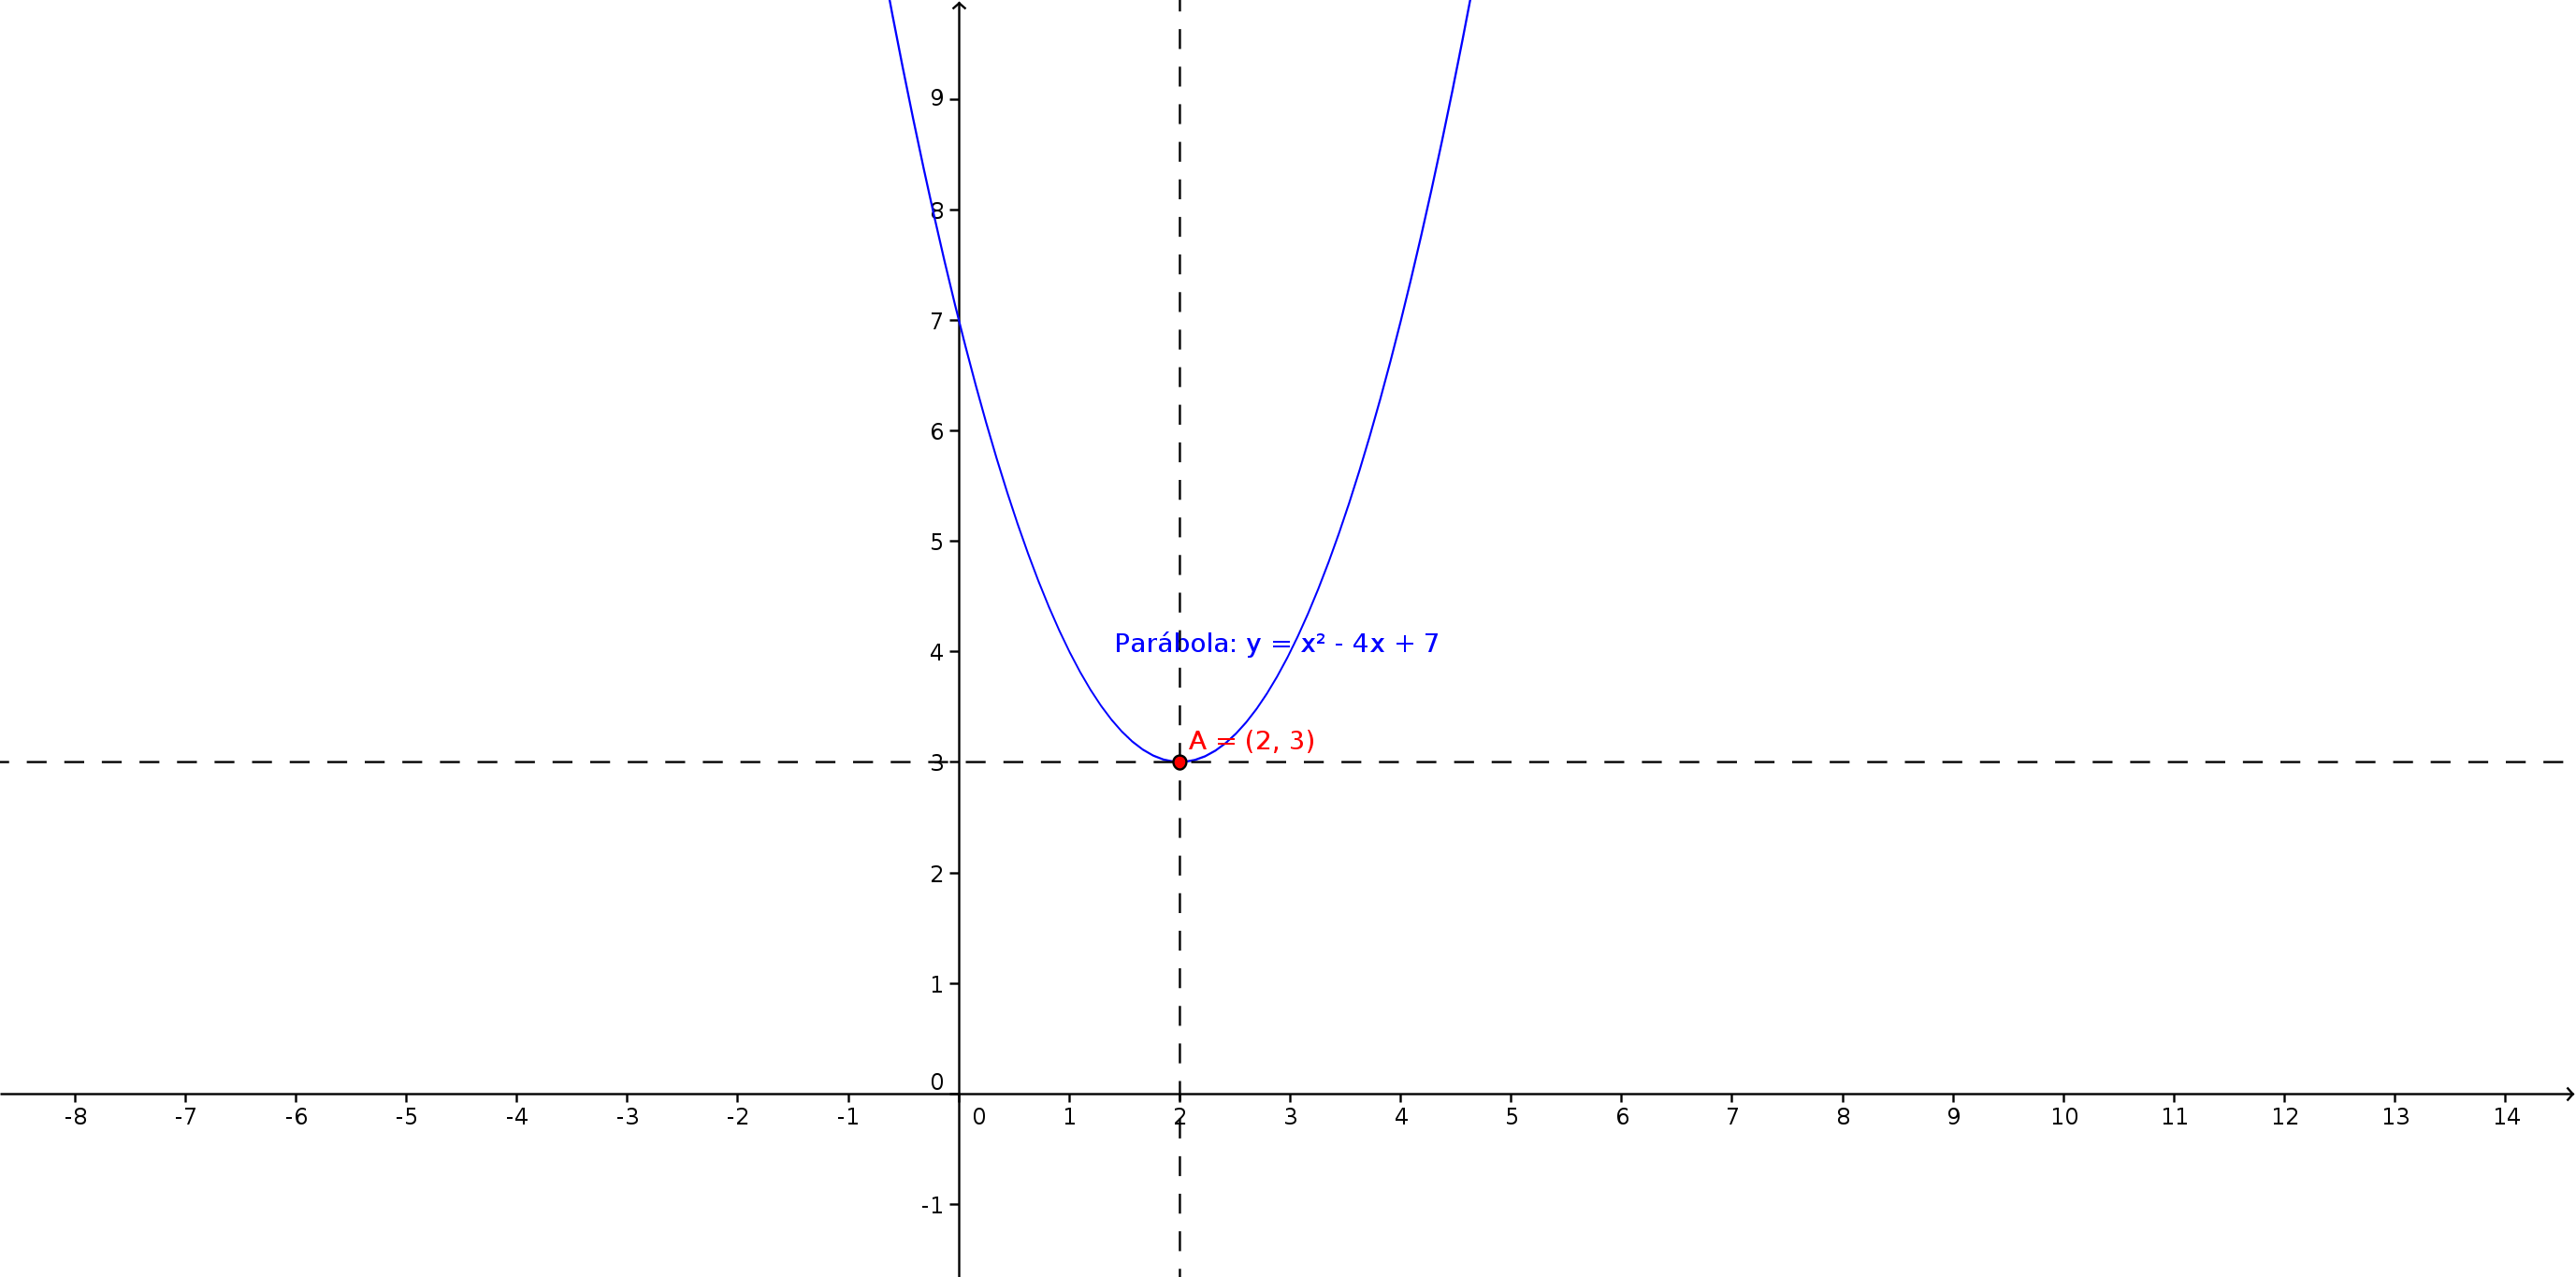
\includegraphics[height=5cm,keepaspectratio=true]{./precalculo/IM020401.png}
		% IM020401.png: 0x0 pixel, 300dpi, 0.00x0.00 cm, bb=
		\caption{$y=x^2-4x+7$}
		\label{fig:020401}
	\end{figure}
	


\subsection{Complemento de cuadrados}


	Cualquier funci\'on cuadrática se puede reescribir en la forma
	$$
	f(x)=a(x-h)^2+k,
	$$
	por el m\'etodo de \emph{complementos de cuadrado.}



	El punto $(h,k)$ se llama \emph{v\'ertice,} y corresponde al \emph{extremo} de la parábola
	$$
	y=a(x-h)^2+k.
	$$



	La f\'ormula para encontrar el v\'ertice de la parábola 
	$y=f(x)=ax^2+bx+c$ es
	$$\begin{cases}
		h=-\dfrac{b}{2a}\\
		k=f(h).
	\end{cases}
	$$ 



	Para completar el cuadrado, podemos usar el \emph{m\'etodo de divisi\'on sint\'etica:}
	\begin{center}
		\begin{tabular}{l|lll}
			$h$ & $a$ & $b$ & $c$\\
			& $\downarrow$ & $+ah$ & $\dots$\\\hline
			& $a$ & $\dots$ & $k$
		\end{tabular}
	\end{center}



	\begin{problema}
		Complete el cuadrado de
		$$y=x^2-4x+7.$$
	\end{problema}
	



	\begin{problema}
		Complete el cuadrádo de
		$$
		y=3x^2+30x+63.
		$$
	\end{problema}
	


\subsection{Intersecciones con los ejes}


	Las ra\'ices de un polinomio $p(x)$ son aquellos números reales $r$ tales que $p(r)=0.$



	Para encontrar las ra\'ices de una \emph{polinomio cuadrático}, necesitamos resolver la \emph{ecuaci\'on de segundo grado}
	$$
	a(x-h)^{2}+k=0.
	$$



	Si $r$ es una ra\'iz de $p(x)=a(x-h)^{2}+k,$ entonces la parábola $y=a(x-h)^{2}+k$ cruza al eje $x$ en el punto $(r,0).$




	\begin{observacion}
		Si bien $a,k>0$ o bien $a,k<0,$ entonces $a(x-h)^{2}+k>0$ y por tanto no existen ra\'ices. Por lo tanto, la parábola $y=a(x-h)^{2}+k$ \emph{nunca} cruza el eje $x.$ 
	\end{observacion}
	



	\begin{problema}
		Determine si existen ra\'ices de
		$$
		y=x^2-4x+7,
		$$ 
	\end{problema}
	



\subsection{Diferencia de cuadrados}


	Una identidad que es muy útil al momento de resolver ecuaciones es la \emph{diferencia de cuadrados}
	$$
	\left( a-b \right)\left( a+b \right)=a^{2}-b^{2}.
	$$



	Una ecuaci\'on de la forma 
	$$
	z^{2}-c^{2}=0
	$$
	se puede reescribir como
	$$
	\left( z-c \right)\left( z+c \right)=0...
	$$
	
	...en cuyo caso tenemos que $z-c=0$ o $z+c=0,$
	y por tanto las soluciones son
	$$
	z=\pm c.
	$$



	\begin{problema}
		Encuentre las ra\'ices de
		$$
		y=3x^2+30x+63.
		$$ 
	\end{problema}
	



	\begin{center}
		\includegraphics[height=5cm,keepaspectratio=true]{./precalculo/IM0301.png}
		% IM0301.png: 0x0 pixel, 300dpi, 0.00x0.00 cm, bb=
	\end{center}
	




\subsection{Ejemplos}


	\begin{problema} Resuelva las siguientes ecuaciones
		\begin{enumerate}
			\item $x^{2}-40=9$
			\item $2x^{2}-400=0$
			\item $x^{2}+36=9-2x^{2}$
		\end{enumerate}
		
	\end{problema}
	



	\begin{problema} Resuelva las siguientes ecuaciones
		\begin{enumerate}
			\item $\dfrac{x}{16}=\dfrac{4}{x}$
			\item $\dfrac{y^{2}}{3}=\dfrac{y^{2}}{6}+2$
		\end{enumerate}
		
	\end{problema}
	



	\begin{problema} Resuelva la siguiente ecuaci\'on
		$$
		\dfrac{1-2x}{3-x}=\dfrac{x-2}{3x-1}.
		$$
	\end{problema}
	



	\begin{problema} Resuelva la siguiente ecuaci\'on
		$$
		\dfrac{1}{2x-1}-\dfrac{1}{2x+1}=\dfrac{1}{4}.
		$$
	\end{problema}
	



	\begin{problema} Resuelva la siguiente ecuaci\'on
		$$
		x-\dfrac{2x}{x+1}=\dfrac{5}{x+1}-1.
		$$
	\end{problema}
	



	\begin{problema}
		\label{spi:exmp:16.2}
		Encuentre las ra\'ices de los siguientes polinomios
		\begin{enumerate}
			\item $7x^{2}-5x$
			\item $x^{2}-5x+6$
			\item $3x^{2}+2x-5$
			\item $x^{2}-4x+4$
		\end{enumerate}
		
	\end{problema}
	
	



	\begin{problema}
		\label{spi:exmp:16.3-}
		Encuentre las ra\'ices de los siguientes polinomios
		\begin{enumerate}
			\item $x^{2}-6x-2$
			\item $3x^2-5x+1$
			\item $4x^{2}-6x+3$   
		\end{enumerate}
		
	\end{problema}


\subsection{Factorizaci\'on}


	Si un polinomio $p(x)=ax^{2}+bx+c$ tiene ra\'ices $r_{1},r_{2}$ diferentes, entonces podemos factorizar de la siguiente manera
	$$
	p(x)=a(x-r_{1})\left( x-r_{2} \right).
	$$



	Si un polinomio $p(x)=ax^{2}+bx+c$ tiene una única ra\'z $r_{1}$, entonces podemos factorizar de la siguiente manera
	$$
	p(x)=a\left( x-r_{1} \right)^{2}.
	$$




	\begin{problema}
		\label{spi:exmp:16.2b}
		Factorice los siguientes polinomios
		\begin{enumerate}
			\item $7x^{2}-5x$
			\item $x^{2}-5x+6$
			\item $3x^{2}+2x-5$
			\item $x^{2}-4x+4$
		\end{enumerate}
		
	\end{problema}
	
	



	\begin{problema}
		\label{spi:exmp:16.3-b}
		Factorice los siguientes polinomios
		\begin{enumerate}
			\item $x^{2}-6x-2$
			\item $3x^2-5x+1$
			\item $4x^{2}-6x+3$   
		\end{enumerate}
		
	\end{problema}



\subsection{Aplicaciones}


	\begin{problema}
		\label{bron:exmp:16.21}
		Encuentre dos números positivos sabiendo que uno de ellos es igual al triple del otro más 5 y que el producto de ambos es igual a 68.
	\end{problema}
	



	\begin{problema}
		\label{bron:exmp:16.22}
		Encuentre un número sabiendo que la suma del triple del mismo con el doble de su rec\'iproco es igual a 5. 
	\end{problema}
	



	\begin{problema}
		\label{bron:exmp:16.23}
		Encuentre las dimensiones de un rectángulo cuto per\'imetro es de 50 pies y área es de 150 pies cuadrados. 
	\end{problema}



	\begin{problema}
		\label{bron:exmp:16.24}
		La hipotenusa de un triángulo es igual a 34 pulgadas. Encuentre las longitudes de los catetos sabiendo que uno de ellos es 14 pulgadas mayor que el otro.
	\end{problema}



	\begin{problema}
		\label{bron:exmp:16.25}
		Las dimensiones exteriores de un marco de fotograf\'ia son 12 por 15 pulgadas. Sabiendo que el ancho permanece constante, encuentre su valor a) cuando la superficie de la fotograf\'ia es de 88 pulgadas y b) cuando dicha superficie vale 100 pulgadas cuadradas. 
	\end{problema}



	\begin{problema}
		\label{bron:exmp:16.26}
		Un piloto realiza un vuelo de 600 millas. Sabiendo que si aumenta la velocidad en 40 millas/hora podr\'ia recorrer dicha distancia empleando 30 minutos menos, encuentre la velocidad promedio.  
	\end{problema}



	\begin{problema}
		\label{bron:exmp:16.27}
		Un comerciante compra determinado número de camisas por \$180 y las vende todas menos 6 con una ganancia de \$2 en cada camisa. Sabiendo que con el dinero recaudado en la venta podr\'ia haber comprado 30 camisas más que antes, calcule el precio de cada camisa.  
	\end{problema}



	\begin{problema}
		\label{bron:exmp:16.28}
		Dos operarios A y B juntos, realizan una tarea en 10 d\'ias. Trabajando por separado, A tardar\'ia 5 d\'ias más que B. Encuentre  el número de d\'ias que tardar\'ian en hacer la tarea trabajando cada no por s\'i s\'olo. 
	\end{problema}



\chapter{Trigonometría y Números complejos}


\section{La geometría de los triángulos: congruencia, similitud y el teorema de Pitágoras}

\subsection{Triángulos congruentes}

{}
	Los triángulos que tienen el mismo tamaño y la misma forma se llaman \emph{triángulos congruentes}.

{}
	\begin{center}
		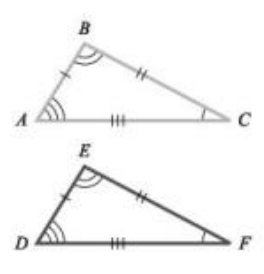
\includegraphics[height=8cm,keepaspectratio=true]{./trig/algsup3-01.png}
		% algsup3-01.png: 0x0 pixel, 300dpi, 0.00x0.00 cm, bb=
	\end{center}
	

{}
	Si dos triángulos $\triangle ABC, \triangle DEF$ son congruentes, escribiremos \begin{align*}
		\triangle ABC \cong \triangle DEF.
	\end{align*}

{}
	\begin{proposicion}[Criterios de congruencia]
		\begin{itemize}
			\item \emph{LAL}: Dos lados y su ángulo incluido iguales.
			\item \emph{ALA}: Dos ángulos y su lado incluido iguales. 
			\item \emph{LLL}: Tres lados iguales. 
		\end{itemize}
		
	\end{proposicion}
	


\subsection{Triángulos semejantes}
{}
	\begin{figure}
		%%%%%%%%%%%%%%%%%%%%%%%%%%%%%%%%%%%%%%%%%%%%%%%%%%%%%%%%%%%%%%%%%%%%%%%%%%%%%%%%%%%%%%%
		%%% You will need to add \usepackage{wrapfig} to your preamble to use textwrapping %%%
		%%%%%%%%%%%%%%%%%%%%%%%%%%%%%%%%%%%%%%%%%%%%%%%%%%%%%%%%%%%%%%%%%%%%%%%%%%%%%%%%%%%%%%%
		\centering
		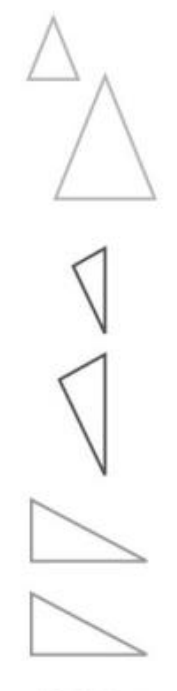
\includegraphics[width=2cm,keepaspectratio=true]{./trig/algsup3-02.png}
		% algsup3-02.png: 0x0 pixel, 300dpi, 0.00x0.00 cm, bb=
		\label{fig:3-02}
	\end{figure}
	
	Diremos que dos triángulos $\triangle ABC$ y $\triangle DEF$ son \emph{similares} si 
	existe un correspondencia $A\leftrightarrow D, B\leftrightarrow E, C \leftrightarrow F$
	tal que $\frac{|AB|}{|DE|}=\frac{|BC|}{|EF|}=\frac{|CA|}{|FD|}=: \alpha.$
	
	
	A tal \emph{constante de proporcionalidad} $\alpha$ se conoce como \emph{escala}.

{}
	\begin{proposicion}[Criterio \emph{AA}]
		Si las medidas de dos ángulos de un triángulo son iguales a las de dos ángulos correspondientes de un segundo triángulo, entonces los dos triángulos son semejantes.
	\end{proposicion}
	

{}
	\begin{problema}
		\label{exmp:9405}
		\begin{figure}
			%%%%%%%%%%%%%%%%%%%%%%%%%%%%%%%%%%%%%%%%%%%%%%%%%%%%%%%%%%%%%%%%%%%%%%%%%%%%%%%%%%%%%%%
			%%% You will need to add \usepackage{wrapfig} to your preamble to use textwrapping %%%
			%%%%%%%%%%%%%%%%%%%%%%%%%%%%%%%%%%%%%%%%%%%%%%%%%%%%%%%%%%%%%%%%%%%%%%%%%%%%%%%%%%%%%%%
			\centering
			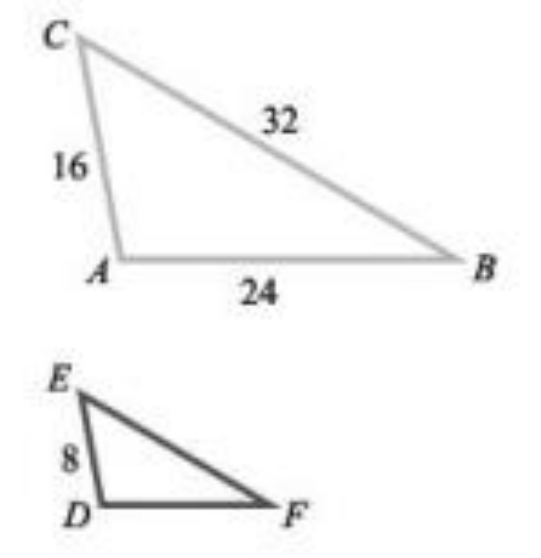
\includegraphics[width=5cm,keepaspectratio=true]{./trig/trig9446.png}
			% trig9446.png: 0x0 pixel, 300dpi, 0.00x0.00 cm, bb=
			\label{fig:9446}
		\end{figure}
		Suponga que en la figura, ambos triángulos son semejantes. Encuentre las longitudes desconocidas de los lados de $\triangle EDF.$
	\end{problema}
	

{}
	\begin{problema}
		\label{exmp:9406}
		\begin{figure}
			%%%%%%%%%%%%%%%%%%%%%%%%%%%%%%%%%%%%%%%%%%%%%%%%%%%%%%%%%%%%%%%%%%%%%%%%%%%%%%%%%%%%%%%
			%%% You will need to add \usepackage{wrapfig} to your preamble to use textwrapping %%%
			%%%%%%%%%%%%%%%%%%%%%%%%%%%%%%%%%%%%%%%%%%%%%%%%%%%%%%%%%%%%%%%%%%%%%%%%%%%%%%%%%%%%%%%
			\centering
			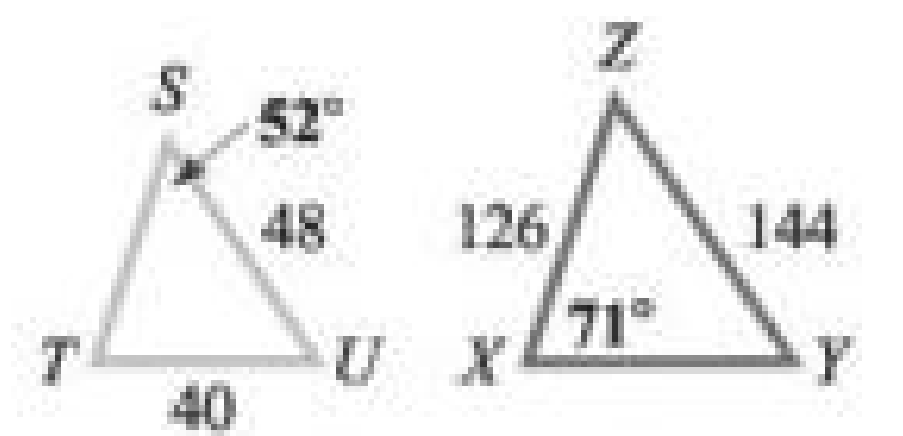
\includegraphics[width=5cm,keepaspectratio=true]{./trig/trig9447.png}
			% trig9446.png: 0x0 pixel, 300dpi, 0.00x0.00 cm, bb=
			\label{fig:9447}
		\end{figure}
		Encuentre las medidas de las partes desconocidas de los triángulos semejantes $\triangle STU$ y $\triangle ZXY.$ 
	\end{problema}
	

		\begin{figure}
	%%%%%%%%%%%%%%%%%%%%%%%%%%%%%%%%%%%%%%%%%%%%%%%%%%%%%%%%%%%%%%%%%%%%%%%%%%%%%%%%%%%%%%%
	%%% You will need to add \usepackage{wrapfig} to your preamble to use textwrapping %%%
	%%%%%%%%%%%%%%%%%%%%%%%%%%%%%%%%%%%%%%%%%%%%%%%%%%%%%%%%%%%%%%%%%%%%%%%%%%%%%%%%%%%%%%%
	\centering
	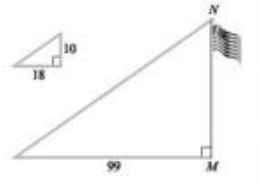
\includegraphics[width=5cm,keepaspectratio=true]{./trig/trig9448.png}
	% trig9446.png: 0x0 pixel, 300dpi, 0.00x0.00 cm, bb=
	\label{fig:9448}
\end{figure}

	\begin{problema}
		\label{exmp:9407}

		La jefa de oficina de correos de una ciudad quiere medir la altura del asta de la bandera de la oficina. Observa que en el instante en el que la sombra de la estación mide $18fts$, la sombra del asta mide $99fts$. El edificio tiene $10fts$ de altura. ¿Cuál es la altura del asta?
	\end{problema}
	

\subsection{El teorema de Pitágoras}
\begin{figure}
	%%%%%%%%%%%%%%%%%%%%%%%%%%%%%%%%%%%%%%%%%%%%%%%%%%%%%%%%%%%%%%%%%%%%%%%%%%%%%%%%%%%%%%%
	%%% You will need to add \usepackage{wrapfig} to your preamble to use textwrapping %%%
	%%%%%%%%%%%%%%%%%%%%%%%%%%%%%%%%%%%%%%%%%%%%%%%%%%%%%%%%%%%%%%%%%%%%%%%%%%%%%%%%%%%%%%%
	\centering
	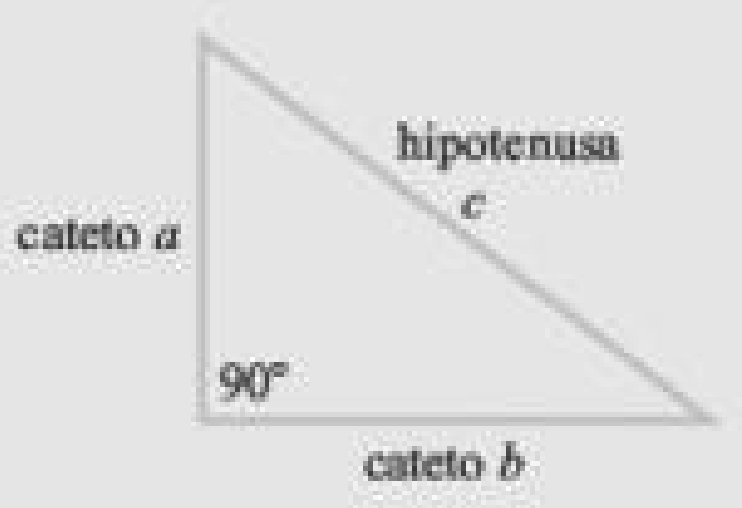
\includegraphics[width=5cm,keepaspectratio=true]{./trig/trig94thm.png}
	% trig94thm.png: 0x0 pixel, 300dpi, 0.00x0.00 cm, bb=
	\label{fig:94thm}
\end{figure}
{}
	\begin{teorema}[Pitágoras]
		\begin{align*}
			a^{2}+b^{2}=c^{2}
		\end{align*}
	\end{teorema}
	

{}
	Los números naturales $\set{3,4,5}$ forman una \emph{terna pitagórica}, ya que satisfacen las ecuaciones del teorema de Pitágoras. 

\begin{figure}
\centering
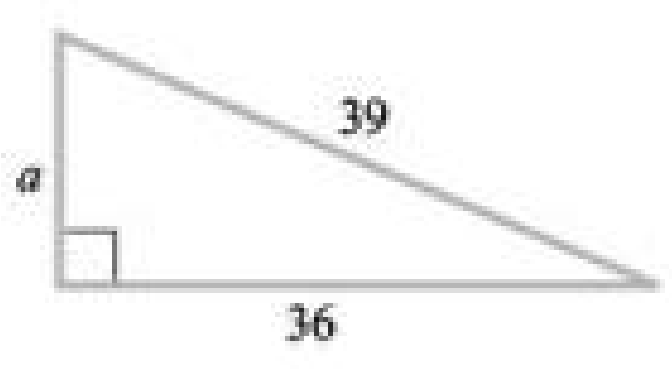
\includegraphics[width=5cm,keepaspectratio=true]{./trig/trig9450.png}
% trig9450.png: 0x0 pixel, 300dpi, 0.00x0.00 cm, bb=
\label{fig:9450}
\end{figure}

	\begin{problema}
		\label{exmp:9408}		
		Determine la longitud $a$ del triángulo rectángulo que se muestra.
	\end{problema}
	
\begin{figure}
\centering
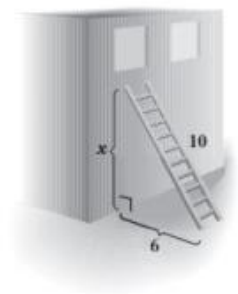
\includegraphics[width=5cm,keepaspectratio=true]{./trig/trig9451.png}
% trig9450.png: 0x0 pixel, 300dpi, 0.00x0.00 cm, bb=
\label{fig:9451}
\end{figure}

	\begin{problema}
		\label{exmp:9409}

		Una escalera de 10 metros de longitud tiene su base a 6 metros de la pared. ¿Qué altura alcanza la escalera?
	\end{problema}
	


\section{Los ángulos y sus medidas}
\subsection{Terminología básica}
{}
	\begin{figure}
		\centering
		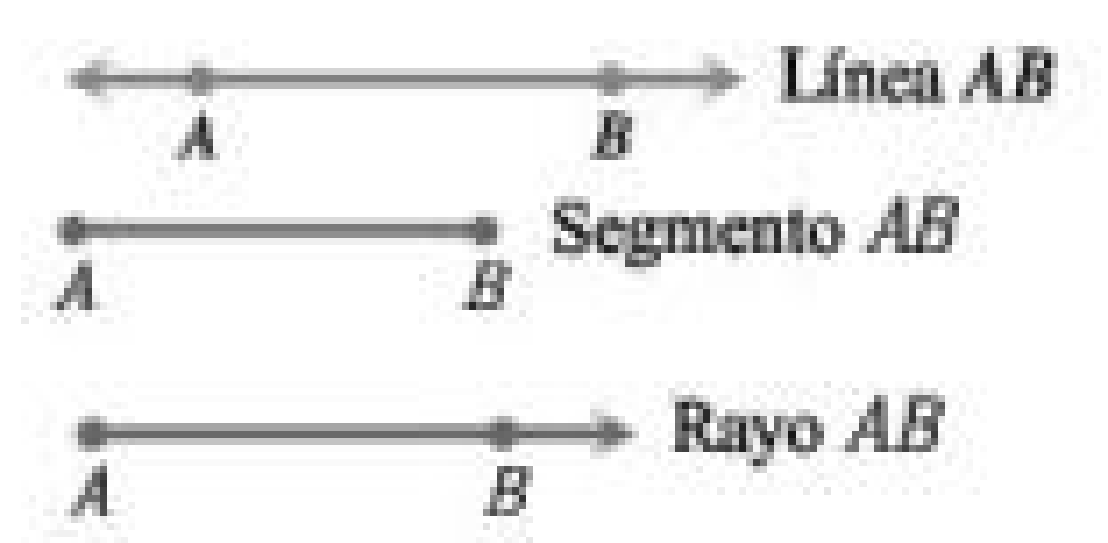
\includegraphics[width=10cm,keepaspectratio=true]{./trig/trig_101-1.png}
		% trig_10.1-1.png: 0x0 pixel, 300dpi, 0.00x0.00 cm, bb=
		\label{fig:101-1}
	\end{figure}
	

{}
	\begin{figure}
		\centering
		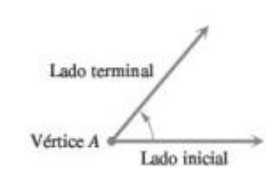
\includegraphics[width=10cm,keepaspectratio=true]{./trig/trig_101-2.png}
		% trig_10.1-1.png: 0x0 pixel, 300dpi, 0.00x0.00 cm, bb=
		\label{fig:101-2}
	\end{figure}
	

{}
	\begin{figure}
		\centering
		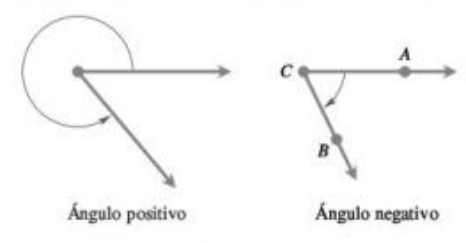
\includegraphics[width=10cm,keepaspectratio=true]{./trig/trig_101-3.png}
		% trig_10.1-1.png: 0x0 pixel, 300dpi, 0.00x0.00 cm, bb=
		\label{fig:101-3}
	\end{figure}
	

{}
	\begin{figure}
		\centering
		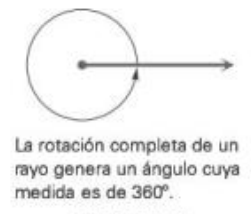
\includegraphics[width=10cm,keepaspectratio=true]{./trig/trig_101-4.png}
		% trig_10.1-1.png: 0x0 pixel, 300dpi, 0.00x0.00 cm, bb=
		\label{fig:101-4}
	\end{figure}
	

{}
	\begin{figure}
		\centering
		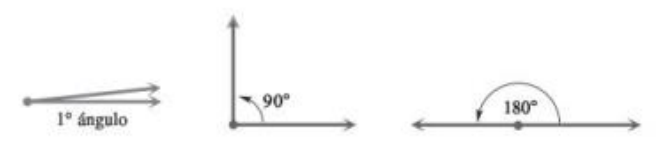
\includegraphics[width=10cm,keepaspectratio=true]{./trig/trig_101-5.png}
		% trig_10.1-1.png: 0x0 pixel, 300dpi, 0.00x0.00 cm, bb=
		\label{fig:101-5}
	\end{figure}
	

{}
	\begin{figure}
		\centering
		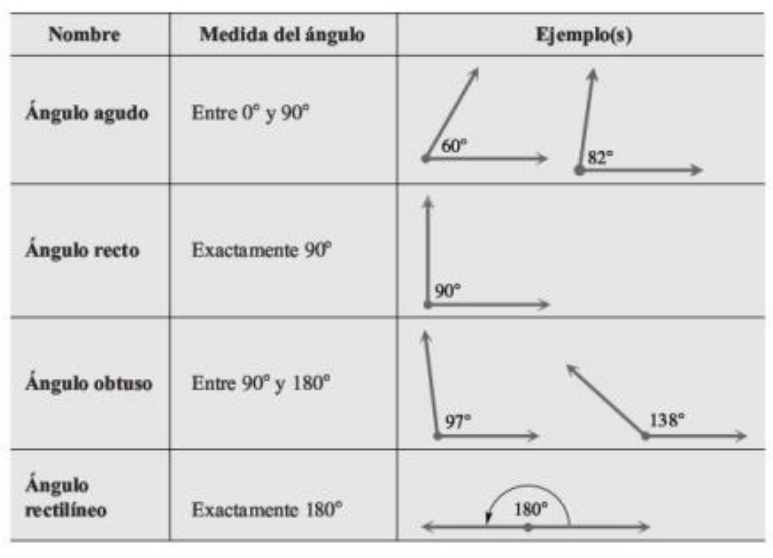
\includegraphics[width=8cm,keepaspectratio=true]{./trig/trig_101-tab1.png}
		% trig_101-tab1.png: 0x0 pixel, 300dpi, 0.00x0.00 cm, bb=
		\label{fig:101-tab1}
	\end{figure}
	

{}
	Si la suma de las medidas de  dos ángulos es $90^{o},$ los ángulos se llaman \emph{complementarios}. En tanto que dos ángulos cuyas medidas sumen $180^{o}$ son \emph{suplementarios}.

{}
	\begin{problema}
		\label{exmp:1011}
		Diga cuál es el complemento y el suplemento de $50^{o}$.
	\end{problema}
	

\subsection{Radianes}
{}
	Un \emph{ángulo central} es un ángulo positivo cuyo vértice esta en el centro de un círculo. 

{}
	\begin{figure}
		\centering
		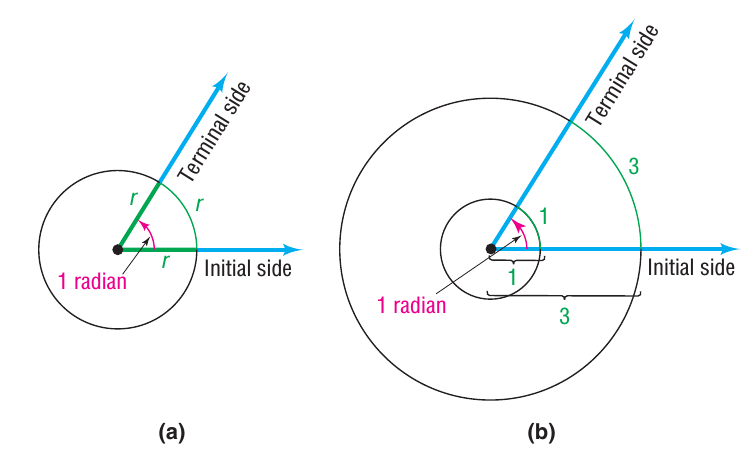
\includegraphics[height=5cm,keepaspectratio=true]{./trig/sull0610.png}
		% sull0610.png: 0x0 pixel, 300dpi, 0.00x0.00 cm, bb=
		\label{fig:sull6110}
	\end{figure}
	

{}
	\begin{teorema}[Longitud de arco]
		Para un círculo de radio $r$, un ángulo central  de $\theta$ radianes subtiende un arco cuya longitud es 
		\begin{align}
			\label{sull6104}
			s = r\theta
		\end{align}
	\end{teorema}
	

{}
	\begin{problema}
		\label{exmp:sull6103}
		Encuentre la longitud de arco de un círculo de radio $2$ subtendido por un ángulo central de $0.25$ radianes. 
	\end{problema}

{}
	\begin{problema}
		\label{exe:sull6171}
		Encuentre la longitud de arco de un círculo de radio $10$ subtendido por un ángulo central de $\frac{1}{2}$ radianes. 
	\end{problema}
	

\subsection{Conversión entre grados y radianes}
{}
	\begin{figure}
		\centering
		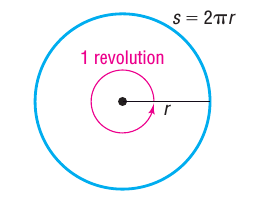
\includegraphics[height=5cm,keepaspectratio=true]{./trig/sull6112.png}
		% sull6112.png: 0x0 pixel, 300dpi, 0.00x0.00 cm, bb=
		\label{fig:sull6112}
		\caption{1 revolución = $2\pi$ radianes}
	\end{figure}
	

{}
	Como una revolución equivale a $360^{o},$ entonces $1 \texttt{rad}=360^{0}.$ De manera simplificada:
	\begin{align*}
		180^{o}= \pi\texttt{rad}
	\end{align*}

{}
	\begin{problema}
		Convierta cada uno de los ángulos a radianes:
		\begin{itemize}
			\item $60^{o}=$ 
			\item $150^{o}=$ 
			\item $-45^{o}=$ 
			\item $90^{o}=$ 
			\item $107^{o}$ 
		\end{itemize}
		
	\end{problema}
	

{}
	\begin{problema}
		\begin{itemize}
			\item Convierta $35^{o}$ a radianes, expresándolo como un múltiplo de $\pi$.
			\item Convierta $-40^{o}$ a radianes, expresándolo en decimales. 
		\end{itemize}
		
	\end{problema}
	

{}
	\begin{figure}
		\centering
		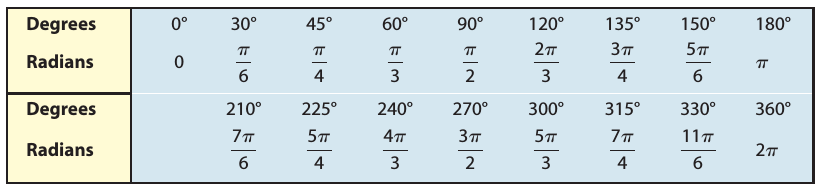
\includegraphics[width=10cm,keepaspectratio=true]{./trig/sull61t1.png}
		% sull61t1.png: 0x0 pixel, 300dpi, 0.00x0.00 cm, bb=
		\label{fig:61t1}
	\end{figure}
	

{}
	\begin{problema}
		La latitud de una locación $L$ es la medida del ángulo formado por un rayo dibujado desde el centro de la tierra al ecuador y un rayo dibujado del centro de la tierra a $L$. 
		
		Glasgow, Montana está al norte de Albuquerque, Nuevo México. Encuentre la distancia entre Glasgow, $48^{o}, 9'$, latitud Norte y Albuquerque, $35^{o}, 5'$. Suponga que el radio de la tierra es $3960$ millas.
	\end{problema}
	

{}
	\begin{figure}
		\centering
		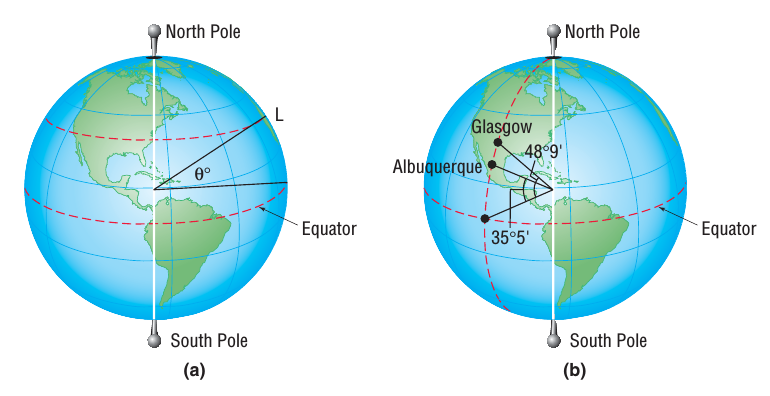
\includegraphics[width=10cm,keepaspectratio=true]{./trig/sull113.png}
		% sull113.png: 0x0 pixel, 300dpi, 0.00x0.00 cm, bb=
		\label{fig:sull6113}
	\end{figure}
	

{}
	\begin{problema}
		Memphis, Tennessee, está al norte de Nueva Orleans, Lousiana. Encuentre la distancia entre Memphis, $35^{o}, 9'$ latitud norte, y Nueva Orleans, $29^{o}, 57'$ latitud norte. Suponga que el radio de la tierra es $3960$ millas. 
	\end{problema}
	

\subsection{Área de un sector de un círculo} 
{}
	\begin{figure}
		\centering
		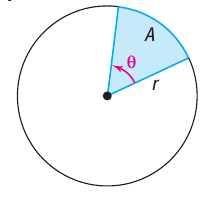
\includegraphics[height=5cm,keepaspectratio=true]{./trig/sull614.png}
		% sull614.png: 0x0 pixel, 300dpi, 0.00x0.00 cm, bb=
		\label{fig:sull6114}
	\end{figure}

{}
	\begin{figure}
		\centering
		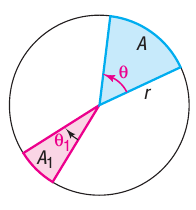
\includegraphics[height=5cm,keepaspectratio=true]{./trig/sull6115.png}
		% sull614.png: 0x0 pixel, 300dpi, 0.00x0.00 cm, bb=
		\label{fig:sull6115}
	\end{figure}

{}
	\begin{teorema}[Área de un sector]
		El área $A$ de un sector de un círculo de radio $r$ formado por un ángulo central de $\theta$ radianes es 
		\begin{align}
			\label{sull6108}
			A=\frac{1}{2}r^{2}\theta.
		\end{align}
	\end{teorema}
	

{}
	\begin{problema}
		\label{exmp:sull6107}
		Encuentre el área del sector de un círculo de radio $2fts$ formado por un ángulo de $30^{o}$. Redondee la respuesta dos decimales.  
	\end{problema}
	

{}
	\begin{problema}
		Encuentre el área del sector de un círculo de radio $10m$ formado por un ángulo de $\frac{1}{2}rad$. Redondee la respuesta dos decimales.  
	\end{problema}
	

\subsection{Movimiento circular}
{}
	\begin{figure}
		\centering
		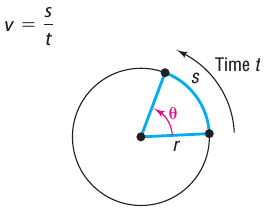
\includegraphics[height=5cm,keepaspectratio=true]{./trig/sull6116.png}
		% sull6116.png: 0x0 pixel, 300dpi, 0.00x0.00 cm, bb=
		\label{fig:sull6116}
	\end{figure}
	

{}
	Supongamos que un objeto se mueve alrededor de un círculo de radio $r$ a una rapidez constante. Si $s$ es la distancia recorrida en un tiempo $t$ alrededor del círculo, entonces la \emph{rapidez lineal} $v$ de este objeto se define como
	\begin{align}
		\label{sull6109}
		v=\dfrac{s}{t}
	\end{align}

{}
	La \emph{rapidez angular} $\omega$ de este objeto es el ángulo $\theta$ (medido en radianes) barrido, dividido por el lapso $t$, es decir, 
	\begin{align}
		\label{sull6110}
		\om=\dfrac{\theta}{t}.
	\end{align}
	
	De manera que 
	\begin{align}
		\label{sull6111}
		v = r\om.
	\end{align}

{}
	\begin{figure}{l}{6cm}
		%%%%%%%%%%%%%%%%%%%%%%%%%%%%%%%%%%%%%%%%%%%%%%%%%%%%%%%%%%%%%%%%%%%%%%%%%%%%%%%%%%%%%%%
		%%% You will need to add \usepackage{wrapfig} to your preamble to use textwrapping %%%
		%%%%%%%%%%%%%%%%%%%%%%%%%%%%%%%%%%%%%%%%%%%%%%%%%%%%%%%%%%%%%%%%%%%%%%%%%%%%%%%%%%%%%%%
		\centering
		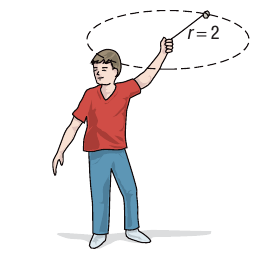
\includegraphics[width=5cm,keepaspectratio=true]{./trig/sull6117.png}
		% sull6117.png: 0x0 pixel, 300dpi, 0.00x0.00 cm, bb=
		\label{fig:6117}
	\end{figure}
	\begin{problema}
		\label{exmp:6108}
		Una persona está haciendo una roca atada al extremo de un cuerda de $2fts$ a un ritmo de $180rpm$. Encuentre la rapidez lineal de la roca en el instante en que es liberada.
	\end{problema}
	

{}
	\begin{problema}
		\label{exe:sull6197}
		Un objeto está viajando alrededor de un círculo de radio $5cm$. Si en $20s$ un ángulo central de $\dfrac{1}{3}rad$ es barrido, ¿cuál es su rapidez angular? ¿Cuál es su rapidez lineal?
	\end{problema}
	


	

\section{Funciones trigonométricas: El enfoque del círculo unitario}
\subsection{El círculo unitario}
{}
	\begin{figure}
		\centering
		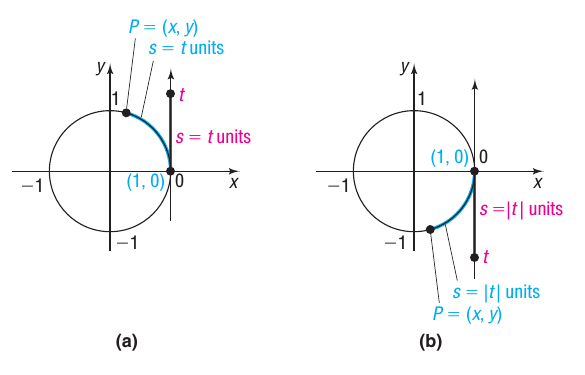
\includegraphics[width=10cm,keepaspectratio=true]{./trig/sull0618.png}
		% sull0618.png: 0x0 pixel, 300dpi, 0.00x0.00 cm, bb=
		\label{fig:0618}
	\end{figure}
	

{}
	\begin{definicion}[Funciones trigonométricas]
		Sea $t$ un número real y $P=(x,y)$ el punto en el círculo unitario que corresponde a $t$.
		\begin{multicols}{2}
			\begin{itemize}
				\item $\sin(t)=y$
				\item $\cos(t)=x$
				\item $\tan(t)=\frac{y}{x}$
				\item $\csc(t)=\frac{1}{y}$
				\item $\sec(t)=\frac{1}{x}$
				\item $\cot(t)=\frac{x}{y}$
			\end{itemize}
		\end{multicols}
	\end{definicion}

{}
	\begin{problema}
		\label{exmp:sull0601}
		Sea $t$ un número real y $P=\left(-\dfrac{1}{2}, \dfrac{\sqrt{3}}{2}  \right)$
		un punto en el círculo unitario que corresponde a $t$.  Encuentre los valores de las seis funciones trigonométricas.
	\end{problema}
	

{}
	\begin{figure}
		\centering
		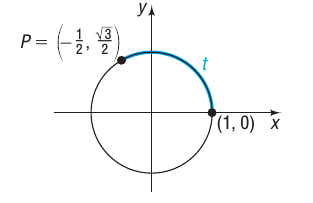
\includegraphics[width=10cm,keepaspectratio=true]{./trig/sull0619.png}
		% sull0618.png: 0x0 pixel, 300dpi, 0.00x0.00 cm, bb=
		\label{fig:0619}
	\end{figure}

{}
	\begin{problema}
		Sea $t$ un número real y $P=\left(\dfrac{\sqrt{3}}{2}, \dfrac{1}{2} \right)$
		un punto en el círculo unitario que corresponde a $t$. Encuentre los valores de las seis funciones trigonométricas.
	\end{problema}
	

\subsection{Funciones trigonométricas de ángulos}
{}
	\begin{figure}
		\centering
		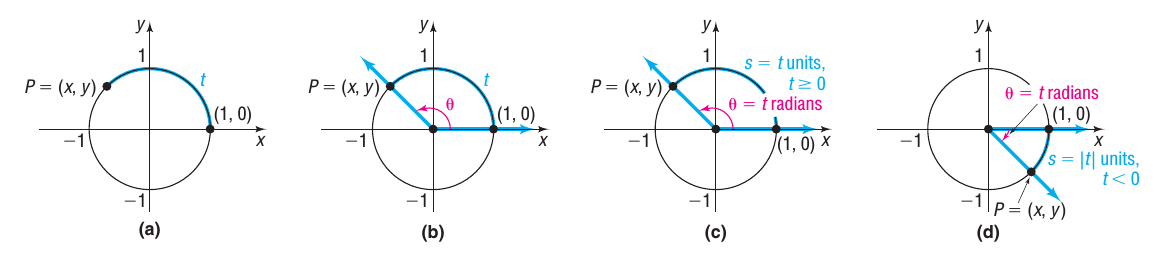
\includegraphics[width=10cm,keepaspectratio=true]{./trig/sull0620.png}
		% sull0618.png: 0x0 pixel, 300dpi, 0.00x0.00 cm, bb=
		\label{fig:0620}
	\end{figure}

{}
	Entonces, podemos definir una función trigonométrica en ángulos siempre y cuando este medido en radianes:
	\begin{align*}
		f(\theta)=f(t \texttt{ radianes})
	\end{align*} si $\theta= t \texttt{ radianes}$.

{}
	\begin{problema}
		\label{exmp:sull0602}
		Encuentre el valor exacto de las seis funciones trigonométricas en:
		\begin{itemize}
			\item $\theta=0=0^{o}$
			\item $\theta=\frac{\pi}{2}=90^{o}$ 
			\item $\theta=\pi=180^{o}$ 
			\item $\theta=\frac{3\pi}{2}=270^{o}$
		\end{itemize}
		
	\end{problema}
	

{}
	\begin{figure}
		\centering
		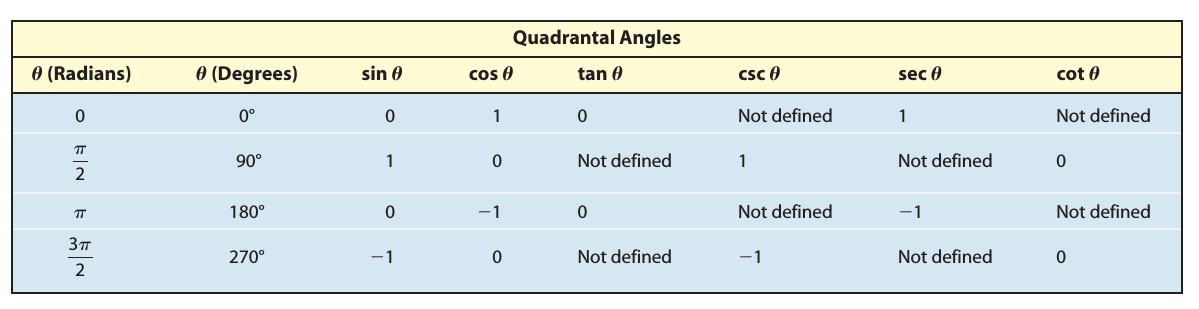
\includegraphics[width=11cm,keepaspectratio=true]{./trig/sull06t2.png}
		% sull06t2.png: 0x0 pixel, 300dpi, 0.00x0.00 cm, bb=
		\label{fig:06t2}
	\end{figure}
	

{}
	\begin{problema}
		\label{exmp:sull0603}
		Encuentre el valor exacto de:
		\begin{itemize}
			\item $\sin(3\pi)$ 
			\item $\cos(-270^{o})$
		\end{itemize}
	\end{problema}
	

{}
	\begin{problema}
		\label{exmp:sull0604}
		Encuentre el valor exacto de las seis funciones trigonométricas en $\frac{\pi}{4}=45^{o}$.
	\end{problema}
	

{Valor exacto en $\frac{\pi}{4}$}
	\begin{problema}
		\label{exmp:sull0605}
		Encuentre el valor exacto de cada expresión:
		\begin{itemize}
			\item $\sin(45^{o})\cos(180^{o})$
			\item $\tan\left( \frac{\pi}{4} \right)-\sin\left( \frac{3\pi}{2} \right)$
			\item $\left( \sec\frac{\pi}{4} \right)^{2}+\csc\frac{\pi}{2}$
		\end{itemize}
		
	\end{problema}
	

{Valor exacto en $\frac{\pi}{6}$ y $\frac{\pi}{3}$}
	\begin{figure}
		\centering
		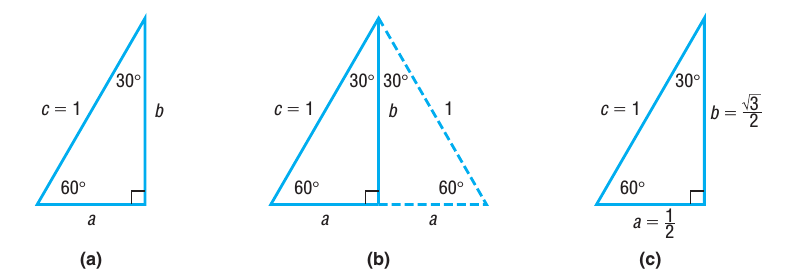
\includegraphics[width=10cm,keepaspectratio=true]{./trig/sull0624.png}
		% sull0624.png: 0x0 pixel, 300dpi, 0.00x0.00 cm, bb=
		\label{fig:0624}
	\end{figure}
	

{}
	\begin{problema}
		\label{exmp:0606}
		Encuentre el valor exacto de las seis funciones trigonométricas de $\frac{\pi}{3}=60^{o}$.
	\end{problema}
	

{}
	\begin{problema}
		\label{exmp:0607}
		Encuentre el valor exacto de las seis funciones trigonométricas de $\frac{\pi}{6}=30^{o}$.
	\end{problema}
	

{}
	\begin{figure}
		\centering
		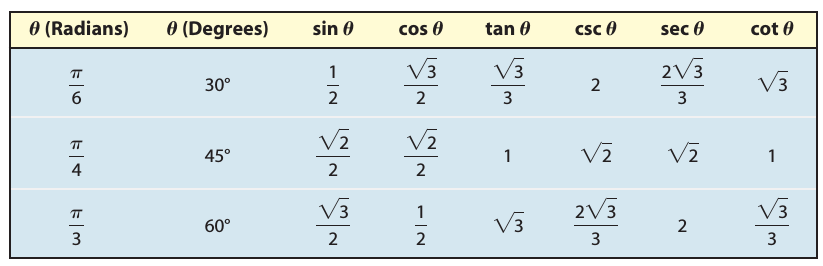
\includegraphics[width=11cm,keepaspectratio=true]{./trig/sull06t3.png}
		% sull06t3.png: 0x0 pixel, 300dpi, 0.00x0.00 cm, bb=
		\label{fig:tab3}
	\end{figure}
	

{}
	\begin{problema}
		Un recolector de lluvia se construye a partir de planchas de aluminio de 12 pulgadas de ancho. Después de marcar 4 pulgadas a partir de cada extremo, está longitud se dobla a un ángulo $\theta$. Encuentre el área transversal máxima del recolector. 
	\end{problema}


	\begin{figure}
		\centering
		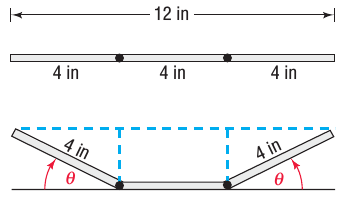
\includegraphics[width=10cm,keepaspectratio=true]{./trig/sull0627.png}
		% sull0627.png: 0x0 pixel, 300dpi, 0.00x0.00 cm, bb=
		\label{fig:0627}
	\end{figure}



\section{Funciones trigonométricas inversas}

\subsection{Funciones inversas}
{}
	Sea $f:A\to B$ una función. Diremos que $f$ es \emph{invertible} si para cada $y\in B$ \emph{siempre} corresponde un \emph{único} $x\in A$, tal que
	\begin{align*}
		f(x)=y.
	\end{align*}

{}
	Si una función $f$ es invertible, entonces existe una función $g:B\to A$ tal que $y=f(x)$ si y solo si $g(y)=x$.  En otras palabras, podemos despejar $x$.  Es usual denotar a tal función $g$ por $f^{-1}$ y llamarle \emph{inversa de $f$}.

{Propiedades del inversa}
	\begin{itemize}
		\item $f^{-1}\left( f(p) \right)$ para todo $p\in A.$ 
		\item $f\left( f^{-1}(p) \right)$ para todo $p\in B.$ 
		\item $\texttt{Dominio}(f)=\texttt{Rango}(f^{-1})$ y viceversa. 
		\item La gráfica de $f^{-1}$ es la reflexión a $45^{o}$ de la gráfica de $f$.
	\end{itemize}
	

% \subsection{Seno inverso}
% {}
% \begin{figure}
%  \centering
%  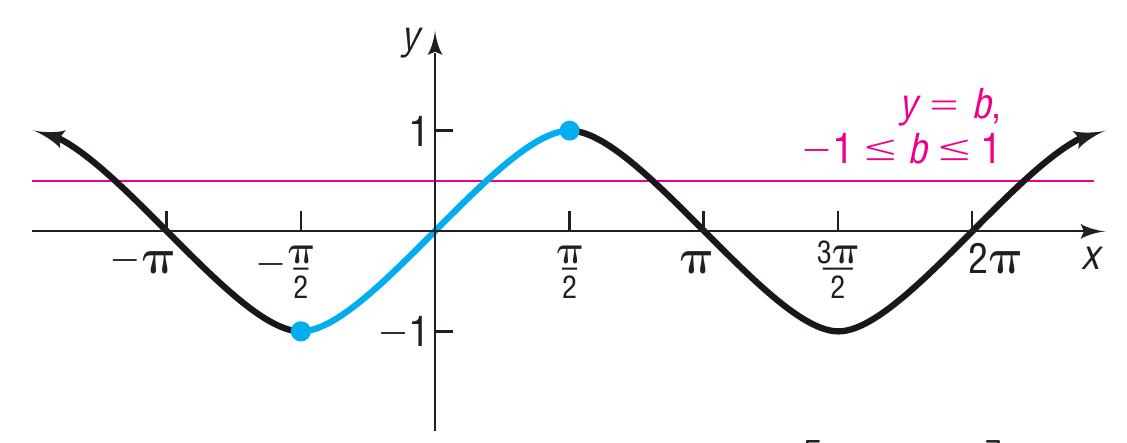
\includegraphics[width=11cm,keepaspectratio=true]{./trig/sull0701.png}
%  % sull0701.png: 0x0 pixel, 300dpi, 0.00x0.00 cm, bb=
%  \label{fig:0701}
%  \caption{$y=\sin(x), -\infty<x<\infty, -1\leq y \leq 1$}
% \end{figure}
% 
% 
% {}
% \begin{figure}
%  \centering
%  \includegraphics[height=7cm,keepaspectratio=true]{./trig/sull0702.png}
%  % sull0702.png: 0x0 pixel, 300dpi, 0.00x0.00 cm, bb=
%  \caption{$y=\sin(x), -\frac{\pi}{2}\leq x \leq \frac{\pi}{2}, -1\leq y \leq 1$}
%  \label{fig:0702}
% \end{figure}
% 
% 
% {}
% \begin{figure}
%  \centering
%  \includegraphics[height=6cm,keepaspectratio=true]{./trig/sull0703.png}
%  % sull0703.png: 0x0 pixel, 300dpi, 0.00x0.00 cm, bb=
%  \caption{$y=\sin^{-1}x, -1\leq x \leq 1, -\dfrac{\pi}{2}\leq y \leq \dfrac{\pi}{2}$}
%  \label{fig:0703}
% \end{figure}
% 
% 
% {Seno inverso}
% $$
% y = \sin^{-1} \iff
% \begin{cases}
%  x=\sin(y)\\
%  -1 \leq x \leq 1 \\
%  -\dfrac{\pi}{2} \leq y \leq \dfrac{\pi}{2}
% \end{cases}
% $$
% 
% {}
% \begin{problema}
%  Encuentre el valor exacto de
%  \begin{itemize}
%   \item $\sin^{-1}(1)$ 
%   \item $\sin^{-1}(0)$ 
%   \item $\sin^{-1}\left( -\frac{1}{2} \right)$ 
%   \item $\sin^{-1}\left( \frac{\sqrt{2}}{2} \right)$
%  \end{itemize}
% 
% \end{problema}
% 
% 
% {}
% \begin{problema}
%  Encuentre el valor exacto de 
%  \begin{itemize}
%   \item $\sin^{-1}\left( \sin\left( \frac{\pi}{8} \right) \right)$
%   \item $\sin^{-1}\left( \sin\left( \frac{5\pi}{8} \right) \right)$
%  \end{itemize}
% 
% \end{problema}
% 
% 
% {}
% \begin{problema}
%  Encuentre el valor exacto de 
%  \begin{itemize}
%   \item $\sin\left( \sin^{-1}(0.5) \right)$ 
%   \item $\sin\left( \sin^{-1}(1.8) \right)$ 
%   \item $\sin\left( \sin^{-1}\left( \frac{1}{4} \right) \right)$
%  \end{itemize}
% 
% \end{problema}
% 
% 

% \subsection{Coseno inverso}
% {}
% \begin{figure}
%  \centering
%  \includegraphics[width=10cm,keepaspectratio=true]{./trig/sull0707.png}
%  % sull0707.png: 0x0 pixel, 300dpi, 0.00x0.00 cm, bb=
%  \caption{$y=\cos(x),-\infty < x <\infty, -1\leq y \leq 1$}
%  \label{fig:0707}
% \end{figure}
% 
% 
% {}
% \begin{figure}
%  \centering
%  \includegraphics[width=10cm,keepaspectratio=true]{./trig/sull0708.png}
%  % sull0708.png: 0x0 pixel, 300dpi, 0.00x0.00 cm, bb=
%  \caption{$y=\cos(x),0 \leq x \leq \pi, -1\leq y \leq 1$}
%  \label{fig:0708}
% \end{figure}
% 
% 
% {}
% \begin{figure}
%  \centering
%  \includegraphics[width=7cm,keepaspectratio=true]{./trig/sull0709.png}
%  % sull0709.png: 0x0 pixel, 300dpi, 0.00x0.00 cm, bb=
%  \caption{$y=\cos(x), -1\leq x \leq 1, 0\leq y \leq \pi$}
%  \label{fig:0709}
% \end{figure}
% 
% 
% {Coseno inverso}
% $$y=\cos^{-1}(x)\iff
% \begin{cases}
%  x=\cos(y) \\
%  -1\leq x \leq 1 \\
%  0 \leq y \leq \pi
% \end{cases}
% $$
% 
% {}
% \begin{problema} Encuentre el valor exacto de
%  \begin{itemize}
%   \item $\cos^{-1}(0)$ 
%   \item $\cos^{-1}\left( -\frac{\sqrt{2}}{2} \right)$
%  \end{itemize}
% 
% \end{problema}
% 
% 
% {}
% \begin{problema}
%  Encuentre el valor exacto de:
%  \begin{itemize}
%   \item $\cos^{1}\left( \cos\frac{\pi}{12} \right)$
%   \item $\cos\left( \cos^{-1}(-0.4) \right)$ 
%   \item $\cos^{-1}\left( \cos\left( -\frac{2\pi}{3} \right) \right)$ 
%   \item $\cos\left( \cos^{-1}\pi \right)$
%  \end{itemize}
% 
% \end{problema}
% 
% 

\subsection{Tangente inversa}
{}
	\begin{figure}
		\centering
		\includegraphics[width=10cm,keepaspectratio=true]{./trig/sull0712.png}
		% sull0712.png: 0x0 pixel, 300dpi, 0.00x0.00 cm, bb=
		\label{fig:0712}
		\caption{$y=\tan(x)$}
	\end{figure}
	

{}
	\begin{figure}
		\centering
		\includegraphics[height=7cm,keepaspectratio=true]{./trig/sull0713.png}
		% sull0713.png: 0x0 pixel, 300dpi, 0.00x0.00 cm, bb=
		\caption{$y=\tan(x), \; -\frac{\pi}{2}<x<\frac{\pi}{2}, \; 
			-\infty < x < \infty$}
		\label{fig:0713}
	\end{figure}
	

{}
	\begin{figure}
		\centering
		\includegraphics[height=7cm,keepaspectratio=true]{./trig/sull0714.png}
		% sull0714.png: 0x0 pixel, 300dpi, 0.00x0.00 cm, bb=
		\label{fig:0714}
	\end{figure}
	

{}
	\begin{figure}
		\centering
		\includegraphics[width=10cm,keepaspectratio=true]{./trig/arctan.png}
		% arctan.png: 0x0 pixel, 300dpi, 0.00x0.00 cm, bb=
		\caption{$y=\tan^{-1}(x)$}
		\label{fig:arctan}
	\end{figure}

{Tangente inversa}
	$$y=\tan^{-1}(x)\iff
	\begin{cases}
		x=\tan(y)\\
		-\infty < x < \infty \\
		-\dfrac{\pi}{2} < y < \dfrac{\pi}{2}
	\end{cases}
	$$


{}
	\begin{problema}
		Encuentre el valor exacto de
		\begin{itemize}
			\item $\tan^{-1} 1$ 
			\item $\tan(-\sqrt{3})$ 
			\item $\tan^{-1}0$ 
			\item $\tan^{-1}\left( \tan\frac{4\pi}{5} \right)$
		\end{itemize}
		
	\end{problema}


\subsection{Vectores}
{}
	Diremos que un vector $\langle x,y \rangle$ esta en su \emph{forma polar (estándar)} ${\color{red}r\exp(\theta i)}$ si 
	\begin{align*}
		x =& r\cos(\theta)\\
		y =& r\sin(\theta)
	\end{align*} con $-\pi < \theta \leq \pi$.

{}
	\begin{center}
		\includegraphics[height=5cm,keepaspectratio=true]{./trig/Examples_of_Polar_Coordinates.png}
		% Examples_of_Polar_Coordinates.svg.png: 0x0 pixel, 300dpi, 0.00x0.00 cm, bb=
	\end{center}
	

{}
	\begin{problema}
		Escriba los siguientes vectores en su forma polar (estándar):
		\begin{itemize}
			\item $\langle 1, \sqrt{3}\rangle$ 
			\item $\langle 1, -\sqrt{3}\rangle$ 
			\item $\langle -1, \sqrt{3}\rangle$ 
			\item $\langle -1, -\sqrt{3}\rangle$ 
		\end{itemize}
		
	\end{problema}
	

\subsection{Optimización}

	\begin{problema}
		\label{exe:0776}
		Suponga que en una sala de cine, una pantalla tiene 28 pies de alto. Cuando un espectador se sienta, la parte inferior de la pantalla tiene una altura de 6 pies por encima de su nivel de visión. El ángulo formado al dibujar una linea desde la parte inferior de la pantalla a la parte superior se conoce como ángulo de visión. Encuentre el ángulo máximo de visión respecto a la distancia al muro que sostiene la pantalla.
	\end{problema}


{}
	\begin{figure}
		\centering
		\includegraphics[width=10cm]{./trig/angulo_vision.png}
		% angulo_vision.png: 0x0 pixel, 300dpi, 0.00x0.00 cm, bb=
		\caption{Ángulo de visión}
		\label{fig:angulo_vision}
	\end{figure}
	

{Sugerencia}
	\begin{align*}
		\dfrac{d}{dx}\left( \tan^{-1}\left( \dfrac{A}{x} \right) \right)=
		-\dfrac{A}{A^{2}+x^{2}}
	\end{align*}



\section{Propiedades de funciones trigonométricas}

{}
	\begin{problema}
		\begin{itemize}
			\item Grafique cada una de las seis funciones trigonométricas en \texttt{Sagemath}.
			\item Determine el dominio y el rango de cada una.
		\end{itemize}  
	\end{problema}
	

{}
	\begin{definicion}
		Una función se llama periódica si existe un número positivo $p$ tal que siempre que $\theta$ esté en el dominio de $f,$ entonces $\theta+p$ lo está y 
		\begin{align*}
			f(\theta+p)=f(\theta).
		\end{align*}
		
		Si existe un número minimal $p$ con tal propiedad, diremos que este es el \emph{periodo fundamental} de $f.$
	\end{definicion}

{}
	\begin{problema}
		Determine el periodo respectivo de cada una de las seis funciones trigonométricas.
	\end{problema}
	


	\begin{problema}
		\label{exmp:6301}
		Encuentre el valor exacto de 
		\begin{itemize}
			\item $\sin\left( \dfrac{17\pi}{4} \right)$
			\item $\cos\left( 5\pi \right)$
			\item $\tan\left( \dfrac{5\pi}{4} \right)$
		\end{itemize}
		
	\end{problema}

{}
	\begin{figure}
		\centering
		\includegraphics[width=11cm,keepaspectratio=true]{./trig/sull0628.png}
		% sull0628.png: 0x0 pixel, 300dpi, 0.00x0.00 cm, bb=
		\label{fig:0638}
	\end{figure}
	

{}
	\begin{problema}
		Determine el valor exacto de 
		\begin{itemize}
			\item $\sin(405^{o})$
			\item $\cot(390^{o})$
			\item $\sec\left( \dfrac{17\pi}{4} \right)$
		\end{itemize}
		
	\end{problema}
	

{Identidades reciprocas}
	\begin{align}
		\label{sull632}
		\csc(\theta)&= \dfrac{1}{\sin(\theta)}\\
		\sec(\theta)&= \dfrac{1}{\cos(\theta)}\\
		\cot(\theta)&= \dfrac{1}{\tan(\theta)}
	\end{align}

{}
	\begin{problema}
		\label{exmp:6303}
		Dado 
		\begin{align*}
			\sin(\theta)&= \dfrac{\sqrt{5}}{5}\\
			\cos(\theta)&= \dfrac{2\sqrt{5}}{5}
		\end{align*}
		encuentre el valor de las cuatro funciones trigonométricas restantes.
	\end{problema}
	

{}
	\begin{problema}
		\label{exe:6335}
		Dado 
		\begin{align*}
			\sin(\theta)&= -\dfrac{3}{5}\\
			\cos(\theta)&= \dfrac{4}{5}
		\end{align*}
		encuentre el valor de las cuatro funciones trigonométricas restantes.
	\end{problema}
	

{Identidades pitagóricas}
	\begin{align*}
		\sin^{2}\theta+\cos^{2}\theta=1
	\end{align*} 
	\begin{align*}
		\tan^{2}\theta + 1 = \sec^{2}\theta
	\end{align*} 
	\begin{align*}
		\cot^{2}\theta + 1 =\csc^{2}\theta
	\end{align*}


	La función coseno es par:
	$$ \cos(-x)=\cos(x) $$
	mientras que la función seno es impar:
	$$ \sin(-x)=-\sin(x) .$$

{}
	\begin{problema}
		\label{exmp:6304}
		Encuentre el valor exacto de cada expresión \emph{sin usar calculadora}:
		\begin{itemize}
			\item $\tan(20^{o})-\dfrac{\sin(20^{o})}{\cos(20^{o})}$ 
			\item $\sin^{2}\dfrac{\pi}{12}+\dfrac{1}{\sec^{2}\dfrac{\pi}{12}}$
		\end{itemize}
		
	\end{problema}
	

{}
	\begin{problema}
		Encuentre el valor exacto de cada expresión \emph{sin usar la calculadora}:
		\begin{itemize}
			\item $\sin(80^{o})\csc(80^{o})$
			\item $\cos(400^{o})\sec(40^{o})$
			\item $\dfrac{\sin(-20^{o})}{\cos(380^{o})}+\tan(200^{o})$
		\end{itemize}
		
	\end{problema}
	


	\begin{problema}
		\label{exmp:sull6305}
		Dado que $\sin\theta=\frac{1}{3}$ y $\cos\theta$, encuentre el valor exacto de cada una de las restantes cinco funciones trigonométricas.
	\end{problema}
	

{}
	\begin{figure}
		\centering
		\includegraphics[height=8cm]{./trig/sull0641.png}
		% sull0641.png: 0x0 pixel, 300dpi, 0.00x0.00 cm, bb=
		\label{fig:0641}
	\end{figure}
	

{}
	

{}
	\begin{problema}
		Dado que $\tan\theta=\dfrac{1}{2}$ y $\sin\theta<0$, encuentre el valor exacto de cada una de las restantes cinco funciones trigonométricas en $\theta$.
	\end{problema}
	

{}
	\begin{figure}
		\centering
		\includegraphics[height=8cm]{./trig/sull0642.png}
		% sull0641.png: 0x0 pixel, 300dpi, 0.00x0.00 cm, bb=
		\label{fig:0642}
	\end{figure}
	

{}
	\begin{problema}
		Encuentre el valor de cada una de las restantes funciones trigonométricas en $\theta$ conociendo que $\sin\theta=\dfrac{12}{13}$ y $\theta$ se encuentra en el segundo cuadrante.
	\end{problema}
	

{Paridad e imparidad}
	Por un lado, una función $f(\theta)$ es par si $f(-\theta)=f(\theta).$  Por otro lado, función $f(\theta)$ si $f(-\theta)=-f(\theta).$

{}
	\begin{figure}
		\centering
		\includegraphics[height=8cm,keepaspectratio=true]{./trig/sull0443.png}
		% sull0443.png: 0x0 pixel, 300dpi, 0.00x0.00 cm, bb=
		\label{fig:0643}
	\end{figure}
	


	\begin{proposicion}
		La función $\cos$ es par, pero la función $\sin$ es par. 
	\end{proposicion}
	

{}
	\begin{problema}
		Determine si las funciones trigonométricas restantes son pares o impares.
	\end{problema}
	

{}
	\begin{problema}
		\label{exmp:0607}
		Encuentre el valor exacto de 
		\begin{itemize}
			\item $\sin(-45^{o})$ 
			\item $\cos(-\pi)$ 
			\item $\cot\left( -\dfrac{3\pi}{2} \right)$ 
			\item $\tan\left( -\dfrac{37\pi}{4} \right)$
		\end{itemize}
		
	\end{problema}
	

{}
	\begin{problema}
		\begin{itemize}
			\item $\sin(-60^{o})$
			\item $\csc(-30^{o})$
			\item $\cos\left( -\dfrac{\pi}{4} \right)$
			\item $\sec(-\pi)$
		\end{itemize}
		
	\end{problema}


\section{Suma y diferencias de ángulos}

{Suma y diferencias para el coseno}
	\begin{align*}
		\cos(s+t) &= \cos(s)\cos(t)-\sin(s)\sin(t) \\  
		\cos(s-t) &= \cos(s)\cos(t)+\sin(s)\sin(t)
	\end{align*}



	\begin{problema} Demuestre las siguientes identidades
		\begin{align*}
			\cos\left(\dfrac{\pi}{2}-t\right) &= \sin(t) \\
			\sin\left(\dfrac{\pi}{2}-t\right) &= \cos(t) 
		\end{align*}
	\end{problema}


{Suma y diferencias para el coseno}
	\begin{align*}
		\sin(s+t) &= \sin(s)\cos(t)+\cos(s)\sin(t) \\  
		\sin(s-t) &= \sin(s)\cos(t)-\cos(s)\sin(t)
	\end{align*}



	\begin{problema}
		Establezca la siguiente identidad
		\begin{align*}
			\dfrac{\cos\left(s-t\right)}{\sin(s)\sin(t)} 
			& = \cot(s)\cot(t)+1
		\end{align*}
	\end{problema}
	



	\begin{problema}
		Demuestre las siguientes identidades
		\begin{enumerate}
			\item $$ \tan(s+t)=\dfrac{\tan s + \tan t}{1- \tan s \tan t} $$ 
			\item $$ \tan(s-t)=\dfrac{\tan s - \tan t}{1+ \tan s \tan t} $$ 
			\item $$ \tan(s+\pi) = \tan(s) $$ 
			\item $$ \tan\left(s+\dfrac{\pi}{2}\right) = -\cot(s) $$
		\end{enumerate}
	\end{problema}



	\begin{problema}
		Demuestre las siguientes identidades
		\begin{enumerate}
			\item $$\sin\left(\dfrac{\pi}{2}+t\right) = \cos t$$
			\item $$\dfrac{\sin\left(s+t\right)}{\sin(s)\cos(t)} = 1+\cot(s)\tan(t)$$
		\end{enumerate}
	\end{problema}


\section{Introducción a los números complejos}

En estas notas, denotaremos por $\R$ el conjunto de números reales. En esta sección, procederemos de manera informal,
para motivar la definición de un número complejo y formalizar sus propiedades, en secciones posteriores. 


Supongamos que $a,b,c\in \R,$ y queremos resolver
la ecuación
$$
ax^2+bx+c=0.
$$

De manera algebraíca encontramos que las soluciones estan dadas por la fórmula
$$
x=\dfrac{-b\pm \sqrt{D}}{2a}, \, D=b^2-4ac.
$$

Si $D \geq 0,$ entonces $D$ es un número real. Sin embargo, ¿qué sucede si $D<0$?. Por la \emph{ley de los signos} si
$x,y\geq 0,$ entonces $xy\geq 0.$ De la misma manera, si $x,y<0,$ entonces $xy>0.$ En particular, para cualquier
$x\in \R,$ tenemos que $x^{2}=x\cdot x\geq 0.$ Por lo tanto, $\sqrt{D} \notin \R$ si $D<0.$

Una solución a este problema es definir el número $i=\sqrt{-1}.$ En este caso, si $D<0,$ entonces usando leyes de los
exponentes tenemos que
$$
\sqrt{D}=\sqrt{(-1)(-D)}=\sqrt{-1}\sqrt{-D}=\sqrt{-D}i.
$$
En este caso, como $D<0,$ entonces $-D>0$ y $\sqrt{-D}\in \R.$

\begin{problema}
 Las soluciones de la ecuación $x^2+1=0$ son $x=0+i1$ y $x=0+i(-1),$ o simplemente, $x=\pm i.$
\end{problema}

\begin{problema}
 Encuentre las soluciones de la siguientes ecuaciones:
 \begin{enumerate}
  \item $x^{4}+16=0,$
  \item $x^{2}-2x+2=0.$
 \end{enumerate}

\end{problema}


 Entonces, diremos que un número complejo es una cantidad de la forma
 $$
z=x+iy, \, x,y\in \R, \, i=\sqrt{-1}.
 $$
 Observe que si $x\in \R,$ podemos identificarlo con $x+i0.$

Definimos la suma de números complejos $z=x+iy,z'=x+iy'$ de la siguiente manera:
$$
z+z'=(x+x')+i(y+y').
$$

\begin{problema}
Demuestre que 
\begin{enumerate}
 \item $(x+iy)+(x'+iy')=(x'+iy')+(x+iy).$
 \item $\left[ (x+iy)+(x'+iy') \right] +(x''+iy'')= (x+iy)+\left[ (x'+iy') +(x''+iy'') \right]$
 \item $0+(x+iy)=x+iy$
 \item $(x+iy)+((-x)+i(-y))=0$
\end{enumerate}\end{problema}

Diremos que $0=0+i0$ es el \emph{neutro aditivo} en los número complejos y que $-z:=-x-iy$ es el \emph{inverso aditivo}
de $z=x+iy.$

Ahora queremos definir la multiplicación $(x+iy)(x'+iy').$ Sigamos las reglas algebraicas usuales para números reales,
salvo por la identidad $i^2=-1.$

\begin{align*}
(x+iy)(x'+iy')&= x(x'+iy')+iy(x'+iy')\\
&= xx'+x(iy')+(iy)x'+(iy)(iy') \\
&= xx' + ixy +iyx' + i^{2}yy' \\
&= (xx'-yy')+i(xy'+yx').
\end{align*}

En resumen,
 $$
zz'= (xx'-yy')+i(xy'+yx') \in \C.
 $$

\begin{problema}
Demostrar las siguientes propiedades de la multiplicación de número complejos
\begin{enumerate}
 \item $(x+iy)(x'+iy')=(x'+iy')(x+iy).$
 \item $\left[ (x+iy)(x'+iy') \right] (x''+iy'')= (x+iy)\left[ (x'+iy') (x''+iy'') \right]$
 \item $(1+i0)(x+iy)=x+iy$
 \item $(x+iy)(x-iy)=x^2+y^2.$
 \item $(x+iy)\left( \dfrac{x-iy}{x^2+y^2} \right)=1.$
\end{enumerate}
\end{problema}

Diremos que $1=1+i0$ es el \emph{neutro multiplicativo} en los número complejos y que $$
z^{-1}:=\dfrac{x-iy}{x^2+y^2} 
$$ es el \emph{inverso multiplicativo} de $z=x+iy.$

Si definimos $\bar{z}=x-iy,$ para $z=x+iy,$ podemos reescribir $$z^{-1}=\dfrac{\bar{z}}{z\bar{z}}.$$
Diremos que $\bar{z}$ es el \emph{conjugado} de $z.$

\begin{observacion}
Los número reales se pueden identificar con una línea recta. Como $i$ no se puede identificar con un número en la línea
recta, se decía que este número era \emph{imaginario.} Sin embargo, podemos visualizar los números complejos (es decir,
¡dibujarlos!), para lo cuál necesitaremos ``más espacio''. Como requerimos dos números reales para describir un
complejo, tendremos que dibujarlos en el plano.
\end{observacion}

\begin{problema}
\label{exe:1.1.1}
 Encuentre el resultado de las siguientes operaciones:
 \begin{enumerate}
  \item $\left( 1+i\sqrt{3} \right)\left( -1 +i\sqrt{3} \right)$
  \item $\dfrac{\frac{1}{\sqrt{2}}+i\frac{1}{\sqrt{2}}}{\sqrt{3}+i1}$
  \item $\left( \sqrt{2}+i\sqrt{6} \right)^{3}$
 \end{enumerate}

\end{problema}

\section{Estructura algebraica de $\C$}

\begin{definicion}El \emph{plano} es el conjunto
	$$
	\R^{2}=\set{(x,y)|x,y\in \R },
	$$
	de parejas ordenadas de números reales.
\end{definicion}

En este espacio, podemos definir varias operaciones. Cuando al conjunto lo dotamos de ciertas operaciones, decimos que
es una \emph{estructura (matemática)} en el plano. Una de las más importantes es la estructura de \emph{espacio
	vectorial,} que a continuación presentamos.

\begin{definicion} El \emph{plano euclideano} es $\R^{2}$ dotado de las siguiente operaciones:
	\begin{enumerate}
		\item 
		$
		(x,y)+(x',y')=(x+x',y+y'),
		$
		\item Si $\a \in \R,$
		$
		\a\cdot(x,y)=(\a x,\a y),
		$
	\end{enumerate}
\end{definicion}

\begin{observacion}
	En este caso, a los pares ordenados $(x,y)\in \R^{2}$ les llamaremos \emph{vectores (en el plano)}, mientras que a los
	números reales los llamaremos \emph{escalares.} Entonces, nos referiremos a la primera operación como \emph{suma de
		vectores,} mientras que a la segunda como \emph{multiplicación por escalares.} Estas son las operaciones \emph{usuales}
	en el plano euclideano.
\end{observacion}


\begin{problema}
	Encuentre y grafique los vectores resultantes.
	\begin{enumerate}
		\item $2(1,0)+3(0,1),$
		\item $\frac{1}{5}(5,0)-1(0,2).$
	\end{enumerate}
	
\end{problema}

Con el plano euclideano en mente, podemos definir de manera formal el conjunto de número complejos. Observe que
podríamos identificar $x+iy$ con el vector $(x,y).$ Observe que con esta identificación, el resultado de la suma de
números complejos coincide con la de vectores. De igual manera, podemos identificar la multiplicación entre número
complejo. Esto nos lleva a la definición formal de \emph{números complejos.}

\begin{definicion}
	El \emph{campo} de número complejos $\C$ es el conjunto $\R^{2}$ dotado de las siguientes operaciones:
	\begin{enumerate}
		\item
		$
		(x,y)+(x',y')=(x+x',y+y'),
		$
		\item
		$
		(x,y)(x',y')=(xx'-yy',xy'+yx').
		$
	\end{enumerate}
\end{definicion}


Si identificamos $\a \in \R,$ con $(a,0) \in \C,$ resulta que la multiplicación por escalares coindice con la
multiplicación de números complejos para escalares reales, es decir, si $a\in \R,$
$$
a(x,y)=(a,0)(x,y).
$$

\begin{problema}
	Verifique la afirmación anterior.
\end{problema}


\begin{problema}
	Verifque las siguiente propiedades. Si $u,v,w \in \C \cong \R^{2},$ entonces
	\begin{enumerate}
		\item $u+v\in \C$ 
		\item $(u+v)+w=u+(v+w)$
		\item $u+v=v+u$
		\item Existe $0\in \C,$ tal que $u+0=0$
		\item Para cada $u\in \C,$ existe $-u\in\C,$ tal que $u+(-u)=0$
		\item $uv \in \C$
		\item $(uv)w=u(vw)$
		\item $uv=vu$
		\item Existe $1\in \C,$ tal que $1u=u$
		\item Para cada $u\in C, u \neq 0,$ existe $u^{-1}\in \C,$ tal que $u u^{-1}=1$
		\item $u(v+w)=uv+uw.$
	\end{enumerate}
	
\end{problema}

\begin{observacion}
	Cualquier conjunto $S,$ con operaciones suma y multiplicación, que cumplan las propiedades anteriores, se conoce como
	un \emph{campo.} Otros ejemplos de campos son las fracciones y los mismos números reales. En teoría número, ejemplos de
	campos son los enteros \emph{módulo} $p$ $\mathbb{Z}_{p},$ con $p$ un número primo.
\end{observacion}

\section{Forma polar de los números complejos}

En la presente sección, suponemos que el lector tiene conocimientos elementales de trigonometría y geometría analítica. 

Como los números complejos son vectores, podemos calculas su longitud o \emph{norma.}

\begin{definicion}
	Si $z=x+iy\in \C,$ entonces la norma de $z$ se define como
	$$
	\norm{z}=\sqrt{x^{2}+y^{2}}.
	$$
\end{definicion}

Como hicimos antes, definimos de manera formal el \emph{conjugado} de un número complejo.
\begin{definicion}
	Si $z=(x,y)\in \C,$ su \emph{conjugado} esta dado por
	$$
	\bar{z}=(x,-y)\in \C.
	$$
\end{definicion}

De manera que $\norm{z}^{2}=z\bar{z}.$

De la misma manera, siendo un vector podemos medir el ángulo que abre respecto al vector $(1,0)$, en el sentido de las
manecillas del reloj, al cual llamaremos \emph{argumento} y definimos analíticamente de la siguiente forma.
\begin{definicion}
	El argumento $\theta(z)$ de $z=x+iy\in \C$ se define como
	\begin{enumerate}
		\item $\arctan\left( \dfrac{y}{x} \right)$ si $x>0$
		\item $\pi + \arctan\left( \dfrac{y}{x} \right)$ si $x<0$
		\item $\dfrac{\pi}{2}$ si $x=0, y> 0$
		\item $-\dfrac{\pi}{2}$ si $x=0, y< 0$
	\end{enumerate}
	
\end{definicion}

\begin{definicion}
	Si $z\in \C$ tiene norma $r>0$ y argumento $\th,$ decimos que $$
	z=r\arg{\th},
	$$
	es la \emph{forma polar} de $z,$ donde $\arg{\cdot}:\R\to\R^{2},$
	$$
	\arg{\th}=\, \left( \cos(\th), \sin (\th) \right).
	$$
\end{definicion}

\begin{problema}
	Demostrar que
	\begin{enumerate}
		\item $\arg{0}=1$
		\item $\arg{\th+2\pi}=\arg{\th}$
		\item $\overline{\arg{\th}}=\arg{-\th}$
		\item $\arg{\th+\tau}=\arg{\th}\arg{\tau}$
		\item $\arg{n\th}=\left( \arg{\th} \right)^{n}$
	\end{enumerate}
	
\end{problema}

\begin{problema}
	\begin{enumerate}
		\item Si $z=r\arg{\th} \in \C,$ entonces
		\begin{enumerate}
			\item   $
			z^{-1}=r^{-1} \overline{\arg{\th}}
			$
			\item Si $n$ es un número entero, $
			z^{n}=r^{n}\arg{n \th}.
			$
		\end{enumerate}
		
		
		\item Si $z=r\arg{\th}, w=s\arg{\tau} \in \C,$ entonces
		\begin{enumerate}
			\item   $
			zw=rs\arg{\th+\tau}.
			$
			\item
			$
			\dfrac{z}{w}=\dfrac{r}{s}\arg{\th-\tau}
			$
		\end{enumerate}
		
		
		
		
		
	\end{enumerate}
	
\end{problema}

Esta última identidad se conoce como \emph{identidad de De Moivre.}


\begin{problema}
	Convierta a su forma polar, cada uno de los números en el ejercicio \ref{exe:1.1.1} y realice las operaciones
	correspondientes, usando los resultados anteriores. 
\end{problema}




\chapter{Fracciones parciales}

\section{Fracciones parciales}


 La técnica de fracciones parciales se utiliza para integrar funciones racionales, es decir, aquellas de la forma $$\dfrac{N(x)}{D(x)},$$ donde $N, D$ son polinomios.



 Por simplicidad, supondremos que
 \begin{enumerate}
  \item El coeficiente líder de $D(x)$ es igual a $1.$ 
  \item El grado de $D(x)$ es mayor que el de $N(x).$
 \end{enumerate}
 Sin embargo, ninguna de estas dos condiciones son esenciales.



 \begin{problema}
  \label{ayr:exmp:33.1}
  $$
    \int\dfrac{2x^{3}}{5x^{8}+3x-4}dx=
    \dfrac{1}{5}\int\dfrac{2x^{3}}{x^{8}+\frac{3}{5}x-\frac{4}{5}}
  $$
 \end{problema}




 \begin{problema}
  $$
  \dfrac{2x^{5}+7}{x^{2}+3}=2x^{3}-6x+\dfrac{18x+7}{x^{2}+3}
  $$
 \end{problema}




 \begin{definicion}
  Un polinomio es irreducible si no se puede expresar como el producto de dos polinomios de grado menor. 
 \end{definicion}




	\begin{enumerate}
		\item  Todo polinomio lineal es irreducible
		
		\item 
		Un polinomio cuadrático 
		$$g(x)=ax^{2}+bx+c, \, a\neq0$$ es irreducible si y solo $b^{4}-4ac<0.$
		
	\end{enumerate}



 \begin{problema}
  \label{ayr:exmp:33.3}
  Verifique que 
  \begin{enumerate}
   \item $x^{2}+4$ es irreducible;
   \item $x^{2}+x-4$ es reducible.
  \end{enumerate}

 \end{problema}




 \begin{teorema}
  \label{ayr:thm:33.1}
  Todo polinomio cuyo coeficiente líder sea igual a $1$ se puede expresar como producto de factores lineales, o factores cuadráticos irreducibles.
 \end{teorema}




 \begin{problema}
  \label{ayr:exmp:33.4}
  \begin{enumerate}
   \item $x^{3}-4x=$ 
   \item $x^{3}+4x=$ 
   \item $x^{4}-9=$ 
   \item $x^{3}-3x^{2}-x+3=$
  \end{enumerate}

 \end{problema}



\subsection{Método de Fracciones Parciales}


\subsection{Caso I. $D(x)$ es producto de factores lineales distintos}
 \begin{problema}
  \label{ayr:exmp:33.5}
  Resuelva $$\int \dfrac{dx}{x^{2}-4}$$
 \end{problema}




 \begin{problema}
  \label{ayr:exmp:33.6}
  Resuelva $$\int\dfrac{(x+1)dx}{x^{3}+x^{2}-6x}$$
 \end{problema}




\subsection{Regla General para Caso 1}
 El integrando se representa como una suma de términos de la form $\dfrac{A}{x-a},$ para cada factor $x-a,$ y $A$ una constante por determinar.



\subsection{Caso 2. $D(x)$ es producto de factores lineales repetidos.}
 \begin{problema}
  \label{ayr:exmp:33.7}
  Encuentre $$
  \int\dfrac{(3x+5)dx}{x^{3}-x^{2}-x+1}
  $$
 \end{problema}




 \begin{problema}
  \label{ayr:33.8}
  $$
  \int \dfrac{(x+1)dx}{x^{3}(x-2)^{2}}
  $$
 \end{problema}




\subsection{Regla General para el Caso 2.}
 Para cada factor $x-c$ de multiplicidad $k,$ se utiliza la expresión
 $$
 \dfrac{A_{1}}{x-r}+\dfrac{A_{2}}{(x-r)^{2}}+...+\dfrac{A_{k}}{(x-r)^{k}}.
 $$



\subsection{Caso 3. Factores cuadráticos irreducibles distintos, y lineales repetidos}
 A cada factor irreducible $x^{2}+bx+c$ de $D(x)$ le corresponde el integrando
 $$
 \dfrac{Ax+B}{x^{2}+bx+c}.
 $$



 \begin{problema}
  Encuentre $$
  \int \dfrac{(x-1)dx}{x(x^{2}+1)(x^{2}+2)}
  $$
 \end{problema}




\subsection{Caso IV. Factores cuadráticos irreducibles repetidos}
 
 A cada factor cuadráticos irreducible $x^{2}+bx+c$ de mutiplicidad $k$ le corresponde el integrando
 $$
 \sum_{i=1}^{k}\dfrac{A_{i}x+B_{i}}{(x^{2}+bx+c)^{i}}
 $$
 



 \begin{problema}
  Encuentre $$\int\dfrac{2x^{2}+3}{(x^{2}+1)^{2}}dx.$$
 \end{problema}



\section*{Problemas}


\subsection*{Sistemas lineales}


\begin{problema}
	\begin{align*}
		2x-y&=4\\
		x+y&=5
	\end{align*}

\end{problema}




\begin{problema}
	\begin{align*}
		5x+2y&=3\\
		2x+3y&=-1
	\end{align*}

\end{problema}




\begin{problema}
	\begin{align*}
		2x+3y=3\\
		6y-6x=1
	\end{align*}

\end{problema}




\begin{problema}
	\begin{align*}
		5y&=3-2x\\
		3x&=2y+1
	\end{align*}

\end{problema}




\begin{problema}
	\begin{align*}
		\dfrac{x-2}{3}+\dfrac{y+1}{6}=2\\
		\dfrac{x+3}{4}-\dfrac{2y-1}{2}=1
	\end{align*}

\end{problema}

\subsection*{Regla de Cramer}


El m\'etodo de soluci\'on de sistemas de ecuaciones linales, por medio de determinantes, se conoce como Regla de Cramer.



\begin{problema} Resuelva el siguiente sistema por la Regla de Cramer
	\label{spi:28.4a}
	$$
	\begin{cases}
		4x+2y=5\\
		3x-4y=1
	\end{cases}
	$$
\end{problema}




\begin{problema} Resuelva el siguiente sistema por la Regla de Cramer
	\label{spi:28.4b}
	$$
	\begin{cases}
		3u+2v=18\\
		-5u-v=12
	\end{cases}
	$$
\end{problema}


\subsection*{Fracciones parciales}

%%%%%%%%%%%%%%%%%%%%%
{}
\begin{problema}
	Encuentre la expresión en fracciones parciales de
	\begin{align*}
		\dfrac{-29 \, x + 143}{2 \, x^{2} - 22 \, x + 56}
	\end{align*}
\end{problema}

\begin{align*}
	\dfrac{-29 \, x + 143}{2 \, x^{2} - 22 \, x + 56}= -\frac{9}{2 \, {\left(x - 4\right)}} - \frac{10}{x - 7}
\end{align*}


%%%%%%%%%%%%%%%%%%%%%
{}
\begin{problema}
	Encuentre la expresión en fracciones parciales de
	\begin{align*}
		\dfrac{-10 \, x - 30}{7 \, x^{2} + 4 \, x - 3}
	\end{align*}
\end{problema}

\begin{align*}
	\dfrac{-10 \, x - 30}{7 \, x^{2} + 4 \, x - 3}= -\frac{24}{7 \, x - 3} + \frac{2}{x + 1}
\end{align*}


%%%%%%%%%%%%%%%%%%%%%
{}
\begin{problema}
	Encuentre la expresión en fracciones parciales de
	\begin{align*}
		\dfrac{171 \, x + 175}{15 \, x^{2} + 38 \, x + 7}
	\end{align*}
\end{problema}

\begin{align*}
	\dfrac{171 \, x + 175}{15 \, x^{2} + 38 \, x + 7}= \frac{22}{5 \, x + 1} + \frac{21}{3 \, x + 7}
\end{align*}


%\subsection{Factores lineales con repetición}

%%%%%%%%%%%%%%%%%%%%%
{}
\begin{problema}
	Encuentre la expresión en fracciones parciales de
	\begin{align*}
		\dfrac{-10 \, x + 109}{x^{2} - 20 \, x + 100}
	\end{align*}
\end{problema}

\begin{align*}
	\dfrac{-10 \, x + 109}{x^{2} - 20 \, x + 100}= -\frac{10}{x - 10} + \frac{9}{{\left(x - 10\right)}^{2}}
\end{align*}


%%%%%%%%%%%%%%%%%%%%%
{}
\begin{problema}
	Encuentre la expresión en fracciones parciales de
	\begin{align*}
		\dfrac{80 \, x + 31}{256 \, x^{2} + 96 \, x + 9}
	\end{align*}
\end{problema}

\begin{align*}
	\dfrac{80 \, x + 31}{256 \, x^{2} + 96 \, x + 9}= \frac{5}{16 \, x + 3} + \frac{16}{{\left(16 \, x + 3\right)}^{2}}
\end{align*}


%%%%%%%%%%%%%%%%%%%%%
{}
\begin{problema}
	Encuentre la expresión en fracciones parciales de
	\begin{align*}
		\dfrac{30 \, x - 14}{25 \, x^{2} - 20 \, x + 4}
	\end{align*}
\end{problema}

\begin{align*}
	\dfrac{30 \, x - 14}{25 \, x^{2} - 20 \, x + 4}= \frac{6}{5 \, x - 2} - \frac{2}{{\left(5 \, x - 2\right)}^{2}}
\end{align*}




%\begin{thebibliography}{A}
	\bibitem{G}
	Grossman, S.;
	\emph{\'Algebra Lineal;}
	McGraw Hill, 5a Edici\'on, 1996.
	
	\bibitem{HK}
	Hoffman, K., Kunze, R.;
	\emph{Linear Algebra;}
	Prentice-Hall,1971.
	
	\bibitem{HS}
	Hirsch, M.; Smale, S.;
	\emph{Differential Equations, Dynamical Systems, and Linear Algebra;}
	Academic Press, 1974.
	
\end{thebibliography}
\bibliography{_biblio}{}
\bibliographystyle{apa}


\end{document}